% ============================================================
%  विज्ञान में कृत्रिम बुद्धिमत्ता
%  Artificial Intelligence in Science
%  एक गतिविधि-आधारित विज्ञान पुस्तक
%
%  संकलन (compile):
%    xelatex main.tex
%    makeindex main.idx        % अनुक्रमणिका (index) हेतु
%    xelatex main.tex
%    xelatex main.tex          % सन्दर्भ/पृष्ठ-संख्या स्थिर करने हेतु
%  TeXstudio में:  Options → Build → Default Compiler = XeLaTeX
%  (तथा makeindex सक्षम रखें, या txs:///make-index चलाएँ)
% ============================================================
\documentclass[12pt,openany]{book}
\usepackage{style/aibook}

\title{विज्ञान में कृत्रिम बुद्धिमत्ता: सिद्धांत, अनुप्रयोग एवं भविष्य}
\author{Krishna Kumar Godara}
\date{}

\begin{document}

% ---------------- आवरण (front cover) ----------------
% ============================================================
%  आवरण पृष्ठ (Front cover) — बाल-सुलभ, रंगीन, चित्रमय डिज़ाइन
% ============================================================
% ============================================================
%  cover-graphics.tex — साझा रंग, फ़ॉन्ट एवं TikZ चित्र
%  (आवरण front + back दोनों इसे \input करते हैं — guard ज़रूरी)
% ============================================================
\ifcsname cvGraphicsLoaded\endcsname\else
\expandafter\gdef\csname cvGraphicsLoaded\endcsname{}

% ---------------- बाल-सुलभ रंग-पट्टिका (playful palette - kept for compatibility) ----------------
\definecolor{cvSkyTop}{HTML}{63C7F2}
\definecolor{cvSkyBot}{HTML}{EAF8FF}
\definecolor{cvHill}{HTML}{7FC85A}
\definecolor{cvHillD}{HTML}{67B048}
\definecolor{cvBlue}{HTML}{1F4E79}
\definecolor{cvOrange}{HTML}{F5821F}
\definecolor{cvYellow}{HTML}{FFC83D}
\definecolor{cvRed}{HTML}{E5524A}
\definecolor{cvPurple}{HTML}{8E5BD9}
\definecolor{cvCyan}{HTML}{2FB4D6}
\definecolor{cvPink}{HTML}{FF7BAC}
\definecolor{cvLime}{HTML}{9CD356}
\definecolor{cvGrey}{HTML}{5F6368}

% ---------------- मॉडर्न विज्ञान/तकनीक रंग-पट्टिका (Modern Tech Palette) ----------------
\definecolor{cvBgDark}{HTML}{080D1A}
\definecolor{cvBgMid}{HTML}{0E1830}
\definecolor{cvBgLight}{HTML}{1A2B4C}
\definecolor{cvNeonCyan}{HTML}{00F2FE}
\definecolor{cvNeonBlue}{HTML}{4FACFE}
\definecolor{cvNeonPurple}{HTML}{E255FF}
\definecolor{cvNeonPink}{HTML}{FF0844}
\definecolor{cvNeonGreen}{HTML}{38EF7D}
\definecolor{cvNeonYellow}{HTML}{F9D423}
\definecolor{cvNeonOrange}{HTML}{FF5E62}
\definecolor{cvGridColor}{HTML}{14244A}

% ---------------- फ़ॉन्ट (Baloo 2 — rounded, Devanagari + Latin) ----------------
% ucharclasses को स्थानीय रूप से बंद कर (\XeTeXinterchartokenstate=0) एक ही
% फ़ॉन्ट से दोनों लिपियाँ — एकरूप, मज़ेदार शैली।
% Devanagari shaping needs Script=Devanagari; Latin uses default. अलग families।
\newfontfamily\cvTitleDev{Baloo2-ExtraBold.ttf}[Path=fonts/, Script=Devanagari, Language=Hindi]
\newfontfamily\cvHeadDev{Baloo2-SemiBold.ttf}[Path=fonts/, Script=Devanagari, Language=Hindi]
\newfontfamily\cvBodyDev{Baloo2-Medium.ttf}[Path=fonts/, Script=Devanagari, Language=Hindi]
\newfontfamily\cvTitleLat{Baloo2-ExtraBold.ttf}[Path=fonts/]
\newfontfamily\cvHeadLat{Baloo2-SemiBold.ttf}[Path=fonts/]
\newfontfamily\cvBodyLat{Baloo2-Medium.ttf}[Path=fonts/]
% \cvXX : ucharclasses बंद कर Baloo चुनें — H=हिन्दी, L=Latin
\newcommand{\cvTH}{\XeTeXinterchartokenstate=0 \cvTitleDev}
\newcommand{\cvTL}{\XeTeXinterchartokenstate=0 \cvTitleLat}
\newcommand{\cvHH}{\XeTeXinterchartokenstate=0 \cvHeadDev}
\newcommand{\cvHL}{\XeTeXinterchartokenstate=0 \cvHeadLat}
\newcommand{\cvBH}{\XeTeXinterchartokenstate=0 \cvBodyDev}
\newcommand{\cvBL}{\XeTeXinterchartokenstate=0 \cvBodyLat}

% ---------------- चित्र (pics) ----------------
\tikzset{
  planet/.pic={
    \draw[cvNeonPurple, line width=2pt] (0,0) ellipse (1.15 and 0.42);
    \fill[cvNeonOrange] (0,0) circle (0.7);
    \fill[cvNeonOrange!70] (0.22,0.18) circle (0.18);
    \fill[cvNeonOrange!70!black] (-0.25,-0.12) circle (0.12);
    \draw[cvNeonPurple, line width=2pt] (1.15,0) arc (0:180:1.15 and 0.42);
  },
  rocket/.pic={
    \fill[cvNeonOrange] (0,-0.95) -- (-0.2,-0.5) -- (0,-0.64) -- (0.2,-0.5) -- cycle;
    \fill[cvNeonYellow] (0,-0.8) -- (-0.1,-0.5) -- (0,-0.6) -- (0.1,-0.5) -- cycle;
    \fill[cvNeonPink] (-0.3,-0.5) -- (-0.56,-0.78) -- (-0.3,-0.18) -- cycle;
    \fill[cvNeonPink] (0.3,-0.5) -- (0.56,-0.78) -- (0.3,-0.18) -- cycle;
    \fill[white] (-0.3,-0.5) .. controls (-0.32,0.45) .. (0,1.0)
                 .. controls (0.32,0.45) .. (0.3,-0.5) -- cycle;
    \draw[cvNeonBlue, line width=1.5pt] (-0.3,-0.5) .. controls (-0.32,0.45) .. (0,1.0)
                 .. controls (0.32,0.45) .. (0.3,-0.5) -- cycle;
    \fill[cvNeonPink] (0,1.0) .. controls (0.18,0.55) .. (0.15,0.35) -- (-0.15,0.35)
                 .. controls (-0.18,0.55) .. cycle;
    \fill[cvNeonCyan] (0,0.05) circle (0.15);
    \draw[cvNeonBlue, line width=1pt] (0,0.05) circle (0.15);
  },
  atom/.pic={
    \draw[cvNeonCyan, line width=1.4pt] (0,0) ellipse (0.95 and 0.36);
    \draw[cvNeonCyan, line width=1.4pt, rotate=60] (0,0) ellipse (0.95 and 0.36);
    \draw[cvNeonCyan, line width=1.4pt, rotate=-60] (0,0) ellipse (0.95 and 0.36);
    \fill[cvNeonPink] (0,0) circle (0.17);
    \fill[cvNeonBlue] (0.95,0) circle (0.08);
    \fill[cvNeonBlue] (-0.48,0.82) circle (0.08);
    \fill[cvNeonBlue] (-0.48,-0.82) circle (0.08);
  },
  dna/.pic={
    \draw[cvNeonPink, line width=1.8pt] plot[domain=0:360, samples=46] ({0.32*sin(\x)},{\x/130 - 1.38});
    \draw[cvNeonPurple, line width=1.8pt] plot[domain=0:360, samples=46] ({-0.32*sin(\x)},{\x/130 - 1.38});
    \foreach \t in {25,65,...,335}
      \draw[cvNeonCyan, line width=1pt] ({0.32*sin(\t)},{\t/130 - 1.38}) -- ({-0.32*sin(\t)},{\t/130 - 1.38});
  },
  flask/.pic={
    \fill[cvNeonCyan!20] (-0.1,0.6) -- (-0.1,0.16) -- (-0.45,-0.5) -- (0.45,-0.5) -- (0.1,0.16) -- (0.1,0.6) -- cycle;
    \fill[cvNeonGreen] (-0.3,-0.15) -- (-0.45,-0.5) -- (0.45,-0.5) -- (0.3,-0.15) -- cycle;
    \draw[cvNeonBlue, line width=1.3pt] (-0.1,0.6) -- (-0.1,0.16) -- (-0.45,-0.5) -- (0.45,-0.5) -- (0.1,0.16) -- (0.1,0.6);
    \draw[cvNeonBlue, line width=1.3pt] (-0.17,0.6) -- (0.17,0.6);
    \fill[white] (0.07,-0.3) circle (0.045);
    \fill[white] (-0.12,-0.38) circle (0.03);
  },
  bulb/.pic={
    \fill[cvNeonYellow] (0,0) circle (0.33);
    \draw[cvNeonOrange, line width=1pt] (0,0) circle (0.33);
    \fill[cvGrey!55] (-0.14,-0.3) rectangle (0.14,-0.46);
    \draw[cvNeonOrange, line width=1pt] (-0.08,0.12) -- (0,-0.04) -- (0.08,0.12);
    \foreach \a in {45,90,135} \draw[cvNeonYellow, line width=1.4pt] (\a:0.42) -- (\a:0.58);
  },
  robot/.pic={
    \draw[cvGrey, line width=2.4pt] (0,1.0) -- (0,1.35);
    \fill[cvRed] (0,1.45) circle (0.12);
    \fill[white] (-1,-0.85) rectangle (1,1.0);
    \draw[cvBlue, line width=2.4pt, rounded corners=10pt] (-1,-0.85) rectangle (1,1.0);
    \fill[cvRed, rounded corners=2pt] (-1.2,0.0) rectangle (-1.0,0.45);
    \fill[cvRed, rounded corners=2pt] (1.0,0.0) rectangle (1.2,0.45);
    \fill[cvBlue!88, rounded corners=8pt] (-0.8,-0.58) rectangle (0.8,0.78);
    \fill[cvCyan] (-0.4,0.26) circle (0.17);
    \fill[cvCyan] (0.4,0.26) circle (0.17);
    \fill[white] (-0.34,0.33) circle (0.06);
    \fill[white] (0.46,0.33) circle (0.06);
    \draw[cvYellow, line width=2.2pt] (-0.32,-0.22) .. controls (0,-0.46) .. (0.32,-0.22);
  },
  cyber_robot/.pic={
    % shoulders
    \fill[white!92!cvBgMid, rounded corners=6pt] (-0.7,-0.6) -- (-0.8,-0.2) -- (0.8,-0.2) -- (0.7,-0.6) -- cycle;
    \draw[cvNeonCyan, line width=1.5pt] (-0.7,-0.6) -- (-0.8,-0.2) -- (0.8,-0.2) -- (0.7,-0.6) -- cycle;
    % neck
    \fill[cvBgLight] (-0.2,-0.2) rectangle (0.2,0.0);
    \draw[cvNeonCyan, line width=1pt] (-0.2,-0.2) -- (-0.2,0.0) (0.2,-0.2) -- (0.2,0.0);
    % head
    \fill[white, rounded corners=12pt] (-0.6,0.0) rectangle (0.6,0.9);
    \draw[cvNeonBlue, line width=1.8pt, rounded corners=12pt] (-0.6,0.0) rectangle (0.6,0.9);
    % visor/eyes (glowing)
    \fill[cvBgDark, rounded corners=6pt] (-0.45,0.2) rectangle (0.45,0.6);
    \draw[cvNeonCyan, line width=1.2pt, rounded corners=6pt] (-0.45,0.2) rectangle (0.45,0.6);
    \fill[cvNeonCyan] (-0.22,0.4) circle (0.06);
    \fill[cvNeonCyan] (0.22,0.4) circle (0.06);
    \draw[cvNeonCyan, opacity=0.4, line width=1.5pt] (-0.35,0.4) -- (0.35,0.4);
    % antenna
    \draw[cvNeonBlue, line width=2pt] (0,0.9) -- (0,1.25);
    \fill[cvNeonPurple] (0,1.3) circle (0.1);
    \fill[cvNeonPurple, opacity=0.3] (0,1.3) circle (0.22);
  },
  chip/.pic={
    \foreach \x in {-0.32,0,0.32}{
      \fill[cvGrey] (\x,0.55) rectangle ++(0.1,0.14);
      \fill[cvGrey] (\x,-0.69) rectangle ++(0.1,0.14);
    }
    \foreach \y in {-0.32,0,0.32}{
      \fill[cvGrey] (0.55,\y) rectangle ++(0.14,0.1);
      \fill[cvGrey] (-0.69,\y) rectangle ++(0.14,0.1);
    }
    \fill[cvNeonOrange, rounded corners=5pt] (-0.58,-0.58) rectangle (0.58,0.58);
    \node[white, font=\cvHeadLat] at (0,0) {AI};
  },
}

% ---- सहायक मैक्रो: तारा एवं चमक (star & sparkle) ----
\newcommand{\cvstar}[3]{%
  \node[star, star points=5, star point ratio=0.46, fill=#3, scale=#2, inner sep=0pt] at (#1) {};
}
\newcommand{\cvsparkle}[3]{%
  \node[star, star points=4, star point ratio=0.28, fill=#3, scale=#2, inner sep=0pt] at (#1) {};
}

\fi

\begin{titlepage}
\thispagestyle{empty}
\begin{tikzpicture}[remember picture, overlay]
  % ---------- पृष्ठभूमि (dark space gradient) ----------
  \shade[top color=cvBgDark, bottom color=cvBgMid]
        (current page.south west) rectangle (current page.north east);
  
  % Subtle grid pattern
  \draw[step=1.2cm, cvGridColor, line width=0.4pt, opacity=0.45] 
        (current page.south west) grid (current page.north east);

  % Subtle glowing data pathways in the background
  \draw[cvNeonCyan, opacity=0.15, line width=1.5pt] (-10.5, 6.0) .. controls (-3.0, 4.0) and (3.0, -8.0) .. (10.5, -6.0);
  \draw[cvNeonPurple, opacity=0.12, line width=1.2pt] (-10.5, -4.0) .. controls (-4.0, 2.0) and (4.0, 8.0) .. (10.5, 4.0);
  \draw[cvNeonPink, opacity=0.10, line width=1.0pt] (-10.5, 0.0) .. controls (-2.0, -6.0) and (2.0, 6.0) .. (10.5, -2.0);

  \coordinate (C) at (current page.center);

  % Central AI Core Coordinate
  \coordinate (Hub) at ($(C)+(0,-2.0)$);
  
  % Orbits and signals around Hub (geometric orbital shells)
  \draw[cvNeonCyan, opacity=0.06, line width=2pt] (Hub) circle (1.8);
  \draw[cvNeonPurple, opacity=0.10, line width=1.5pt] (Hub) circle (3.0);
  \draw[cvNeonCyan, opacity=0.15, line width=1.2pt] (Hub) circle (5.52);
  
  % Branching Coordinates (symmetrical on the 5.52cm orbit)
  \coordinate (TL) at ($(Hub)+(-4.5, 3.2)$);
  \coordinate (TR) at ($(Hub)+(4.5, 3.2)$);
  \coordinate (BL) at ($(Hub)+(-4.5, -3.2)$);
  \coordinate (BR) at ($(Hub)+(4.5, -3.2)$);
  
  % Glowing neural lines from hub to science branches
  \draw[cvNeonCyan, opacity=0.45, line width=2pt] (Hub) -- (TL);
  \draw[cvNeonGreen, opacity=0.45, line width=2pt] (Hub) -- (TR);
  \draw[cvNeonPink, opacity=0.45, line width=2pt] (Hub) -- (BL);
  \draw[cvNeonYellow, opacity=0.45, line width=2pt] (Hub) -- (BR);
  
  % Sidelinks connecting the science branches
  \draw[white, opacity=0.15, line width=1.2pt, dashed] (TL) -- (BL);
  \draw[white, opacity=0.15, line width=1.2pt, dashed] (TR) -- (BR);
  
  % Inner signals/neurons along paths
  \fill[cvNeonCyan] ($(Hub)!0.45!(TL)$) circle (3.5pt);
  \fill[cvNeonGreen] ($(Hub)!0.55!(TR)$) circle (3.5pt);
  \fill[cvNeonPink] ($(Hub)!0.45!(BL)$) circle (3.5pt);
  \fill[cvNeonYellow] ($(Hub)!0.55!(BR)$) circle (3.5pt);
  
  % Orbital Science Nodes (styled outer rings)
  \fill[cvBgDark, draw=cvNeonPurple, line width=2pt] (TL) circle (1.25);
  \fill[cvBgDark, draw=cvNeonGreen, line width=2pt] (TR) circle (1.25);
  \fill[cvBgDark, draw=cvNeonPink, line width=2pt] (BL) circle (1.25);
  \fill[cvBgDark, draw=cvNeonYellow, line width=2pt] (BR) circle (1.25);
  
  % Icons inside nodes
  \pic at (TL) {atom};
  \pic at (TR) {flask};
  \pic[scale=0.75] at (BL) {dna};
  \pic at (BR) {chip};
  

  
  % Central AI Core Hub (Mascot with glowing halo)
  \fill[cvNeonCyan, opacity=0.08] (Hub) circle (1.4);
  \fill[cvBgDark, draw=cvNeonCyan, line width=2.5pt] (Hub) circle (1.4);
  \pic[scale=1.1] at (Hub) {cyber_robot};

  % Scattered stars & sparkles in background
  \cvstar{$(C)+(-7.8,6.0)$}{0.4}{cvNeonYellow}
  \cvstar{$(C)+(7.8,6.0)$}{0.4}{cvNeonYellow}
  \cvsparkle{$(C)+(-8.5,2.5)$}{0.45}{cvNeonPink}
  \cvsparkle{$(C)+(8.5,2.5)$}{0.45}{cvNeonCyan}
  \cvsparkle{$(C)+(-2.5,-7.5)$}{0.35}{cvNeonPurple}
  \cvsparkle{$(C)+(2.5,-7.5)$}{0.35}{cvNeonGreen}
  \cvstar{$(C)+(8.0,-9.2)$}{0.3}{cvNeonYellow}
  \cvstar{$(C)+(-8.0,-9.2)$}{0.3}{cvNeonYellow}

  % ---------- शीर्षक बैनर (title banner — glassmorphism look) ----------
  \node[fill=cvBgLight!60!cvBgDark, rounded corners=20pt,
        draw=cvNeonCyan, double=cvNeonBlue, double distance=1.5pt, line width=1.2pt,
        inner xsep=24pt, inner ysep=20pt, align=center] (title) at ($(C)+(0,8.7)$) {%
    {\cvTH\fontsize{30}{36}\selectfont\color{white} विज्ञान में}\\[4pt]
    {\cvTH\fontsize{33}{39}\selectfont\color{cvNeonYellow} कृत्रिम बुद्धिमत्ता}\\[10pt]
    {\cvHH\fontsize{15}{18}\selectfont\color{cvNeonCyan} सिद्धांत, अनुप्रयोग एवं भविष्य}\\[8pt]
    {\cvHL\fontsize{14}{16}\selectfont\color{white} Artificial Intelligence in Science}\\[2pt]
    {\cvBL\fontsize{10.5}{13}\selectfont\color{white!70} Principles, Applications and Future}%
  };

  % ---------- टैगलाइन + लेखक (tagline + author pill) ----------
  \node[align=center, text=white] at ($(C)+(0,-9.6)$)
    {\cvHH\fontsize{13}{16}\selectfont एक मज़ेदार, गतिविधि एवं परियोजना आधारित विज्ञान पुस्तक};
    
  \node[fill=cvBgLight!80!cvBgDark, rounded corners=15pt, draw=cvNeonBlue, line width=1.5pt,
        inner xsep=22pt, inner ysep=10pt, text=white] at ($(C)+(0,-11.4)$)
    {\cvTL\fontsize{20}{24}\selectfont Krishna Kumar Godara};
    
  \node[text=cvNeonCyan] at ($(C)+(0,-12.7)$)
    {\cvHL\fontsize{11}{13}\selectfont Department of Physics, IIT Jodhpur ~$\cdot$~ 2026};
\end{tikzpicture}
\end{titlepage}


% ---------------- शीर्षक पृष्ठ ----------------
\begin{titlepage}
\centering
\vspace*{2cm}
{\sffamily\bfseries\Huge\color{aiblue} विज्ञान में\\[4pt] कृत्रिम बुद्धिमत्ता\par}
\vspace{8pt}
{\sffamily\large\color{aiblue} सिद्धांत, अनुप्रयोग एवं भविष्य\par}
\vspace{10pt}
{\sffamily\Large\color{aigrey} Artificial Intelligence in Science\par}
\vspace{2pt}
{\sffamily\normalsize\color{aigrey} Principles, Applications and Future\par}
\vspace{1.2cm}
{\large एक गतिविधि एवं परियोजना आधारित पुस्तक\par}
\vspace{0.4cm}
{\large युवा पाठकों और विज्ञान-प्रेमियों के लिए\par}
\vfill
{\sffamily\large\color{aiblue} विज्ञान, प्रौद्योगिकी एवं भविष्य की ओर एक कदम\par}
\vspace{1.6cm}
{\large लेखक\par}
\vspace{2pt}
{\sffamily\bfseries\Large\color{aiblue} Krishna Kumar Godara\par}
\vspace{2pt}
{\normalsize JRF · PhD Research Fellow\par}
{\normalsize Department of Physics, IIT Jodhpur\par}
\vspace{1.2cm}
{\color{aigrey} 2026}
\end{titlepage}

% ---------------- प्रकाशन/अधिकार पृष्ठ (imprint) ----------------
% ============================================================
%  प्रकाशन एवं अधिकार पृष्ठ (Imprint / Copyright page)
% ============================================================
\thispagestyle{empty}
\vspace*{\fill}
\noindent
{\sffamily\bfseries\large\color{aiblue} विज्ञान में कृत्रिम बुद्धिमत्ता}\\[2pt]
{\sffamily\color{aigrey} सिद्धांत, अनुप्रयोग एवं भविष्य}\\[1pt]
{\sffamily\footnotesize\color{aigrey} Artificial Intelligence in Science: Principles, Applications and Future}

\medskip
\noindent\rule{\linewidth}{0.4pt}

\medskip
\noindent
\textbf{लेखक (Author):} Krishna Kumar Godara\\
\textbf{संस्करण (Edition):} प्रथम संस्करण (First Edition), 2026\\
\textbf{लक्षित पाठक (Audience):} विद्यालयी छात्र एवं विज्ञान-प्रेमी विद्यार्थी\\
\textbf{ISBN:} 978-93-5300-000-4 \textit{(नमूना — आवंटन हेतु प्रस्तावित / sample, to be assigned)}

\medskip
\noindent
\textcopyright~2026 Krishna Kumar Godara. कुछ अधिकार सुरक्षित (Some rights reserved)।

\medskip
\noindent
यह पुस्तक \textbf{शैक्षिक एवं अव्यावसायिक उपयोग} (educational, non-commercial use)
हेतु \href{https://creativecommons.org/licenses/by-nc/4.0/}{Creative Commons
BY-NC 4.0} अनुज्ञप्ति (license) के अंतर्गत उपलब्ध है। उपयुक्त श्रेय (attribution)
के साथ इसका पुनः उपयोग एवं वितरण किया जा सकता है।

\medskip
\noindent
\textbf{अस्वीकरण (Disclaimer):} इस पुस्तक की सामग्री केवल शैक्षिक उद्देश्य से दी गई है।
यहाँ उल्लिखित उपकरण, वेबसाइट एवं सेवाएँ उनके सम्बंधित स्वामियों की हैं; उनका उपयोग
करते समय आयु एवं गोपनीयता सम्बन्धी नियमों का पालन करें।

\medskip
\noindent
\textbf{सम्पर्क (Contact):} \texttt{kkgodara2000@gmail.com}\\
\textbf{Portfolio:} \texttt{kkreboot.github.io/portfolio}

\medskip
\noindent
{\footnotesize\color{aigrey} XeLaTeX द्वारा संकलित (typeset with XeLaTeX) ·
मुख्य फ़ॉन्ट: Noto Serif Devanagari.}
\vspace*{\fill}
\cleardoublepage


% ---------------- भूमिका एवं विषय-सूची ----------------
\frontmatter
\chapter*{भूमिका (Preface)}
\addcontentsline{toc}{chapter}{भूमिका (Preface)}
\markboth{भूमिका}{भूमिका}

इक्कीसवीं सदी का विज्ञान केवल प्रयोगशाला (laboratory) तक सीमित नहीं रह गया है।
आज हर प्रयोग, हर मापन (measurement) और हर खोज के पीछे \textbf{data (data)} और
\textbf{कृत्रिम बुद्धिमत्ता (Artificial Intelligence, AI)} की भूमिका तेज़ी से बढ़ रही है।
मौसम का पूर्वानुमान, नई दवाओं की खोज, अंतरिक्ष-यानों का संचालन, या किसी रोग की पहचान -
इन सभी में अब AI एक सहायक वैज्ञानिक (assistant scientist) की तरह कार्य करती है।

यह पुस्तक युवा पाठकों एवं विज्ञान-प्रेमियों के लिए लिखी गई है। इसका उद्देश्य
विद्यार्थियों को AI का गणित या प्रोग्रामिंग कठिन रूप में रटाना नहीं, बल्कि यह दिखाना है
कि \emph{भौतिकी (Physics), रसायन विज्ञान (Chemistry) एवं जीव विज्ञान (Biology)} में AI
का उपयोग कैसे होता है। इसलिए हर अध्याय \textbf{गतिविधि (activity)} और
\textbf{परियोजना (project)} पर आधारित है, ताकि विद्यार्थी स्वयं करके सीखें।

\medskip
\noindent\textbf{पुस्तक की भाषा-शैली:} सरल हिन्दी में व्याख्या दी गई है, परन्तु सभी
\emph{वैज्ञानिक एवं तकनीकी शब्द (scientific and technical terms)} अंग्रेज़ी में रखे गए हैं,
क्योंकि उच्च शिक्षा एवं प्रतियोगी परीक्षाओं में यही शब्दावली प्रचलित है।

\medskip
\noindent\textbf{पुस्तक में प्रयुक्त संकेत (icons/boxes):}
\begin{itemize}[leftmargin=1.4em]
  \item \textbf{गतिविधि (Activity)} - कक्षा या घर पर स्वयं करने योग्य कार्य।
  \item \textbf{परियोजना (Project)} - समूह में करने योग्य बड़ा कार्य।
  \item \textbf{क्या आप जानते हैं?} - रोचक तथ्य।
  \item \textbf{सोचिए (Think it over)} - विचार एवं चर्चा हेतु प्रश्न।
\end{itemize}

\medskip
\noindent किसी भी गतिविधि को करने के लिए महँगे उपकरण आवश्यक नहीं हैं - एक मोबाइल/कंप्यूटर,
इंटरनेट और जिज्ञासा ही पर्याप्त है। आइए, विज्ञान को AI की दृष्टि से देखना आरम्भ करें।

% ============================================================
%  समर्पण एवं आभार (Dedication & Acknowledgements)
% ============================================================
\chapter*{समर्पण एवं आभार}
\markboth{समर्पण एवं आभार}{समर्पण एवं आभार}

\begin{center}
{\cvHH\large\color{cvBlue} हर उस जिज्ञासु विद्यार्थी को समर्पित,\\[2pt]
जो प्रश्न पूछने से नहीं डरता।}
\end{center}

\vspace{1.2cm}

\noindent\textbf{आभार (Acknowledgements)}\par\smallskip
यह पुस्तक अनेक मुक्त एवं सार्वजनिक संसाधनों के सहयोग से सम्भव हुई है। लेखक
\emph{NASA}, \emph{ESA}, \emph{CERN}, \emph{EMBL-EBI}, \emph{NCBI} एवं
\emph{Wikimedia Commons} का आभारी है, जिनके सार्वजनिक-डोमेन चित्र एवं डेटा इस
पुस्तक में प्रयुक्त हुए हैं। साथ ही \emph{Google} (Teachable Machine, Colab),
\emph{Phyphox}, \emph{Orange Data Mining} एवं \emph{MolView} जैसे निःशुल्क
उपकरणों के निर्माताओं का विशेष धन्यवाद, जिनसे विद्यार्थी स्वयं प्रयोग कर पाते हैं।

\smallskip
\noindent अंत में, उन सभी शिक्षकों एवं विद्यार्थियों का धन्यवाद जिनकी जिज्ञासा एवं
सुझावों ने इस पुस्तक को आकार दिया।

% ============================================================
%  इस पुस्तक का उपयोग कैसे करें (How to use this book) + icon legend
% ============================================================
\chapter*{इस पुस्तक का उपयोग कैसे करें}
\markboth{इस पुस्तक का उपयोग कैसे करें}{इस पुस्तक का उपयोग कैसे करें}

यह पुस्तक \textbf{गतिविधि एवं परियोजना आधारित} है - इसका उद्देश्य AI को रटाना नहीं,
बल्कि \emph{स्वयं करके} सीखना है। हर अध्याय में सरल व्याख्या के साथ-साथ करने योग्य
कार्य, रोचक तथ्य एवं सोचने योग्य प्रश्न दिए गए हैं। नीचे पुस्तक में प्रयुक्त विभिन्न
बॉक्स (boxes) का अर्थ दिया गया है:

\vspace{8pt}
% रंगीन चिप + विवरण
\newcommand{\legendchip}[2]{\tikz[baseline=-0.55ex]\node[fill=#1,text=white,
  rounded corners=4pt,inner xsep=7pt,inner ysep=3pt,font=\cvHH\small]{#2};}

\begin{description}[leftmargin=0pt,labelsep=10pt,itemsep=9pt,
   font=\normalfont,style=nextline]
  \item[\legendchip{cvCyan}{गतिविधि}]
     कक्षा या घर पर स्वयं करने योग्य छोटा प्रयोग या कार्य।
  \item[\legendchip{cvBlue}{परियोजना}]
     समूह में करने योग्य बड़ा, बहु-चरणीय कार्य।
  \item[\legendchip{cvPurple}{क्या आप जानते हैं?}]
     विषय से जुड़ा रोचक एवं प्रेरक तथ्य।
  \item[\legendchip{cvOrange}{सोचिए}]
     चर्चा एवं चिंतन हेतु खुला प्रश्न।
  \item[\legendchip{aigreen}{मुख्य शब्द}]
     अध्याय के अंत में महत्वपूर्ण शब्दों का संक्षिप्त संग्रह।
  \item[\legendchip{cvOrange!85!red}{भारत में AI}]
     भारत में AI के वास्तविक उदाहरण एवं उपलब्धियाँ।
  \item[\legendchip{aiteal}{अग्रिम पठन}]
     विषय को और गहराई से समझने हेतु विश्वसनीय स्रोत।
\end{description}

\vspace{6pt}
\noindent\textbf{अन्य संकेत:}
\begin{itemize}[leftmargin=1.4em]
  \item प्रत्येक अध्याय के आरम्भ में \textbf{``इस अध्याय में आप सीखेंगे''} सूची एवं अंत में
        \textbf{सारांश}, \textbf{अभ्यास} तथा \textbf{बहुविकल्पीय प्रश्न (MCQ)} दिए गए हैं।
  \item वैज्ञानिक/तकनीकी शब्द \textbf{मोटे} अक्षरों में हिन्दी एवं कोष्ठक में
        अंग्रेज़ी \textit{(English)} दोनों रूप में दिए गए हैं; इनका अर्थ अंत की
        \textbf{शब्दावली} में भी है।
  \item \textbf{QR कोड} को मोबाइल कैमरे से स्कैन कर सीधे सम्बन्धित उपकरण, Colab notebook
        या प्रश्नोत्तरी तक पहुँचा जा सकता है।
  \item उत्तर पुस्तक के अंत में \textbf{उत्तर-कुंजी} में दिए गए हैं - पहले स्वयं प्रयास करें!
\end{itemize}

\vspace{4pt}
\noindent\emph{किसी भी गतिविधि हेतु महँगे उपकरण आवश्यक नहीं - एक मोबाइल/कंप्यूटर,
इंटरनेट और जिज्ञासा ही पर्याप्त है।}

\tableofcontents
\listoffigures
\listoftables

% ---------------- मुख्य अध्याय ----------------
\mainmatter
\chapter{कृत्रिम बुद्धिमत्ता का परिचय}
\label{ch:intro}

\lakshyaheading
\begin{itemize}[leftmargin=1.4em]
  \item कृत्रिम बुद्धिमत्ता (Artificial Intelligence) का अर्थ एवं विज्ञान में इसका महत्व।
  \item AI, Machine Learning (ML) एवं Data के बीच सम्बन्ध।
  \item विज्ञान के प्रयोगों में AI किस प्रकार सहायक होती है।
  \item बिना कोडिंग के AI का अनुभव करने वाली सरल गतिविधियाँ।
\end{itemize}

\section{कृत्रिम बुद्धिमत्ता क्या है?}

जब कोई मशीन (machine) ऐसा कार्य करती है जिसके लिए सामान्यतः मानव-बुद्धि की आवश्यकता
होती है - जैसे देखना, पहचानना, भाषा समझना, या निर्णय लेना - तो उसे
\term{कृत्रिम बुद्धिमत्ता}{Artificial Intelligence, AI} कहते हैं।

उदाहरण के लिए, जब आपका मोबाइल आपके चेहरे को पहचानकर अनलॉक होता है, या जब Google आपकी
बोली हुई बात को टेक्स्ट में बदल देता है, तब पर्दे के पीछे AI ही कार्य कर रही होती है।

\begin{jante}
“Artificial Intelligence” शब्द सर्वप्रथम सन् 1956 में अमेरिका के
\emph{Dartmouth} सम्मेलन में प्रयोग हुआ था। अर्थात् AI कोई बिल्कुल नई चीज़ नहीं - यह
लगभग 70 वर्ष पुराना वैज्ञानिक क्षेत्र है, जो अब कंप्यूटर की शक्ति बढ़ने से तेज़ी
से आगे बढ़ रहा है।
\end{jante}

\begin{figure}[h]
\centering
\begin{tikzpicture}[font=\sffamily\scriptsize, x=1.92cm, y=1cm]
  \draw[cvCyan, line width=2.2pt] (-0.2,0) -- (6.2,0);
  \foreach \x/\yr/\lbl/\dir in {%
     0/1950/{ट्यूरिंग परीक्षण}/1,
     1/1956/{Dartmouth: \mbox{“AI”} शब्द}/-1,
     2/1997/{Deep Blue\\(शतरंज में जीत)}/1,
     3/2012/{ImageNet\\(deep learning)}/-1,
     4/2017/{Transformer}/1,
     5/2021/{AlphaFold}/-1,
     6/2022/{ChatGPT}/1}{%
     \fill[cvBlue] (\x,0) circle (2.6pt);
     \ifnum\dir>0
       \draw[cvGridColor!60!cvBlue, line width=0.6pt] (\x,0) -- (\x,0.32);
       \node[anchor=south, align=center, text width=2cm, text=cvBlue] at (\x,0.32)
         {\cvHH\scriptsize\textbf{\yr}\\[-1pt]{\color{aigrey}\lbl}};
     \else
       \draw[cvGridColor!60!cvBlue, line width=0.6pt] (\x,0) -- (\x,-0.32);
       \node[anchor=north, align=center, text width=2cm, text=cvBlue] at (\x,-0.32)
         {\cvHH\scriptsize\textbf{\yr}\\[-1pt]{\color{aigrey}\lbl}};
     \fi}
\end{tikzpicture}
\caption[कृत्रिम बुद्धिमत्ता का संक्षिप्त इतिहास]{कृत्रिम बुद्धिमत्ता के कुछ
प्रमुख पड़ाव - ट्यूरिंग परीक्षण से ChatGPT तक।}
\label{fig:ai-timeline}
\end{figure}

\subsection{बुद्धिमत्ता के मुख्य कार्य (tasks)}
मानव की तरह, एक AI तंत्र (system) भी कुछ आधारभूत कार्य करता है:
\begin{itemize}[leftmargin=1.4em]
  \item \term{प्रत्यक्षण}{Perception} - चित्र, ध्वनि या सेंसर से जानकारी लेना।
  \item \term{अधिगम}{Learning} - उदाहरणों (examples) से नियम सीखना।
  \item \term{तर्क}{Reasoning} - उपलब्ध जानकारी से निष्कर्ष निकालना।
  \item \term{निर्णय}{Decision} - सर्वोत्तम विकल्प चुनना।
\end{itemize}

ये चारों कार्य प्रायः एक क्रम में होते हैं, जैसा चित्र~\ref{fig:ai-tasks} में दिखाया गया है।

\begin{figure}[h]
\centering
\begin{tikzpicture}[font=\sffamily\small, node distance=6mm and 8mm,
    task/.style={draw=aiblue, thick, fill=ailite, rounded corners,
      minimum height=1.1cm, text width=2.2cm, align=center, inner sep=3pt},
    arr/.style={-{Stealth[length=2.5mm]}, thick, aigrey}]
  \node[task] (p) {प्रत्यक्षण\\\footnotesize Perception};
  \node[task, right=of p] (l) {अधिगम\\\footnotesize Learning};
  \node[task, right=of l] (r) {तर्क\\\footnotesize Reasoning};
  \node[task, right=of r] (d) {निर्णय\\\footnotesize Decision};
  \draw[arr] (p) -- (l);
  \draw[arr] (l) -- (r);
  \draw[arr] (r) -- (d);
\end{tikzpicture}
\caption{बुद्धिमत्ता के चार आधारभूत कार्य - जानकारी लेने से निर्णय तक।}
\label{fig:ai-tasks}
\end{figure}

\section{AI, Machine Learning एवं Data का सम्बन्ध}

विद्यार्थी अक्सर AI और \eterm{Machine Learning (ML)} को एक ही समझ लेते हैं।
वास्तव में ML, AI का ही एक भाग है, और Deep Learning उसका भी एक भाग। इनका सम्बन्ध
चित्र~\ref{fig:ai-ml-dl} में दिखाया गया है।

\begin{figure}[h]
\centering
\begin{tikzpicture}[font=\sffamily]
  \draw[thick, fill=ailite]   (0,0) ellipse (3.6cm and 2.5cm);
  \draw[thick, fill=aigreenL] (0.5,-0.2) ellipse (2.5cm and 1.7cm);
  \draw[thick, fill=aiamberL] (1.0,-0.35) ellipse (1.4cm and 1.0cm);
  \node[aiblue]  at (-1.9,1.7) {\bfseries AI};
  \node[aigreen] at (-0.55,0.95) {\bfseries\small Machine Learning};
  \node[aiamber] at (1.0,-0.35) {\bfseries\footnotesize\shortstack{Deep\\Learning}};
\end{tikzpicture}
\caption{AI, Machine Learning एवं Deep Learning का सम्बन्ध - एक दूसरे के भीतर समाहित।}
\label{fig:ai-ml-dl}
\end{figure}

परम्परागत प्रोग्रामिंग में मनुष्य मशीन को \emph{नियम (rules)} बताता है। परन्तु ML में
मशीन को बहुत सारे \eterm{data} दिखाए जाते हैं और वह स्वयं नियम \emph{सीख} लेती है।

\begin{table}[h]
\centering
\begin{tabular}{@{}p{4.2cm} p{4.2cm} p{4.2cm}@{}}
\toprule
\rowcolor{cvBlue}\hdc{पहलू} & \hdc{परम्परागत प्रोग्राम} & \hdc{Machine Learning} \\
\midrule
इनपुट (input)  & नियम + data        & data + उत्तर (answers) \\
मशीन करती है   & नियम लागू करती है  & नियम स्वयं खोजती है \\
उदाहरण         & कैलकुलेटर          & चेहरा पहचानना \\
\bottomrule
\end{tabular}
\caption{परम्परागत प्रोग्रामिंग बनाम Machine Learning}
\end{table}

\begin{sochiye}
एक कैलकुलेटर $2+2=4$ बताता है, पर वह “सीखता” नहीं। एक बच्चा अनेक बिल्लियाँ देखकर
स्वयं “बिल्ली” पहचानना सीख जाता है। बताइए - इनमें से कौन-सा तरीका Machine Learning
के अधिक निकट है, और क्यों?
\end{sochiye}

\section{विज्ञान में AI क्यों उपयोगी है?}

आधुनिक विज्ञान में data की मात्रा इतनी विशाल हो गई है कि उसे केवल मनुष्य द्वारा
विश्लेषित करना कठिन है। यहीं AI सहायक बनती है:
\begin{itemize}[leftmargin=1.4em]
  \item \textbf{भौतिकी:} कण-त्वरक (particle accelerator) के लाखों संकेतों में से
        महत्वपूर्ण घटना (event) पहचानना।
  \item \textbf{रसायन:} करोड़ों अणुओं (molecules) में से सम्भावित दवा खोजना।
  \item \textbf{जीव विज्ञान:} DNA अनुक्रम (sequence) या प्रोटीन संरचना (structure)
        का विश्लेषण।
\end{itemize}
इन सभी उदाहरणों में AI तेज़ी, धैर्य और विशाल पैमाने (scale) पर कार्य करती है, जबकि
\emph{अंतिम वैज्ञानिक निर्णय} मनुष्य ही लेता है।

\begin{gatividhi}[मशीन को प्रशिक्षित करना - बिना कोड]
\textbf{लक्ष्य:} स्वयं अनुभव करना कि मशीन उदाहरणों से कैसे “सीखती” है।\\[4pt]
\textbf{सामग्री:} एक कंप्यूटर/मोबाइल, इंटरनेट, वेबकैम।\\[4pt]
\textbf{चरण (steps):}
\begin{enumerate}[leftmargin=1.6em]
  \item ब्राउज़र में \emph{Teachable Machine} (Google) खोलें।
  \item “Image Project” चुनें और दो class बनाएँ - जैसे “पेन” और “पेंसिल”।
  \item प्रत्येक वस्तु के 30-40 चित्र वेबकैम से लें (training data)।
  \item “Train” बटन दबाएँ, फिर नई वस्तु दिखाकर परिणाम देखें।
\end{enumerate}
\textbf{अवलोकन (observation):} कम चित्र देने पर मशीन गलती करती है, अधिक एवं विविध चित्र
देने पर सटीकता (accuracy) बढ़ती है। इसे अपनी नोटबुक में लिखिए।
\end{gatividhi}

\begin{figure}[h]
\centering
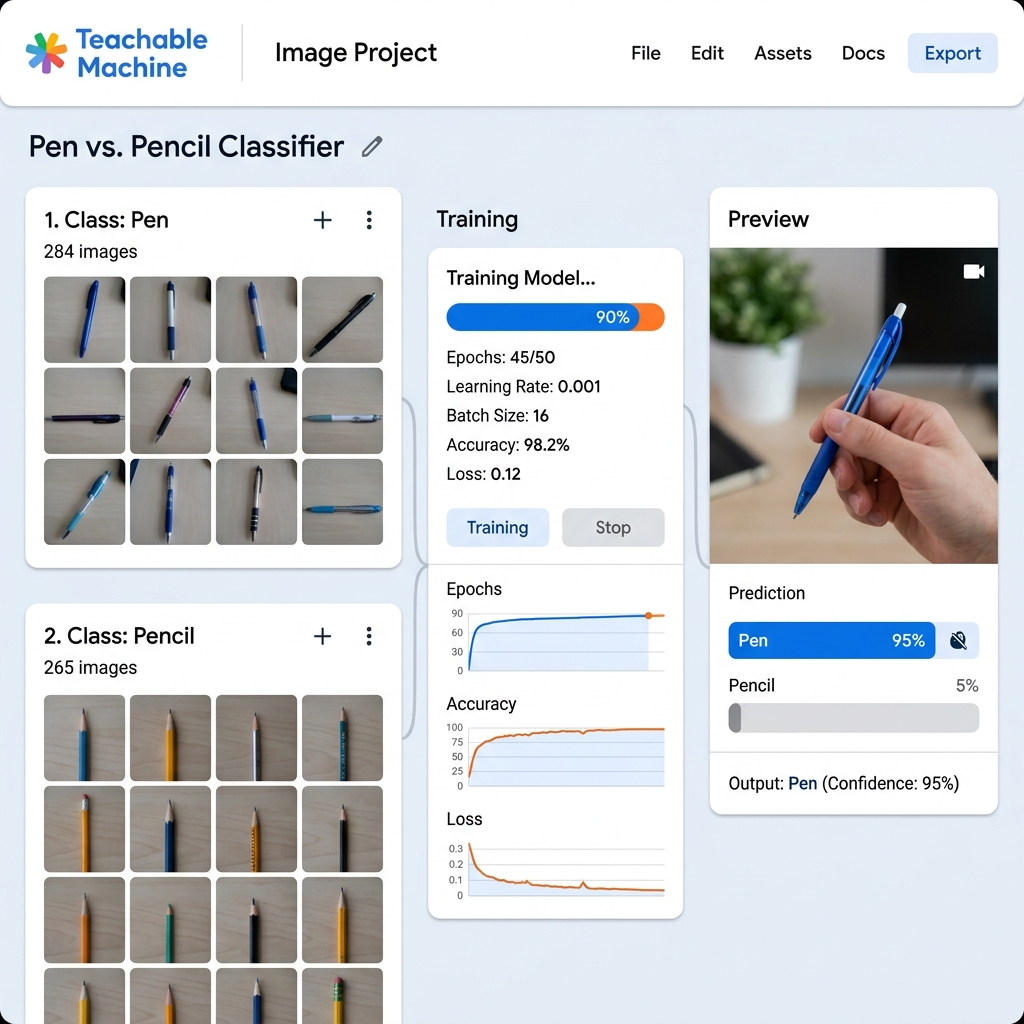
\includegraphics[width=0.82\linewidth]{images/teachable_machine_ui.jpg}
\caption[गूगल टीचेबल मशीन इंटरफ़ेस]{गूगल टीचेबल मशीन (Google Teachable Machine) का इंटरफ़ेस - जहाँ वेबकैम data द्वारा model को प्रशिक्षित किया जा रहा है।}
\label{fig:teachable-machine-ui}
\end{figure}

\section{AI के प्रकार (एक झलक)}
\begin{itemize}[leftmargin=1.4em]
  \item \eterm{Narrow AI} - केवल एक कार्य में निपुण (जैसे चेहरा पहचानना)।
        आज की लगभग सारी AI इसी प्रकार की है।
  \item \eterm{General AI} - मनुष्य जैसी सर्व-कार्य बुद्धि। यह अभी
        केवल अनुसन्धान (research) का विषय है।
\end{itemize}

\section{जनरेटिव AI एवं भाषा model (Generative AI \& LLMs)}

पिछले कुछ वर्षों में AI का एक नया रूप बहुत चर्चित हुआ है - \term{जनरेटिव
AI}{Generative AI}। यह केवल पहचानती ही नहीं, बल्कि \emph{नई सामग्री} (text, चित्र,
कोड, संगीत) स्वयं \emph{रचती} (generate) भी है। ChatGPT, Gemini एवं Claude जैसे
उपकरण इसी श्रेणी में आते हैं।

इनके मूल में \eterm{Large Language Model (LLM)} होते हैं - ऐसे
तंत्रिका जाल (neural networks) जिन्हें इंटरनेट के विशाल पाठ (text) पर प्रशिक्षित
किया जाता है। मूल रूप से ये \emph{“अगला शब्द क्या होगा”} का बार-बार पूर्वानुमान
करते हैं, और इसी से पूरे वाक्य एवं अनुच्छेद बन जाते हैं। एक सरल तंत्रिका जाल की
संरचना चित्र~\ref{fig:neural-net} में दिखाई गई है।

\begin{figure}[h]
\centering
\begin{tikzpicture}[font=\sffamily\footnotesize, >=Stealth,
    neuron/.style={circle, draw=aiblue, thick, minimum size=7mm, inner sep=0pt},
    ninp/.style={neuron, fill=ailite},
    nhid/.style={neuron, fill=aigreenL},
    nout/.style={neuron, fill=aiamberL}]
  \foreach \i in {1,2,3} \node[ninp]  (I\i) at (0, {2-\i}) {};
  \foreach \i in {1,2,3,4} \node[nhid] (H\i) at (2.2, {2.5-\i}) {};
  \foreach \i in {1,2} \node[nout] (O\i) at (4.4, {1-\i}) {};
  \foreach \i in {1,2,3} \foreach \j in {1,2,3,4} \draw[aigrey!50] (I\i) -- (H\j);
  \foreach \j in {1,2,3,4} \foreach \k in {1,2} \draw[aigrey!50] (H\j) -- (O\k);
  \node[aiblue, align=center]  at (0,1.4)   {\bfseries इनपुट\\\scriptsize Input};
  \node[aigreen, align=center] at (2.2,1.9) {\bfseries छिपी परतें\\\scriptsize Hidden};
  \node[aiamber, align=center] at (4.4,1.4) {\bfseries आउटपुट\\\scriptsize Output};
\end{tikzpicture}
\caption{एक सरल तंत्रिका जाल (neural network): इनपुट से छिपी परतों होते हुए आउटपुट तक।}
\label{fig:neural-net}
\end{figure}

\begin{jante}
ChatGPT का “GPT” का अर्थ है \emph{Generative Pre-trained Transformer}।
“Transformer” एक विशेष तंत्रिका-जाल रचना (architecture) है, जिसे सन् 2017 में
प्रस्तुत किया गया और जिसने आधुनिक भाषा मॉडलों की नींव रखी।
\end{jante}

\noindent\textbf{विज्ञान में उपयोग:} जनरेटिव AI शोध-पत्रों का सार बनाने, कोड लिखने में
सहायता, परिकल्पना (hypothesis) सुझाने, यहाँ तक कि नई औषधि-अणुओं एवं प्रोटीन-संरचनाओं
की रचना में भी सहायक है।

\begin{sochiye}
LLM कभी-कभी आत्मविश्वास से \emph{ग़लत} उत्तर भी दे देते हैं - इसे
\term{मतिभ्रम}{Hallucination} कहते हैं। इसलिए AI के उत्तर को किसी विश्वसनीय स्रोत से
सत्यापित करना क्यों आवश्यक है? कक्षा में चर्चा कीजिए।
\end{sochiye}

% ---------------- परियोजना ----------------
\begin{pariyojana}[मेरे आस-पास AI]
\textbf{उद्देश्य:} दैनिक जीवन एवं विज्ञान में AI की उपस्थिति पहचानना।\\[4pt]
\textbf{कार्य (समूह में, 3-4 विद्यार्थी):}
\begin{enumerate}[leftmargin=1.6em]
  \item एक सप्ताह तक ऐसे 10 स्थानों/उपकरणों की सूची बनाएँ जहाँ AI का उपयोग होता है
        (जैसे - मोबाइल कैमरा, YouTube सुझाव, मौसम ऐप, voice assistant)।
  \item प्रत्येक के सामने लिखें कि वह कौन-सा कार्य करती है - \emph{Perception,
        Learning, Reasoning या Decision}।
  \item इनमें से कौन-से उदाहरण किसी विज्ञान-विषय (Physics/Chemistry/Biology) से
        जुड़े हैं, चिह्नित करें।
  \item निष्कर्ष को एक पोस्टर या 5-स्लाइड प्रस्तुति (presentation) के रूप में
        कक्षा में दिखाएँ।
\end{enumerate}
\textbf{मूल्यांकन (assessment):} विविधता, वर्गीकरण की शुद्धता एवं प्रस्तुति की
स्पष्टता के आधार पर।
\end{pariyojana}

% ---------------- सारांश ----------------
\begin{bharatai}
भारत सरकार का \textbf{IndiaAI Mission} (2024) तथा \textbf{BHASHINI} परियोजना भारतीय
भाषाओं हेतु AI विकसित कर रही है - ताकि करोड़ों लोग अपनी ही भाषा में तकनीक का लाभ ले सकें।
\end{bharatai}

\section*{सारांश (Summary)}
\addcontentsline{toc}{section}{सारांश}
\begin{itemize}[leftmargin=1.4em]
  \item AI मशीनों को मानव-जैसे बौद्धिक कार्य करने योग्य बनाती है।
  \item Machine Learning, AI का वह भाग है जिसमें मशीन data से नियम स्वयं सीखती है।
  \item विशाल data के विश्लेषण में AI आधुनिक विज्ञान का शक्तिशाली उपकरण है।
  \item अंतिम वैज्ञानिक निर्णय सदैव मनुष्य के पास रहता है।
\end{itemize}

% ---------------- अभ्यास ----------------
\section*{अभ्यास (Exercises)}
\addcontentsline{toc}{section}{अभ्यास}
\textbf{अ. रिक्त स्थान भरिए:}
\begin{enumerate}[leftmargin=1.6em]
  \item \rule{2.5cm}{0.4pt}, AI का वह भाग है जिसमें मशीन data से सीखती है।
  \item आज की अधिकांश AI \rule{2.5cm}{0.4pt} (Narrow/General) प्रकार की है।
\end{enumerate}
\textbf{ब. लघु उत्तरीय:}
\begin{enumerate}[leftmargin=1.6em]
  \item परम्परागत प्रोग्रामिंग और Machine Learning में दो अंतर लिखिए।
  \item विज्ञान में AI उपयोगी होने के तीन कारण बताइए।
\end{enumerate}
\textbf{स. क्रियात्मक:}
\begin{enumerate}[leftmargin=1.6em]
  \item ऊपर की Teachable Machine गतिविधि दोहराएँ, परन्तु तीन class लेकर। accuracy
        पर क्या प्रभाव पड़ा?
\end{enumerate}

\begin{mcq}
  \item Machine Learning, निम्न में से किसका एक भाग है?
    \begin{choices}
      \item कृत्रिम बुद्धिमत्ता (AI) \item हार्डवेयर
      \item ऑपरेटिंग सिस्टम \item मॉनिटर
    \end{choices}
  \item “GPT” में अक्षर “T” किसका संक्षेप है?
    \begin{choices}
      \item Translator \item Transformer \item Transistor \item Transfer
    \end{choices}
  \item आज की अधिकांश AI किस प्रकार की है?
    \begin{choices}
      \item General AI \item Narrow AI
      \item अति-बुद्धि (Super AI) \item इनमें से कोई नहीं
    \end{choices}
  \item निम्न में से कौन-सा बुद्धिमत्ता का “Perception” कार्य है?
    \begin{choices}
      \item निष्कर्ष निकालना \item विकल्प चुनना
      \item चित्र/ध्वनि से जानकारी लेना \item नियम लागू करना
    \end{choices}
\end{mcq}

\begin{mukhyashabd}
\textbf{AI}, \textbf{Machine Learning (ML)}, \textbf{Deep Learning},
\textbf{Narrow AI}, \textbf{General AI},
\textbf{प्रत्यक्षण/अधिगम/तर्क/निर्णय}, \textbf{जनरेटिव AI (Generative AI)},
\textbf{वृहत् भाषा model (LLM)}, \textbf{Transformer}, \textbf{मतिभ्रम (Hallucination)}।
\end{mukhyashabd}
\selfcheckqr{https://kkreboot.github.io/ai-in-science-hindi/quiz/ch1.html}

\chapter{भौतिकी में कृत्रिम बुद्धिमत्ता}
\label{ch:physics}

\lakshyaheading
\begin{itemize}[leftmargin=1.4em]
  \item यह समझना कि भौतिकी मूलतः एक \emph{डेटा-विज्ञान (data science)} है।
  \item मापन (measurement), त्रुटि (error) एवं data के बीच सम्बन्ध।
  \item वक्र-संयोजन (curve fitting) एवं \term{समाश्रयण}{regression} द्वारा data से
        नियम (law) खोजना - जो भौतिकी में ML का हृदय है।
  \item कण भौतिकी (particle physics) एवं खगोल विज्ञान में पैटर्न-पहचान।
  \item मोबाइल सेंसर एवं Python की सहायता से वास्तविक data पर AI का प्रयोग।
\end{itemize}

\section{भौतिकी एक डेटा-विज्ञान है}

प्रत्येक भौतिक प्रयोग में हम कोई न कोई राशि मापते हैं - समय, दूरी, ताप, वोल्टता या
बल। ये सभी मान मिलकर \eterm{data} बनाते हैं। भौतिकी का मूल कार्य इन्हीं मानों में
छिपे \eterm{pattern} खोजकर एक \term{नियम}{law} तक पहुँचना है।

उदाहरण के लिए, गैलीलियो ने झुके हुए तल (inclined plane) पर लुढ़कती गेंद के समय एवं
दूरी के अनेक मान लिए, और उनमें यह pattern पहचाना कि $s \propto t^2$। यह ठीक वही कार्य है
जो आज एक Machine Learning model करता है - \emph{data से नियम सीखना}। अंतर केवल इतना है कि
गैलीलियो ने यह स्वयं किया, जबकि अब विशाल data पर यह कार्य मशीन तेज़ी से कर देती है।

\begin{jante}
सन् 2017 में खगोलविदों ने Google की एक \emph{neural network} की सहायता से NASA की
Kepler दूरबीन के पुराने data में दो नए ग्रह (\emph{exoplanets} - Kepler-90i तथा
Kepler-80g) खोजे, जिन्हें मनुष्य पहले चूक गए थे। मशीन ने वही प्रकाश-वक्र (light curve)
देखे, पर बहुत महीन pattern पकड़ लिया।
\end{jante}

\section{मापन, त्रुटि एवं data}

कोई भी मापन पूर्णतः सटीक नहीं होता - हर माप में कुछ \term{त्रुटि}{error} रहती है।
इसीलिए भौतिकी में एक ही राशि को कई बार मापा जाता है। इन मानों का \emph{माध्य (mean)}
सत्य के निकट होता है और उनका फैलाव (spread) त्रुटि का संकेत देता है।

\begin{itemize}[leftmargin=1.4em]
  \item \term{क्रमबद्ध त्रुटि}{Systematic error} - हर बार एक ही दिशा में (जैसे ग़लत
        अंशांकित स्केल)।
  \item \term{यादृच्छिक त्रुटि}{Random error} - हर बार बदलती हुई (जैसे प्रतिक्रिया-समय)।
\end{itemize}

AI के लिए यह बहुत महत्वपूर्ण है: यदि data में बहुत अधिक यादृच्छिक त्रुटि है (अर्थात्
data ``शोरयुक्त'' / \emph{noisy} है), तो model का पूर्वानुमान भी अनिश्चित होगा। इसीलिए
कहा जाता है - \emph{``अच्छा data ही अच्छी भौतिकी एवं अच्छी AI की नींव है।''}

\begin{sochiye}
यदि आप किसी लोलक (pendulum) का दोलन-काल केवल एक बार मापें बनाम 20 दोलनों का समय
मापकर उसे 20 से भाग दें - तो किसमें त्रुटि कम होगी और क्यों? यही विचार ML में ``अधिक
data से बेहतर परिणाम'' के सिद्धांत से कैसे जुड़ता है?
\end{sochiye}

\section{data से नियम: समाश्रयण (Regression)}

मान लीजिए आपके पास किसी प्रयोग के कुछ बिंदु (data points) हैं और आप उनके बीच से
सर्वोत्तम रेखा खींचना चाहते हैं। इस रेखा को खोजने की विधि को \term{रैखिक समाश्रयण}{Linear
Regression} कहते हैं। यह Machine Learning का सबसे सरल एवं सबसे महत्वपूर्ण model है।

रेखा का समीकरण होता है:
\[
  y = m x + c
\]
जहाँ $m$ ढलान (slope) तथा $c$ अंतःखंड (intercept) है। ML का कार्य ऐसे $m$ एवं $c$
खोजना है जिससे रेखा से बिंदुओं की लम्बवत् दूरियों के वर्गों का योग (कुल त्रुटि)
न्यूनतम हो। इसी ``वर्गों के योग को न्यूनतम करने'' के विचार को \term{अल्पतम वर्ग
विधि}{Least Squares Method} कहते हैं।

\begin{table}[h]
\centering
\begin{tabular}{@{}p{5cm} p{8cm}@{}}
\toprule
\rowcolor{cvBlue}\hdc{भौतिकी का प्रयोग} & \hdc{समाश्रयण किस नियम को ``सीखता'' है} \\
\midrule
स्प्रिंग पर बल बनाम विस्तार & हुक का नियम (Hooke's law), $F = kx$ \\
ओम का परिपथ (V बनाम I)      & ओम का नियम, $V = IR$ \\
गर्म वस्तु का ताप बनाम समय  & शीतलन (cooling) की प्रवृत्ति \\
\bottomrule
\end{tabular}
\caption{रैखिक समाश्रयण से भौतिकी के नियमों की पहचान}
\end{table}

ध्यान दें - model ``नियम'' को पहले से नहीं जानता; वह केवल data देखकर सर्वोत्तम $m$ एवं
$c$ निकालता है। यही ``data से सीखना'' का सार है। चित्र~\ref{fig:regression} में बिखरे
हुए डेटा-बिंदु एवं उनसे होकर गुज़रती सर्वोत्तम रेखा दिखाई गई है।

\begin{figure}[h]
\centering
\begin{tikzpicture}
\begin{axis}[
    width=10cm, height=6.2cm,
    font=\sffamily\small,
    xlabel={विस्तार $x$ (cm)}, ylabel={बल $F$ (N)},
    xmin=0, xmax=12, ymin=0, ymax=6,
    grid=both, grid style={aigrey!20},
    axis lines=left,
    legend pos=north west, legend cell align=left,
]
% डेटा-बिंदु (scatter)
\addplot[only marks, mark=*, aiblue, mark size=2.4pt]
  coordinates {(2,1.0) (4,2.1) (6,2.9) (8,4.2) (10,5.0)};
\addlegendentry{data}
% सर्वोत्तम रेखा (best-fit), लगभग F = 0.505 x
\addplot[thick, red, domain=0:11] {0.505*x + 0.01};
\addlegendentry{सर्वोत्तम रेखा (best-fit)}
\end{axis}
\end{tikzpicture}
\caption{रैखिक समाश्रयण (linear regression): बिखरे डेटा-बिंदुओं से होकर least-squares
द्वारा खींची गई सर्वोत्तम रेखा।}
\label{fig:regression}
\end{figure}

\begin{gatividhi}[हाथ से ``regression'' - सर्वोत्तम रेखा]
\textbf{लक्ष्य:} बिना कंप्यूटर के यह अनुभव करना कि model सर्वोत्तम रेखा कैसे खोजता है।\\[4pt]
\textbf{सामग्री:} ग्राफ़ पेपर, पैमाना, पेंसिल।\\[4pt]
\textbf{चरण:}
\begin{enumerate}[leftmargin=1.6em]
  \item किसी स्प्रिंग पर अलग-अलग भार लटकाकर विस्तार (extension) मापें - कम से कम 6 मान।
  \item बल ($F$) बनाम विस्तार ($x$) के बिंदु ग्राफ़ पर अंकित करें।
  \item आँख से ऐसी सीधी रेखा खींचें जो अधिकतम बिंदुओं के निकट हो (best-fit line)।
  \item रेखा की ढलान ($m$) निकालें - यही स्प्रिंग नियतांक (spring constant) $k$ है।
\end{enumerate}
\textbf{अवलोकन:} आपने जो किया, कंप्यूटर वही ``least squares'' से अधिक सटीकता से करता है।
\end{gatividhi}

\section{भौतिकी data पर Python (एक झलक)}

ऊपर की रेखा कंप्यूटर से खींचना बहुत सरल है। नीचे \emph{Google Colab} में चलने वाला एक
छोटा सा Python कोड है जो data पर सर्वोत्तम रेखा निकाल देता है। (यहाँ इसे समझना पर्याप्त
है; चलाना अध्याय~5 में सीखेंगे।)

\begin{lstlisting}
import numpy as np

# experiment data: force F (newton) vs extension x (metre)
x = np.array([0.02, 0.04, 0.06, 0.08, 0.10])   # extension
F = np.array([1.0, 2.1, 2.9, 4.2, 5.0])        # force

# best-fit line F = m*x + c   (degree 1 = straight line)
m, c = np.polyfit(x, F, 1)
print("spring constant k =", round(m, 2), "N/m")
\end{lstlisting}
\colabnb{https://colab.research.google.com/github/kkreboot/ai-in-science-hindi/blob/main/notebooks/ch2-spring.ipynb}

\noindent यहाँ \texttt{np.polyfit} ही least-squares regression कर रहा है - मात्र एक
पंक्ति में वही कार्य जो आपने गतिविधि में हाथ से किया था।

\section{पैटर्न-पहचान: कण भौतिकी एवं खगोल}

कुछ भौतिक प्रयोगों में data इतना विशाल होता है कि मनुष्य उसे देख ही नहीं सकता।

\subsection{कण भौतिकी (Particle Physics)}
\emph{CERN} के \eterm{Large Hadron Collider (LHC)} में प्रति सेकंड
लगभग एक अरब ($\approx 1$ billion) कण-टकराव (collisions) होते हैं। इनमें से अधिकांश साधारण हैं; केवल कुछ दुर्लभ
घटनाएँ (rare events) महत्वपूर्ण होती हैं। AI इन्हें छाँटकर वैज्ञानिकों तक पहुँचाती है।
सन् 2012 में \emph{Higgs boson} की खोज में भी ऐसी ही पैटर्न-पहचान तकनीकों का योगदान था।

\subsection{गुरुत्वीय तरंगें (Gravitational Waves)}
\emph{LIGO} वेधशाला अत्यंत क्षीण संकेतों को मापती है। दो ब्लैक होल के टकराने से उठी
तरंग का संकेत इतना कमज़ोर होता है कि वह ``शोर'' (noise) में दब जाता है। AI एवं
पैटर्न-मिलान (pattern matching) इन तरंगों को शोर से अलग पहचानने में सहायता करते हैं।

\subsection{खगोल विज्ञान (Astronomy)}
दूरबीनें (telescopes) प्रतिदिन लाखों आकाशीय पिंडों के चित्र भेजती हैं। AI इन विशाल
छवियों में आकाशगंगाओं (galaxies), तारों एवं दुर्लभ खगोलीय घटनाओं को स्वतः पहचान एवं
वर्गीकृत कर लेती है -- जिसे हाथ से करना असंभव होता। चित्र~\ref{fig:hubble} में हबल
दूरबीन द्वारा ली गई असंख्य दूरस्थ आकाशगंगाओं की एक झलक है।

\begin{figure}[h]
\centering
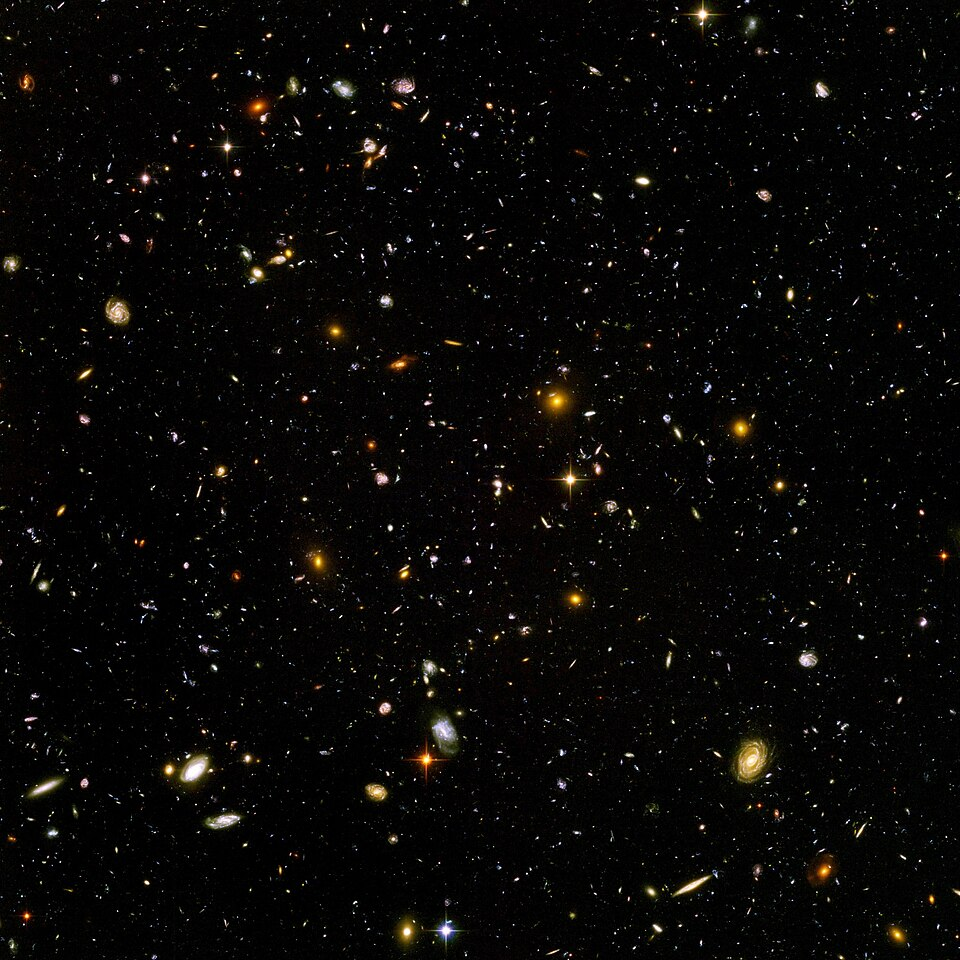
\includegraphics[width=0.62\linewidth]{images/hubble-udf.jpg}
\caption[हबल अल्ट्रा डीप फ़ील्ड -- हज़ारों आकाशगंगाएँ]{हबल अल्ट्रा डीप फ़ील्ड -- एक छोटे
से आकाश-क्षेत्र में हज़ारों आकाशगंगाएँ; AI ऐसी छवियों के विश्लेषण में सहायक
है।\imgsrc{NASA \& ESA, Wikimedia Commons (Public Domain)}}
\label{fig:hubble}
\end{figure}

\begin{jante}
\textbf{भारतीय योगदान: चंद्रयान-3 एवं ISRO (ISRO's Chandrayaan-3):}
भारतीय अंतरिक्ष अनुसंधान संगठन (ISRO) ने चंद्रयान-3 के 'प्रज्ञान रोवर' (Pragyan Rover) द्वारा भेजे गए चंद्र-सतह के चित्रों के विश्लेषण के लिए AI और कंप्यूटर विज़न (Computer Vision) का उपयोग किया। AI एल्गोरिदम रोवर के पथ में आने वाले गड्ढों (craters) और पत्थरों को स्वतः पहचानकर उसे सुरक्षित मार्ग पर बढ़ने में सहायता करते हैं। इसके अतिरिक्त, चंद्र-सतह के डिजिटल एलिवेशन model (Digital Elevation Models, DEM) बनाने में भी AI का महत्वपूर्ण योगदान रहा है।
\end{jante}

\begin{jante}
LHC प्रति सेकंड लगभग 1 \emph{petabyte} (दस लाख गीगाबाइट) data बनाता है - इसे संभालना
केवल AI एवं स्वचालित (automated) फ़िल्टर से ही सम्भव है।
\end{jante}

\section{पूर्वानुमान: गति एवं मौसम}

जब हम कुछ मापे गए मानों से अगली स्थिति का अनुमान लगाते हैं, उसे \term{पूर्वानुमान}{prediction}
कहते हैं।

\begin{itemize}[leftmargin=1.4em]
  \item \textbf{गति:} किसी प्रक्षेप्य (projectile) के कुछ बिंदु देकर उसका अगला पथ
        बताया जा सकता है - जैसे क्रिकेट में DRS की ``ball-tracking'' तकनीक।
  \item \textbf{मौसम:} तापमान, दाब एवं आर्द्रता के विशाल data से AI मौसम का
        पूर्वानुमान (weather forecasting) करती है। आधुनिक model अब पारंपरिक भौतिक
        समीकरणों के साथ-साथ ML का भी उपयोग करते हैं।
\end{itemize}

\begin{jante}
\textbf{भारतीय योगदान: मानसून का सटीक पूर्वानुमान (Monsoon Prediction by IISc):}
भारतीय विज्ञान संस्थान (IISc), बेंगलुरु और भारतीय मौसम विज्ञान विभाग (IMD) के शोधकर्ता भारत में मानसून की वर्षा के अधिक सटीक पूर्वानुमान के लिए कृत्रिम बुद्धिमत्ता (AI) और मशीन लर्निंग (ML) model का उपयोग कर रहे हैं। मानसून एक अत्यंत जटिल प्रणाली है जिसमें समुद्र के तापमान, हवा की दिशा और वायुमंडलीय दाब के बीच जटिल संबंध होते हैं। पारंपरिक सुपरकंप्यूटर भौतिक मॉडलों में जब Deep Learning को मिलाया जाता है, तो भारी वर्षा और अचानक आने वाली बाढ़ (flash floods) के पूर्वानुमान की सटीकता बहुत बढ़ जाती है।
\end{jante}

\begin{gatividhi}[मोबाइल सेंसर से वास्तविक भौतिक data]
\textbf{लक्ष्य:} वास्तविक भौतिक data एकत्र कर उसमें pattern देखना।\\[4pt]
\textbf{सामग्री:} स्मार्टफ़ोन, मुफ़्त ``Phyphox'' ऐप।\\[4pt]
\textbf{चरण:}
\begin{enumerate}[leftmargin=1.6em]
  \item ``Phyphox'' इंस्टॉल करें और ``Acceleration (without g)'' प्रयोग चुनें।
  \item फ़ोन को हाथ में लेकर धीरे ऊपर-नीचे घुमाएँ; data रिकॉर्ड करें।
  \item data को CSV रूप में निर्यात (export) करें और ग्राफ़ देखें।
  \item बताएँ - किस क्षण त्वरण (acceleration) अधिकतम था? ग्राफ़ का आकार आवर्ती
        (periodic) है या नहीं?
\end{enumerate}
\textbf{विस्तार:} यही CSV data Colab में खोलकर उस पर regression आज़माया जा सकता है।
\end{gatividhi}

\begin{figure}[h]
\centering
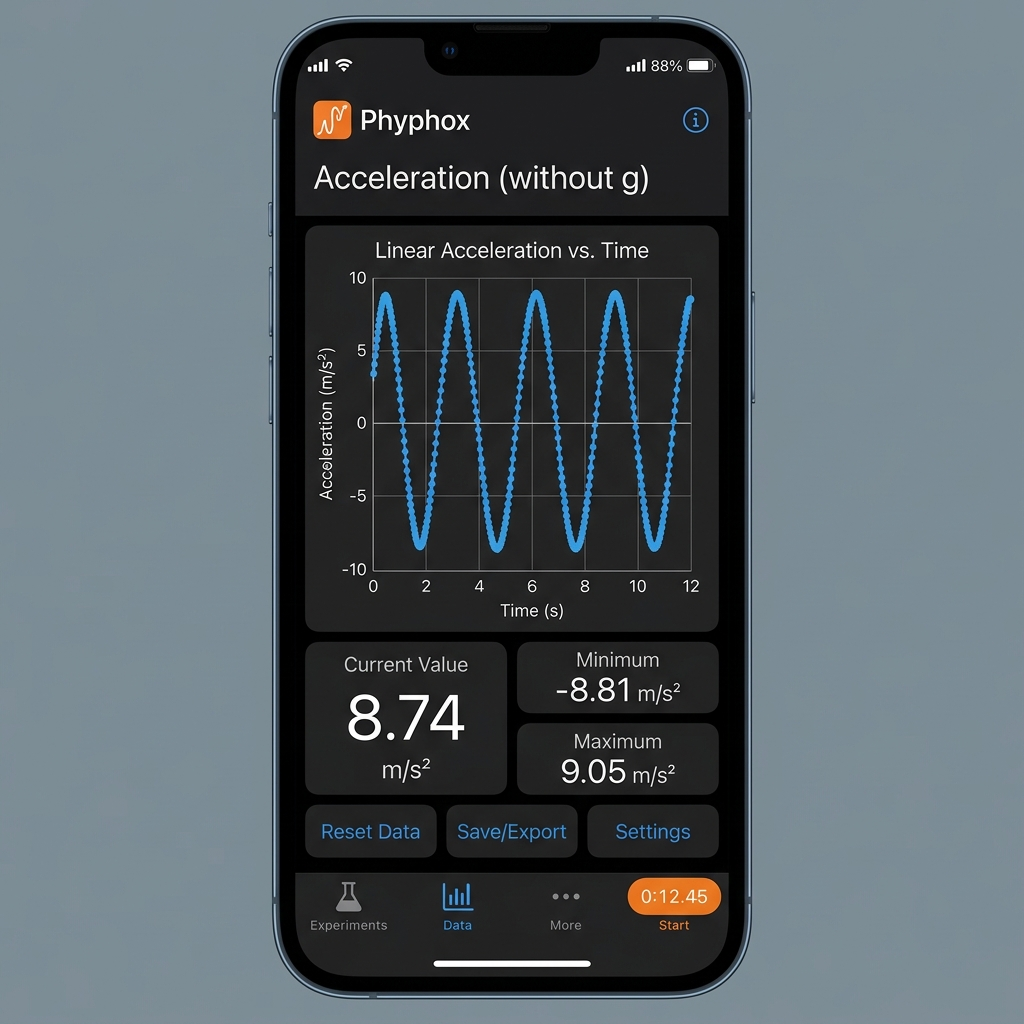
\includegraphics[width=0.48\linewidth]{images/phyphox_ui.jpg}
\caption[फिफॉक्स मोबाइल सेंसर इंटरफ़ेस]{स्मार्टफ़ोन में फिफॉक्स (Phyphox) ऐप का इंटरफ़ेस -- जहाँ त्वरण (acceleration) data को मापा और ग्राफ़ के रूप में देखा जा सकता है।}
\label{fig:phyphox-ui}
\end{figure}

% ---------------- परियोजना ----------------
\begin{pariyojana}[लोलक का दोलन-काल - मापन से पूर्वानुमान]
\textbf{उद्देश्य:} data से नियम सीखकर पूर्वानुमान करना, और उसे भौतिक सूत्र से जाँचना।\\[4pt]
\textbf{सामग्री:} धागा, छोटा भार (bob), पैमाना, स्टॉपवॉच (मोबाइल)।\\[4pt]
\textbf{कार्य (समूह में, 3–4 विद्यार्थी):}
\begin{enumerate}[leftmargin=1.6em]
  \item लोलक की लम्बाई $L$ को 6–7 भिन्न मानों पर लें (जैसे 20, 30, 40 \dots cm)।
  \item प्रत्येक लम्बाई पर 20 दोलनों का समय मापकर दोलन-काल $T$ निकालें।
  \item $T^2$ बनाम $L$ का ग्राफ़ बनाएँ - यह एक सीधी रेखा आनी चाहिए।
  \item रेखा से किसी \emph{नई} लम्बाई (जो आपने मापी नहीं) के लिए $T$ का पूर्वानुमान करें।
  \item अब वास्तव में उस लम्बाई पर मापकर देखें - पूर्वानुमान कितना सही था?
  \item परिणाम की तुलना सूत्र $T = 2\pi\sqrt{L/g}$ से करें तथा ग्राफ़ की ढलान से
        $g$ का मान निकालें।
\end{enumerate}
\textbf{मूल्यांकन:} data की शुद्धता, ग्राफ़, पूर्वानुमान की त्रुटि एवं $g$ के मान की
यथार्थता (accuracy) के आधार पर।
\end{pariyojana}

% ---------------- सारांश ----------------
\begin{bharatai}
पुणे का \textbf{GMRT} (विशाल रेडियो दूरबीन) एवं \textbf{AstroSat} जैसी भारतीय वेधशालाओं
से मिलने वाले विशाल खगोलीय data के विश्लेषण एवं पैटर्न-पहचान में AI का उपयोग बढ़ रहा है।
\end{bharatai}

\section*{सारांश (Summary)}
\addcontentsline{toc}{section}{सारांश}
\begin{itemize}[leftmargin=1.4em]
  \item भौतिकी मूलतः मापन एवं data पर आधारित विज्ञान है; नियम खोजना data में pattern
        खोजना ही है।
  \item हर मापन में त्रुटि रहती है; अधिक एवं स्वच्छ data बेहतर परिणाम देता है।
  \item रैखिक समाश्रयण (linear regression) data से नियम ``सीखने'' का सरलतम ML model है,
        जो least-squares द्वारा सर्वोत्तम रेखा खोजता है।
  \item कण भौतिकी, गुरुत्वीय तरंगों एवं खगोल में AI विशाल data से दुर्लभ pattern पहचानती है।
  \item मोबाइल सेंसर एवं Python जैसे मुफ़्त उपकरणों से विद्यार्थी स्वयं यह अनुभव कर सकते हैं।
\end{itemize}

% ---------------- अभ्यास ----------------
\section*{अभ्यास (Exercises)}
\addcontentsline{toc}{section}{अभ्यास}
\textbf{अ. रिक्त स्थान भरिए:}
\begin{enumerate}[leftmargin=1.6em]
  \item data में से सर्वोत्तम रेखा खोजने की ML विधि को \rule{2.8cm}{0.4pt} कहते हैं।
  \item सर्वोत्तम रेखा वह है जिससे बिंदुओं की कुल \rule{2.8cm}{0.4pt} न्यूनतम हो।
  \item हर बार एक ही दिशा में होने वाली त्रुटि \rule{2.8cm}{0.4pt} त्रुटि कहलाती है।
\end{enumerate}

\textbf{ब. लघु उत्तरीय:}
\begin{enumerate}[leftmargin=1.6em]
  \item ``भौतिकी एक डेटा-विज्ञान है'' - इस कथन को गैलीलियो के उदाहरण से समझाइए।
  \item रैखिक समाश्रयण किसी भौतिक नियम को कैसे ``सीखता'' है? एक उदाहरण दीजिए।
  \item कण भौतिकी (LHC) में AI क्यों आवश्यक है? संक्षेप में लिखिए।
\end{enumerate}

\textbf{स. क्रियात्मक / दीर्घ उत्तरीय:}
\begin{enumerate}[leftmargin=1.6em]
  \item स्प्रिंग वाली गतिविधि कीजिए और बताइए कि ढलान से स्प्रिंग नियतांक $k$ कैसे
        प्राप्त होता है।
  \item दिए गए data - $x:(1,2,3,4)$ तथा $y:(2,4,6,8)$ - के लिए हाथ से $m$ एवं $c$
        ज्ञात कीजिए। यह कौन-सा भौतिक सम्बन्ध दर्शाता है?
  \item Phyphox से एकत्र अपने त्वरण-data का ग्राफ़ बनाकर उसमें दिखने वाले pattern का
        वर्णन कीजिए।
\end{enumerate}

\begin{mcq}
  \item सरल रेखा $y=mx+c$ में $m$ क्या दर्शाता है?
    \begin{choices}\item अंतःखंड \item ढलान \item त्रुटि \item औसत\end{choices}
  \item data से सर्वोत्तम रेखा निकालने की विधि कहलाती है:
    \begin{choices}\item वर्गीकरण \item समाश्रयण (regression)
      \item क्रमबद्धन \item एन्क्रिप्शन\end{choices}
  \item गुरुत्वीय तरंगों को मापने वाली वेधशाला है:
    \begin{choices}\item LIGO \item LHC \item NASA \item ISRO\end{choices}
  \item Higgs boson की खोज किस संस्था के प्रयोग से जुड़ी है?
    \begin{choices}\item CERN \item NCBI \item PubChem \item WHO\end{choices}
\end{mcq}

\begin{mukhyashabd}
\textbf{data}, \textbf{pattern}, \textbf{नियम (law)}, \textbf{त्रुटि (error)} --
क्रमबद्ध एवं यादृच्छिक, \textbf{रैखिक समाश्रयण (Linear Regression)},
\textbf{अल्पतम वर्ग विधि (Least Squares)}, \textbf{पूर्वानुमान (prediction)},
\textbf{LHC}, \textbf{LIGO}।
\end{mukhyashabd}
\selfcheckqr{https://kkreboot.github.io/ai-in-science-hindi/quiz/ch2.html}

\chapter{रसायन विज्ञान में कृत्रिम बुद्धिमत्ता}
\label{ch:chemistry}

\lakshyaheading
\begin{itemize}[leftmargin=1.4em]
  \item अणु (molecule) एवं अभिक्रिया (reaction) को \emph{data} के रूप में देखना।
  \item आवर्त सारणी (periodic table) के गुणों में pattern एवं प्रवृत्ति (trend) पहचानना।
  \item \term{वर्गीकरण}{classification} एवं \term{पूर्वानुमान}{prediction} द्वारा
        पदार्थों के गुण आँकना।
  \item दवा-खोज (drug discovery) एवं नई सामग्री (materials) में AI की भूमिका।
  \item मुफ़्त उपकरणों से अणु एवं data पर स्वयं प्रयोग करना।
\end{itemize}

\section{अणु भी एक data हैं}

प्रत्येक अणु को उसके परमाणुओं (atoms) एवं उनके बीच के बंधों (bonds) की एक संरचना
(structure) के रूप में लिखा जा सकता है। यदि इस संरचना को संख्याओं में बदल दिया जाए, तो
कंप्यूटर लाखों अणुओं की आपस में तुलना कर सकता है और बता सकता है कि कौन-सा अणु किसी विशेष
\term{गुण}{property} वाला हो सकता है।

एक प्रचलित तरीका है \eterm{SMILES notation}, जिसमें अणु को एक छोटी
पंक्ति (string) के रूप में लिखते हैं। उदाहरण के लिए, जल (H\textsubscript{2}O) को \texttt{O},
तथा एथेनॉल को \texttt{CCO} लिखा जाता है। AI ऐसे संकेतों को पढ़कर अणु को ``समझ'' लेती है।
किसी अणु की त्रि-आयामी (3D) संरचना भी data ही है, जैसा चित्र~\ref{fig:caffeine} में
कैफ़ीन (caffeine) अणु के लिए दिखाया गया है।

\begin{figure}[h]
\centering
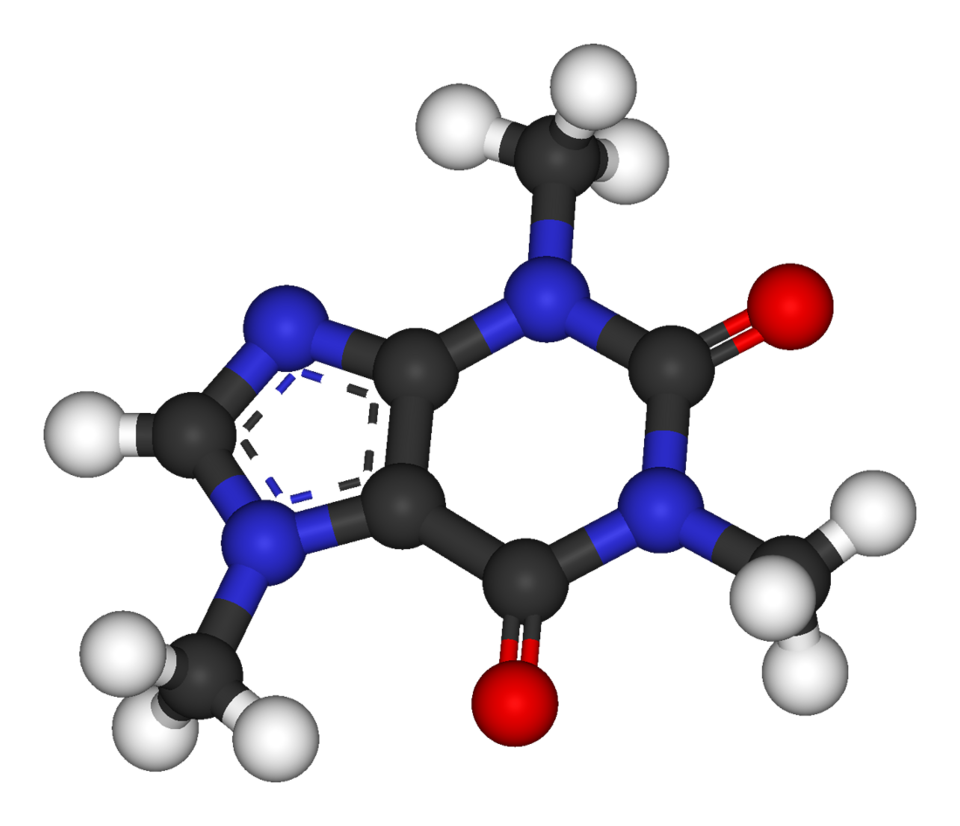
\includegraphics[width=0.45\linewidth]{images/caffeine.png}
\caption[कैफ़ीन अणु का त्रि-आयामी model]{कैफ़ीन अणु का त्रि-आयामी (ball-and-stick) model --
परमाणु एवं बंध ही वह ``data'' हैं जिन्हें AI पढ़ती है।\imgsrc{Wikimedia Commons (Public Domain)}}
\label{fig:caffeine}
\end{figure}

\begin{jante}
दुनिया में सैद्धांतिक रूप से सम्भव \emph{औषधि-सदृश} (drug-like) छोटे कार्बनिक अणुओं
की संख्या $10^{60}$ से भी अधिक आँकी गई है - इतने अणुओं को मनुष्य कभी हाथ से नहीं जाँच सकता, पर
AI उन्हें छाँट (screen) सकती है।
\end{jante}

\section{pattern: आवर्त सारणी की भाषा}

रसायन विज्ञान में पैटर्न-पहचान का सबसे सुंदर उदाहरण स्वयं \term{आवर्त सारणी}{Periodic
Table} है। मेंडेलीफ़ (Mendeleev) ने तत्वों के गुणों में प्रवृत्ति देखकर न केवल उन्हें
क्रम में रखा, बल्कि कुछ \emph{अनदेखे तत्वों} के गुणों का \emph{पूर्वानुमान} भी कर दिया -
जो बाद में सही निकले। यही ``data से पूर्वानुमान'' का विचार आज ML करता है।

\begin{table}[h]
\centering
\begin{tabular}{@{}p{4.6cm} p{8.4cm}@{}}
\toprule
\rowcolor{cvBlue}\hdc{प्रवृत्ति (trend)} & \hdc{आवर्त में (बाएँ से दाएँ) क्या होता है} \\
\midrule
परमाणु त्रिज्या (atomic radius) & घटती है \\
आयनन ऊर्जा (ionisation energy)  & बढ़ती है \\
विद्युत्‌ऋणात्मकता (electronegativity) & बढ़ती है \\
\bottomrule
\end{tabular}
\caption{आवर्त सारणी में दिखने वाली नियमित प्रवृत्तियाँ - pattern का आधार}
\end{table}

\begin{sochiye}
मेंडेलीफ़ ने ``eka-silicon'' (बाद में Germanium) के गुणों का पूर्वानुमान बिना उस तत्व
को देखे किया। उन्होंने किस आधार पर यह किया, और यह आज के Machine Learning के
``prediction'' से किस प्रकार मिलता-जुलता है? चर्चा कीजिए।
\end{sochiye}

\section{वर्गीकरण एवं पूर्वानुमान (Classification \& Prediction)}

रसायन में AI के दो सबसे सामान्य कार्य हैं:
\begin{itemize}[leftmargin=1.4em]
  \item \textbf{वर्गीकरण (classification):} किसी पदार्थ को श्रेणियों में बाँटना -
        जैसे ``अम्ल या क्षार'', ``विलेय या अविलेय'', ``विषैला या सुरक्षित''।
  \item \textbf{पूर्वानुमान (regression/prediction):} किसी सतत गुण का मान आँकना -
        जैसे क्वथनांक (boiling point), घुलनशीलता (solubility) या अभिक्रिया की दर
        (rate)।
\end{itemize}

इन दोनों के लिए मशीन को पहले बहुत-से ज्ञात उदाहरण (training data) दिए जाते हैं - जैसे
हज़ारों अणु और उनके मापे गए क्वथनांक। मशीन इनसे सम्बन्ध सीखकर किसी \emph{नए} अणु का
क्वथनांक बता देती है।

\begin{gatividhi}[आवर्त सारणी में प्रवृत्ति का ``regression'']
\textbf{लक्ष्य:} data में रुझान पहचानकर एक अनदेखे मान का पूर्वानुमान करना।\\[4pt]
\textbf{सामग्री:} ग्राफ़ पेपर, आवर्त सारणी (डेटा-पुस्तिका)।\\[4pt]
\textbf{चरण:}
\begin{enumerate}[leftmargin=1.6em]
  \item आवर्त-2 के तत्वों (Li, Be, B, C, N, O, F) का परमाणु क्रमांक एवं परमाणु
        त्रिज्या एक तालिका में लिखें।
  \item परमाणु क्रमांक (x) बनाम त्रिज्या (y) का ग्राफ़ बनाएँ।
  \item बिना मान देखे, किसी एक तत्व को छिपाकर उसकी त्रिज्या का पूर्वानुमान करें।
  \item वास्तविक मान से तुलना करें - आपकी त्रुटि कितनी रही?
\end{enumerate}
\textbf{अवलोकन:} आपने वही किया जो एक ML ``regression'' model करता है - ज्ञात बिंदुओं से
अनदेखे मान का अनुमान।
\end{gatividhi}

\section{दवा-खोज में AI (Drug Discovery)}

एक नई दवा बनाने में सामान्यतः 10–15 वर्ष एवं हज़ारों करोड़ रुपये लग जाते हैं, क्योंकि
लाखों अणुओं में से सही अणु खोजना पड़ता है। AI इस प्रक्रिया को इस प्रकार तेज़ करती है:

\begin{enumerate}[leftmargin=1.6em]
  \item \term{आभासी छँटाई}{Virtual Screening} - कंप्यूटर पर ही लाखों अणुओं को
        जाँचकर सम्भावित दवाओं की छोटी सूची बनाना।
  \item \term{गुण-पूर्वानुमान}{Property Prediction} - विषाक्तता (toxicity) एवं
        घुलनशीलता पहले से आँकना, ताकि असफल अणु जल्दी हट जाएँ।
  \item \term{अणु-अभिकल्प}{Molecule Design} - वांछित गुण वाले नए अणु ``सुझाना''।
\end{enumerate}

\begin{figure}[h]
\centering
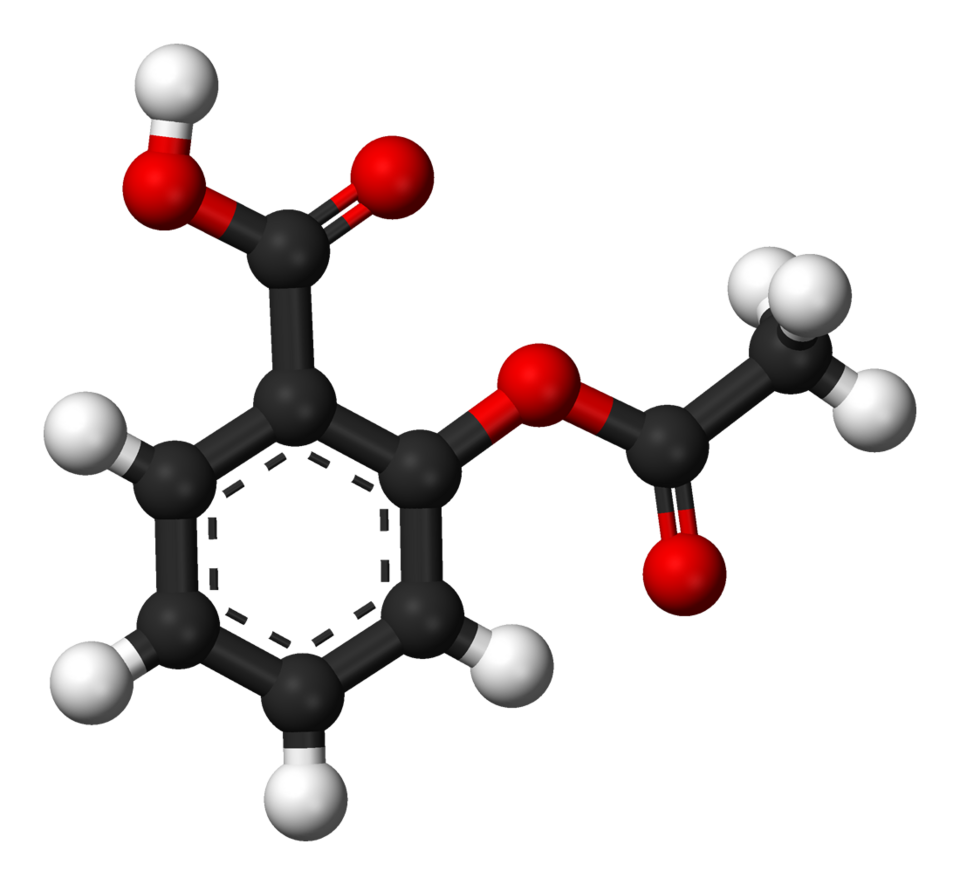
\includegraphics[width=0.45\linewidth]{images/aspirin.png}
\caption[एस्पिरिन अणु का 3D model]{एस्पिरिन (aspirin) अणु का 3D model -- AI ऐसे हज़ारों
दवा-अणुओं की संरचना एवं गुणों की तुलना कर सम्भावित औषधियाँ छाँटती है।\imgsrc{Wikimedia Commons (Public Domain)}}
\label{fig:aspirin}
\end{figure}

\begin{jante}
सन् 2020 में MIT के शोधकर्ताओं ने एक AI model से \emph{Halicin} नामक नया एंटीबायोटिक
खोजा। यह दवा परम्परागत एंटीबायोटिक से संरचना में बिल्कुल भिन्न थी, और कई दवा-प्रतिरोधी
(drug-resistant) बैक्टीरिया पर भी कारगर निकली।
\end{jante}

\section{नई सामग्री एवं हरित रसायन (Materials \& Green Chemistry)}

AI केवल दवाओं तक सीमित नहीं - इससे बेहतर \emph{बैटरी पदार्थ}, मज़बूत मिश्रधातु
(alloys), और कुशल \term{उत्प्रेरक}{catalysts} भी खोजे जा रहे हैं। उत्प्रेरक की सही खोज
से अभिक्रियाएँ कम ऊर्जा एवं कम अपशिष्ट (waste) के साथ होती हैं - जो ``हरित रसायन''
(green chemistry) का लक्ष्य है।

\section{रसायन data पर Python (एक झलक)}

नीचे का छोटा कोड दिखाता है कि किसी सरल data (ताप बनाम विलेयता) पर मशीन सर्वोत्तम वक्र
कैसे निकाल सकती है। (इसे चलाना अध्याय~5 में सीखेंगे; यहाँ विचार समझना पर्याप्त है।)

\begin{lstlisting}
import numpy as np

# solubility of a salt: temperature T (deg C), solubility S (g / 100 mL water)
T = np.array([10, 20, 30, 40, 50])
S = np.array([31, 34, 37, 40, 43])

# best-fit straight line S = a*T + b
a, b = np.polyfit(T, S, 1)
T_new = 35
print("predicted solubility at 35 C =", round(a*T_new + b, 1), "g/100mL")
\end{lstlisting}
\colabnb{https://colab.research.google.com/github/kkreboot/ai-in-science-hindi/blob/main/notebooks/ch3-solubility.ipynb}

\noindent यहाँ model किसी रासायनिक सूत्र को नहीं जानता - वह केवल data से प्रवृत्ति सीखकर
मध्यवर्ती ताप पर विलेयता का पूर्वानुमान कर देता है।

\begin{gatividhi}[बिना कोड - अणुओं का दृश्य अन्वेषण]
\textbf{लक्ष्य:} अणु को त्रि-आयामी (3D) संरचना के रूप में ``data'' की तरह देखना।\\[4pt]
\textbf{सामग्री:} इंटरनेट, ``MolView'' (molview.org) या PubChem वेबसाइट।\\[4pt]
\textbf{चरण:}
\begin{enumerate}[leftmargin=1.6em]
  \item MolView पर जल (\texttt{water}), एथेनॉल एवं ग्लूकोज़ खोजें।
  \item प्रत्येक अणु की 3D संरचना घुमाकर देखें; बंध-कोण (bond angle) देखें।
  \item SMILES संकेत (जैसे एथेनॉल = \texttt{CCO}) नोट करें - यही वह ``data'' है जिसे
        AI पढ़ती है।
\end{enumerate}
\end{gatividhi}

\begin{figure}[h]
\centering
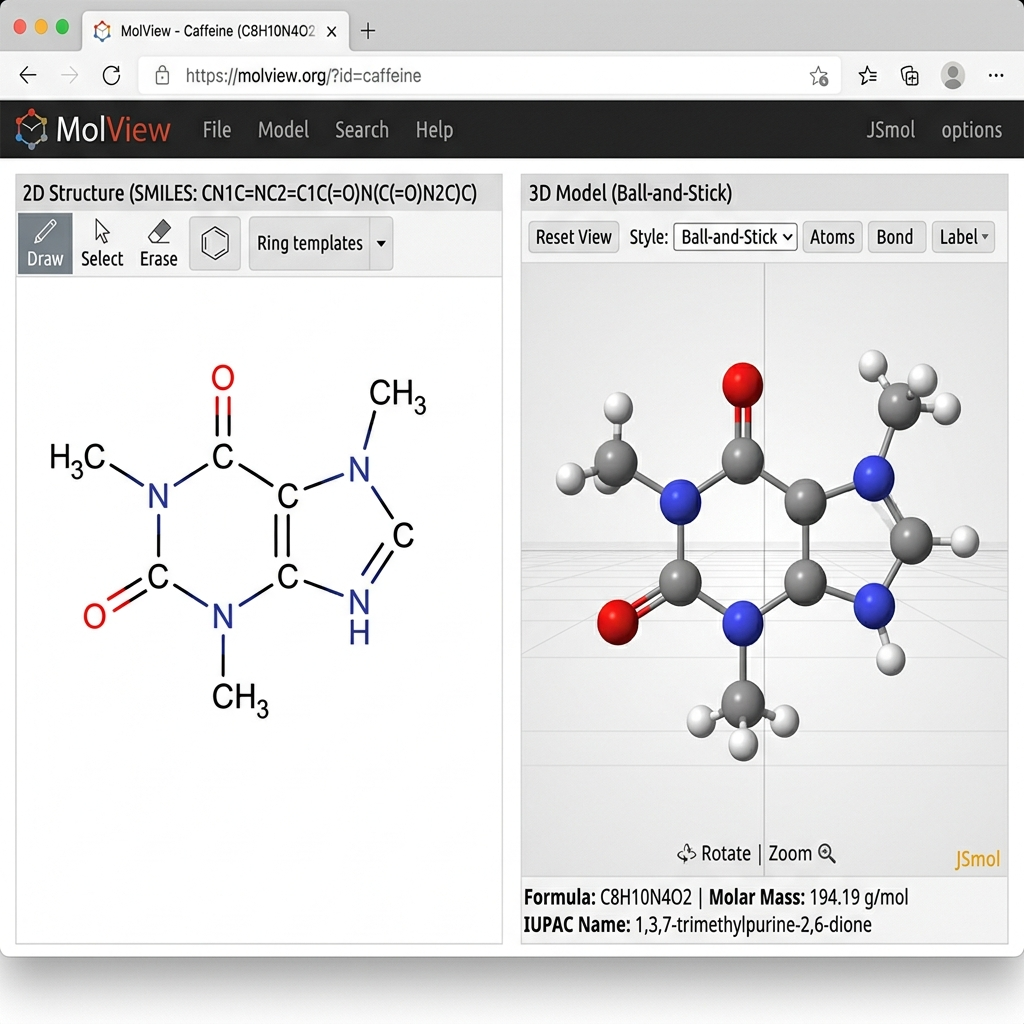
\includegraphics[width=0.72\linewidth]{images/molview_ui.jpg}
\caption[मॉलव्यू आणविक दृश्य अन्वेषण]{मॉलव्यू (MolView) वेबसाइट का इंटरफ़ेस -- जहाँ बाईं ओर 2D संरचना और दाईं ओर कैफीन (Caffeine) अणु का 3D model (Ball-and-Stick) दर्शाया गया है।}
\label{fig:molview-ui}
\end{figure}

% ---------------- परियोजना ----------------
\begin{pariyojana}[विलेयता का पूर्वानुमान - प्रयोग से सत्यापन]
\textbf{उद्देश्य:} वास्तविक प्रयोग का data एकत्र कर उससे पूर्वानुमान करना एवं उसे
प्रयोग से जाँचना।\\[4pt]
\textbf{सामग्री:} सामान्य नमक या चीनी, जल, बीकर, थर्मामीटर, तुला (balance)।\\[4pt]
\textbf{कार्य (समूह में, 3–4 विद्यार्थी):}
\begin{enumerate}[leftmargin=1.6em]
  \item विभिन्न तापमानों (जैसे 20, 30, 40, 50\,$^\circ$C) पर 100\,mL जल में अधिकतम
        घुलने वाले पदार्थ की मात्रा मापें।
  \item ताप बनाम विलेयता का ग्राफ़ बनाएँ तथा सर्वोत्तम रेखा/वक्र खींचें।
  \item ग्राफ़ से किसी \emph{नए} तापमान (जैसे 35\,$^\circ$C) पर विलेयता का पूर्वानुमान करें।
  \item अब वास्तव में उस ताप पर मापकर पूर्वानुमान की त्रुटि ज्ञात करें।
  \item चर्चा करें - data बिंदु बढ़ाने पर पूर्वानुमान बेहतर हुआ या नहीं?
\end{enumerate}
\textbf{मूल्यांकन:} मापन की शुद्धता, ग्राफ़, पूर्वानुमान-त्रुटि एवं निष्कर्ष की
स्पष्टता के आधार पर।
\end{pariyojana}

% ---------------- सारांश ----------------
\section*{सारांश (Summary)}
\addcontentsline{toc}{section}{सारांश}
\begin{itemize}[leftmargin=1.4em]
  \item अणु को संरचना/SMILES के रूप में संख्याओं में बदलकर AI लाखों अणुओं की तुलना
        कर सकती है।
  \item आवर्त सारणी की प्रवृत्तियाँ पैटर्न-पहचान एवं पूर्वानुमान का उत्कृष्ट उदाहरण हैं।
  \item रसायन में AI के दो प्रमुख कार्य हैं - वर्गीकरण (classification) एवं
        गुण-पूर्वानुमान (prediction)।
  \item दवा-खोज, नई सामग्री एवं हरित रसायन में AI समय एवं लागत बहुत घटा देती है।
  \item मुफ़्त उपकरण (MolView, PubChem) एवं सरल Python से विद्यार्थी स्वयं यह अनुभव कर
        सकते हैं।
\end{itemize}

% ---------------- अभ्यास ----------------
\section*{अभ्यास (Exercises)}
\addcontentsline{toc}{section}{अभ्यास}
\textbf{अ. रिक्त स्थान भरिए:}
\begin{enumerate}[leftmargin=1.6em]
  \item अणु को एक पंक्ति (string) के रूप में लिखने की विधि \rule{2.8cm}{0.4pt} कहलाती है।
  \item किसी पदार्थ को ``अम्ल या क्षार'' श्रेणियों में बाँटना AI का \rule{2.8cm}{0.4pt} कार्य है।
  \item दवा-खोज में लाखों अणुओं को कंप्यूटर पर जाँचने को \rule{2.8cm}{0.4pt} कहते हैं।
\end{enumerate}

\textbf{ब. लघु उत्तरीय:}
\begin{enumerate}[leftmargin=1.6em]
  \item मेंडेलीफ़ का अनदेखे तत्वों का पूर्वानुमान आधुनिक ML से किस प्रकार मिलता है?
  \item classification एवं prediction (regression) में अंतर एक-एक रासायनिक उदाहरण से बताइए।
  \item दवा-खोज में AI के कोई तीन उपयोग लिखिए।
\end{enumerate}

\textbf{स. क्रियात्मक / दीर्घ उत्तरीय:}
\begin{enumerate}[leftmargin=1.6em]
  \item आवर्त-2 के तत्वों की त्रिज्या वाली गतिविधि कीजिए तथा अपने पूर्वानुमान की त्रुटि
        लिखिए।
  \item MolView पर तीन अणुओं की 3D संरचना देखिए और उनके SMILES संकेत लिखिए।
  \item ``AI नई दवाओं की खोज को कैसे तेज़ करती है'' - इस पर एक संक्षिप्त निबंध लिखिए।
\end{enumerate}

\begin{mcq}
  \item अणु को एक छोटी पंक्ति (string) के रूप में लिखने का संकेतन है:
    \begin{choices}\item SMILES \item HTML \item JSON \item SQL\end{choices}
  \item आवर्त सारणी में अनदेखे तत्वों का पूर्वानुमान किसने किया?
    \begin{choices}\item डाल्टन \item मेंडेलीफ़ \item रदरफोर्ड \item बोर\end{choices}
  \item कंप्यूटर पर लाखों अणुओं को जाँचकर दवा छाँटना कहलाता है:
    \begin{choices}\item आभासी छँटाई (virtual screening) \item आसवन
      \item क्रिस्टलन \item अनुमापन\end{choices}
  \item AI से खोजा गया नया एंटीबायोटिक (2020) था:
    \begin{choices}\item पेनिसिलिन \item हैलिसिन (Halicin)
      \item एस्पिरिन \item इंसुलिन\end{choices}
\end{mcq}

\begin{mukhyashabd}
\textbf{स्माइल्स संकेतन (SMILES)}, \textbf{वर्गीकरण (classification)},
\textbf{पूर्वानुमान (prediction)}, \textbf{आभासी छँटाई (Virtual Screening)},
\textbf{गुण-पूर्वानुमान (Property Prediction)}, \textbf{अणु-अभिकल्प (Molecule Design)},
\textbf{उत्प्रेरक (catalyst)}।
\end{mukhyashabd}
\selfcheckqr{https://kkreboot.github.io/ai-in-science-hindi/quiz/ch3.html}

\chapter{जीव विज्ञान में कृत्रिम बुद्धिमत्ता}
\label{ch:biology}

\lakshyaheading
\begin{itemize}[leftmargin=1.4em]
  \item जीवन की जानकारी को \emph{डेटा} के रूप में समझना - विशेषकर DNA एवं प्रोटीन।
  \item प्रोटीन-संरचना (protein structure) के पूर्वानुमान में AI (AlphaFold)।
  \item चिकित्सा-चित्रों (medical images) में रोग-पहचान हेतु \term{चित्र-वर्गीकरण}{image
        classification}।
  \item प्रजाति-पहचान (species identification) एवं जैव-विविधता में AI।
  \item मुफ़्त उपकरणों एवं सरल Python से जैविक डेटा पर स्वयं प्रयोग।
\end{itemize}

\section{जीवन का डेटा: DNA}

हमारे शरीर की लगभग सम्पूर्ण जानकारी DNA में, केवल चार ``अक्षरों'' - A, T, G, C
(\term{क्षारक}{bases}) - के क्रम में लिखी होती है। मनुष्य के DNA में ऐसे लगभग
3 अरब (3 billion) अक्षर होते हैं। यह इतना विशाल \term{डेटा}{data} है कि इसका विश्लेषण
AI के बिना लगभग असम्भव है।

इन अक्षरों के क्रम (sequence) में ही यह छिपा होता है कि कौन-सा प्रोटीन बनेगा और कोशिका
कैसे कार्य करेगी। AI इन क्रमों में पैटर्न खोजकर बता सकती है कि कोई विशेष क्रम किसी रोग
से जुड़ा है या नहीं - इसी क्षेत्र को \term{जैव-सूचना विज्ञान}{Bioinformatics} कहते हैं।
DNA की द्विकुंडलिनी (double helix) संरचना चित्र~\ref{fig:dna} में दिखाई गई है।

\begin{figure}[h]
\centering
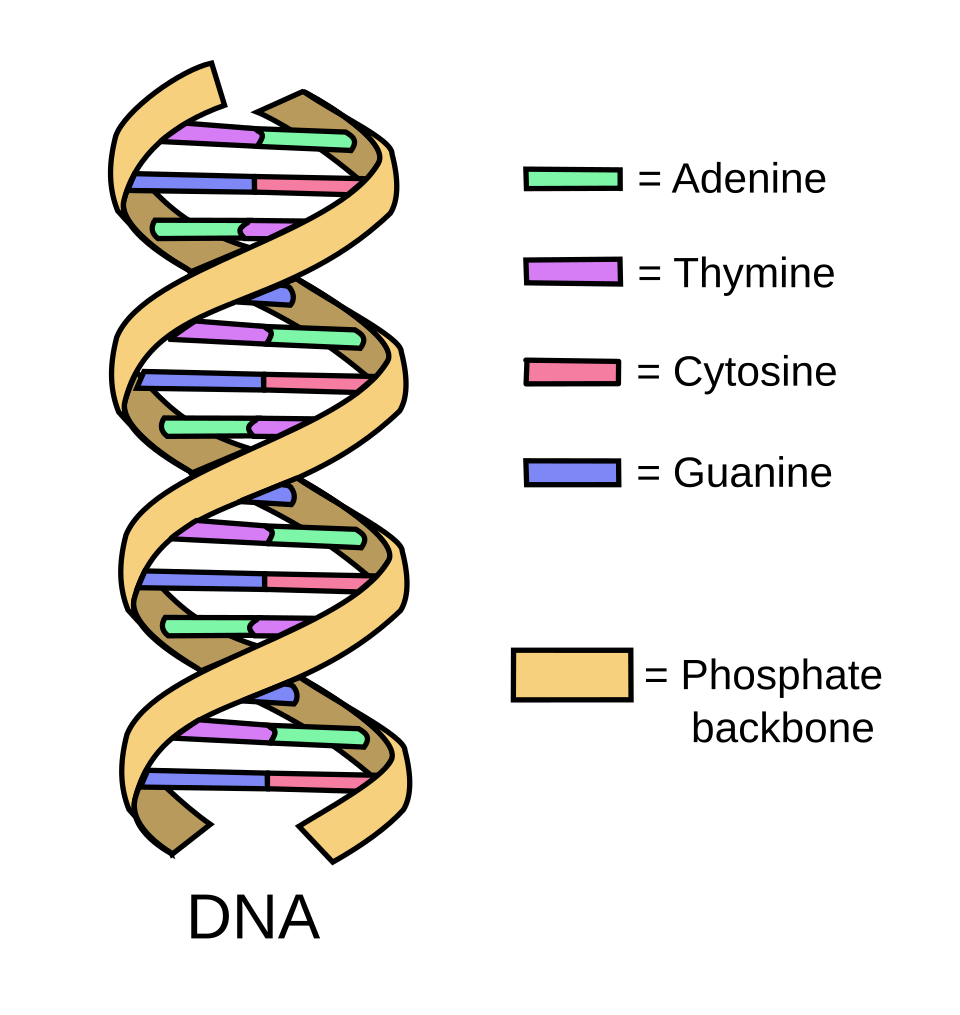
\includegraphics[height=5.2cm]{images/dna.png}
\caption[DNA की द्विकुंडलिनी (double helix)]{DNA की द्विकुंडलिनी (double helix) -- A, T,
G, C क्षारकों का क्रम ही जीवन का विशाल ``डेटा'' है, जिसे AI पढ़ती एवं विश्लेषित करती
है।\imgsrc{Forluvoft, Wikimedia Commons (Public Domain)}}
\label{fig:dna}
\end{figure}

\begin{jante}
मानव जीनोम (human genome) को पूरा पढ़ने वाली ``Human Genome Project'' परियोजना (2003)
में लगभग 13 वर्ष लगे थे। आज वही कार्य उन्नत मशीनों एवं AI की सहायता से कुछ ही घंटों में
सम्भव है।
\end{jante}

\section{प्रोटीन की संरचना: AlphaFold}

प्रोटीन (protein) अमीनो अम्लों (amino acids) की एक लम्बी शृंखला से बनते हैं, परन्तु उनका
कार्य उनकी \emph{त्रि-आयामी (3D) मुड़ी हुई संरचना} पर निर्भर करता है। किसी क्रम से उसकी
3D संरचना का पूर्वानुमान करना दशकों तक जीव विज्ञान की सबसे कठिन समस्याओं में से एक था,
जिसे \term{प्रोटीन-वलन समस्या}{Protein Folding Problem} कहते हैं।

सन् 2021 में DeepMind के \emph{AlphaFold} नामक AI ने इस समस्या को हल करने में ऐतिहासिक
सफलता पाई, और 2022 तक लगभग सभी ज्ञात प्रोटीनों (लगभग 20 करोड़) की 3D संरचना का सटीक
पूर्वानुमान कर दिया। यह AI की सहायता से विज्ञान की एक ऐतिहासिक उपलब्धि
मानी जाती है, क्योंकि इससे नई दवाओं एवं एंज़ाइमों (enzymes) की खोज बहुत तेज़ हो गई।
मूल विचार चित्र~\ref{fig:alphafold} में दर्शाया गया है: एक अमीनो-अम्ल क्रम (input) से
AI सीधे प्रोटीन की 3D संरचना (output) का पूर्वानुमान कर देती है।

\begin{figure}[h]
\centering
\begin{tikzpicture}[font=\sffamily\small, node distance=10mm,
    box/.style={draw=aiblue, thick, fill=ailite, rounded corners,
      minimum height=1.5cm, text width=3cm, align=center, inner sep=4pt},
    ai/.style={draw=aigreen, very thick, fill=aigreenL, rounded corners,
      minimum height=1.5cm, text width=2.6cm, align=center},
    arr/.style={-{Stealth[length=3mm]}, very thick, aigrey}]
  \node[box] (seq) {\footnotesize अमीनो-अम्ल क्रम\\\ttfamily\scriptsize M-K-T-A-Y-\dots};
  \node[ai, right=of seq] (af) {\bfseries AI\\\footnotesize (AlphaFold)};
  \node[box, right=of af] (str) {\footnotesize 3D प्रोटीन संरचना\\\footnotesize (folded structure)};
  \draw[arr] (seq) -- (af) node[midway, above, aigrey, font=\scriptsize] {input};
  \draw[arr] (af) -- (str) node[midway, above, aigrey, font=\scriptsize] {output};
\end{tikzpicture}
\caption{AlphaFold का मूल विचार: क्रम (sequence) से सीधे प्रोटीन की 3D संरचना का
पूर्वानुमान।}
\label{fig:alphafold}
\end{figure}

\begin{sochiye}
एक ही अमीनो-अम्ल क्रम सदैव एक ही आकार में मुड़ता है। इसका अर्थ है कि ``क्रम'' में ही
``आकार'' की जानकारी छिपी है। यह विचार Machine Learning के ``input से output का
पूर्वानुमान'' से किस प्रकार मिलता-जुलता है? चर्चा कीजिए।
\end{sochiye}

\begin{figure}[h]
\centering
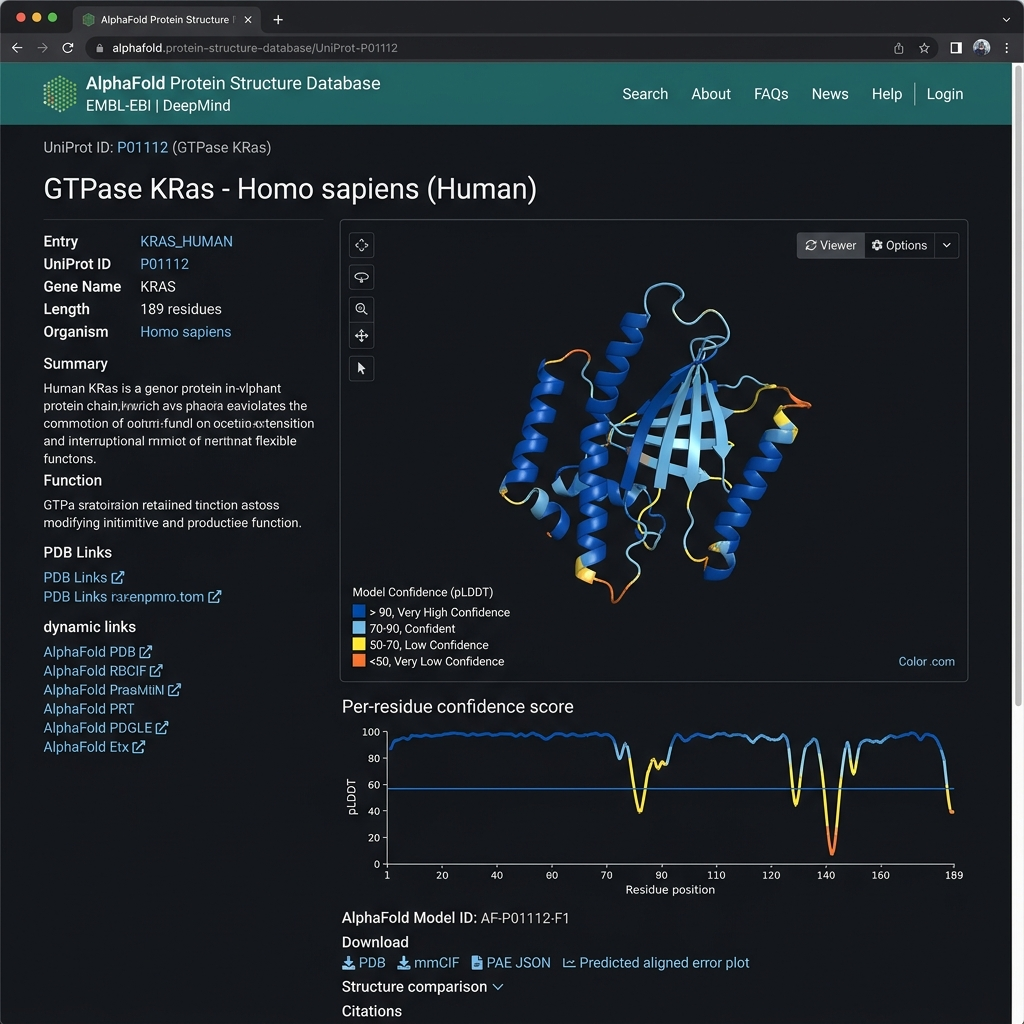
\includegraphics[width=0.82\linewidth]{images/alphafold_db_ui.jpg}
\caption[अल्फाफोल्ड प्रोटीन संरचना डेटाबेस]{अल्फाफोल्ड डेटाबेस (AlphaFold DB) का इंटरफ़ेस -- जहाँ मानव के KRas प्रोटीन (GTPase KRas) की 3D मुड़ी हुई संरचना और उसका स्थान-वार विश्वसनीयता ग्राफ़ (pLDDT score) दर्शाया गया है।}
\label{fig:alphafold-db-ui}
\end{figure}

\section{रोग-निदान में चित्र-पहचान}

जीव विज्ञान एवं चिकित्सा में बहुत-सी जानकारी \emph{चित्रों} के रूप में होती है - जैसे
X-ray, MRI, CT scan, या सूक्ष्मदर्शी (microscope) से ली गई कोशिकाओं की छवियाँ। AI इन
चित्रों में रोग के सूक्ष्म चिह्न पहचान सकती है, जिन्हें कभी-कभी आँख से देखना कठिन होता है।

\begin{itemize}[leftmargin=1.4em]
  \item \textbf{कैंसर-पहचान:} ऊतक (tissue) की छवियों में असामान्य कोशिकाएँ ढूँढना।
  \item \textbf{नेत्र-रोग:} रेटिना (retina) की तस्वीर से मधुमेह-जनित रोग पहचानना।
  \item \textbf{रक्त-जाँच:} सूक्ष्मदर्शी छवि में विभिन्न रक्त-कोशिकाओं की गिनती।
\end{itemize}

\noindent यहाँ ध्यान देने योग्य बात यह है कि AI डॉक्टर का \emph{स्थान} नहीं लेती; वह एक
\term{द्वितीय राय}{second opinion} देती है। अंतिम निर्णय सदैव चिकित्सक ही लेता है।

\begin{jante}
\textbf{भारतीय स्टार्टअप: रोग निदान में क्रांति (Indian Healthcare AI Startups):}
भारत में कई स्वास्थ्य-तकनीक (health-tech) कंपनियाँ चिकित्सा में AI के नवोन्मेषी अनुप्रयोग कर रही हैं। उदाहरण के लिए:
\begin{itemize}[leftmargin=1.2em]
  \item \textbf{Niramai:} यह बेंगलुरु आधारित कंपनी कृत्रिम बुद्धिमत्ता और थर्मल इमेजिंग (Thermal Imaging) का उपयोग करके बिना किसी दर्द या विकिरण (radiation) के बहुत ही प्रारंभिक चरण में स्तन कैंसर (Breast Cancer) की स्क्रीनिंग करती है।
  \item \textbf{Qure.ai:} यह मुंबई आधारित कंपनी AI का उपयोग करके चेस्ट एक्स-रे (Chest X-ray) और सीटी स्कैन का सेकंडों में विश्लेषण कर लेती है। इसका उपयोग सुदूर ग्रामीण क्षेत्रों में तपेदिक (Tuberculosis) और मस्तिष्क आघात (Brain Stroke) की तुरंत पहचान के लिए किया जा रहा है।
\end{itemize}
\end{jante}

\begin{gatividhi}[पत्तियों का वर्गीकरण - image classification]
\textbf{लक्ष्य:} यह अनुभव करना कि मशीन छवियों से प्रजातियाँ कैसे पहचानती है।\\[4pt]
\textbf{सामग्री:} कंप्यूटर/मोबाइल, वेबकैम, इंटरनेट।\\[4pt]
\textbf{चरण:}
\begin{enumerate}[leftmargin=1.6em]
  \item विद्यालय परिसर से 3 भिन्न पौधों की पत्तियाँ एकत्र करें।
  \item \emph{Teachable Machine} में तीन class बनाकर प्रत्येक पत्ती के 20-25 चित्र लें।
  \item मॉडल ``Train'' करें, फिर एक नई पत्ती दिखाकर परिणाम देखें।
  \item बताएँ - किन पत्तियों में मशीन सबसे अधिक भ्रमित (confused) हुई और क्यों?
\end{enumerate}
\textbf{अवलोकन:} समान दिखने वाली पत्तियों में मशीन की सटीकता (accuracy) घट जाती है -
ठीक वैसे ही जैसे मनुष्य भी भ्रमित हो सकता है।
\end{gatividhi}

\section{जैविक डेटा पर Python (एक झलक)}

DNA केवल अक्षरों की एक पंक्ति है, अतः कंप्यूटर उसे आसानी से पढ़ सकता है। नीचे का छोटा
Python कोड किसी DNA क्रम में चारों क्षारकों की गिनती करता है - यह \emph{Bioinformatics}
का सबसे आधारभूत कार्य है। (इसे चलाना अध्याय~5 में सीखेंगे।)

\begin{lstlisting}
# a short DNA sequence
dna = "ATGCGGATTACGCTAGCATGGC"

for base in "ATGC":
    print(base, "count =", dna.count(base))

# GC content - linked to several biological properties
gc = (dna.count("G") + dna.count("C")) / len(dna) * 100
print("GC content =", round(gc, 1), "%")
\end{lstlisting}
\colabnb{https://colab.research.google.com/github/kkreboot/ai-in-science-hindi/blob/main/notebooks/ch4-dna.ipynb}

\noindent यहाँ मशीन कोई जीव विज्ञान नहीं ``जानती''; वह केवल अक्षरों की गिनती कर रही है।
फिर भी यही सरल गिनती किसी जीन की पहचान में पहला कदम बन सकती है।

\section{प्रजाति-पहचान एवं जैव-विविधता}

AI अब क्षेत्र-जीव विज्ञान (field biology) में भी उपयोगी है। मोबाइल ऐप किसी पौधे, पक्षी
या कीट की तस्वीर से उसकी प्रजाति (species) पहचान सकते हैं। इससे विद्यार्थी एवं नागरिक
भी \term{नागरिक विज्ञान}{Citizen Science} में भाग ले सकते हैं और जैव-विविधता
(biodiversity) का डेटा एकत्र कर सकते हैं।

\begin{jante}
\emph{iNaturalist} एवं इसी प्रकार के ऐप करोड़ों तस्वीरों पर प्रशिक्षित हैं। जब आप कोई
तस्वीर डालते हैं, तो AI तुरंत सम्भावित प्रजातियों के नाम सुझा देती है - और यह डेटा
वैज्ञानिकों को प्रजातियों के फैलाव (distribution) का अध्ययन करने में मदद करता है।
\end{jante}

% ---------------- परियोजना ----------------
\begin{pariyojana}[स्थानीय जैव-विविधता का मानचित्र]
\textbf{उद्देश्य:} AI-आधारित प्रजाति-पहचान का उपयोग कर अपने क्षेत्र का जैव-विविधता
डेटा एकत्र करना और उसकी सीमाएँ समझना।\\[4pt]
\textbf{सामग्री:} मोबाइल कैमरा, \emph{iNaturalist} या ``Google Lens'' जैसा ऐप।\\[4pt]
\textbf{कार्य (समूह में, 3-4 विद्यार्थी):}
\begin{enumerate}[leftmargin=1.6em]
  \item दो सप्ताह तक अपने आस-पास के 15-20 पौधों/पक्षियों/कीटों की तस्वीरें लें।
  \item प्रत्येक के लिए ऐप द्वारा सुझाई गई प्रजाति नोट करें।
  \item जाँचें - किन मामलों में AI निश्चित (confident) थी और किनमें संदेह में?
        जहाँ सम्भव हो, किसी पुस्तक या शिक्षक से उत्तर सत्यापित करें।
  \item एक सरल तालिका/मानचित्र बनाएँ जिसमें प्रजाति, स्थान एवं AI की शुद्धता दर्शाई हो।
  \item निष्कर्ष लिखें - स्थानीय डेटा की कमी मॉडल की सटीकता को कैसे प्रभावित करती है?
\end{enumerate}
\textbf{मूल्यांकन:} एकत्र डेटा की विविधता, सत्यापन की गंभीरता एवं निष्कर्ष की
स्पष्टता के आधार पर।
\end{pariyojana}

% ---------------- सारांश ----------------
\section*{सारांश (Summary)}
\addcontentsline{toc}{section}{सारांश}
\begin{itemize}[leftmargin=1.4em]
  \item जीवन की जानकारी DNA में चार क्षारकों (A, T, G, C) के क्रम के रूप में एक विशाल
        डेटा है, जिसका विश्लेषण Bioinformatics में AI द्वारा होता है।
  \item AlphaFold ने प्रोटीन-वलन (protein folding) की दशकों पुरानी समस्या को AI से
        हल करने में बड़ी सफलता पाई।
  \item चिकित्सा-चित्रों में रोग-पहचान image classification का महत्वपूर्ण उपयोग है,
        जहाँ AI द्वितीय राय देती है पर निर्णय चिकित्सक का होता है।
  \item प्रजाति-पहचान ऐप नागरिक विज्ञान एवं जैव-विविधता अध्ययन को सरल बनाते हैं।
  \item DNA जैसे डेटा पर सरल Python से ही जैविक विश्लेषण आरम्भ किया जा सकता है।
\end{itemize}

% ---------------- अभ्यास ----------------
\section*{अभ्यास (Exercises)}
\addcontentsline{toc}{section}{अभ्यास}
\textbf{अ. रिक्त स्थान भरिए:}
\begin{enumerate}[leftmargin=1.6em]
  \item DNA चार क्षारकों \rule{2.8cm}{0.4pt} के क्रम से बनता है।
  \item प्रोटीन की 3D संरचना के पूर्वानुमान करने वाली प्रसिद्ध AI का नाम
        \rule{2.8cm}{0.4pt} है।
  \item जैविक डेटा के विश्लेषण के क्षेत्र को \rule{2.8cm}{0.4pt} कहते हैं।
\end{enumerate}

\textbf{ब. लघु उत्तरीय:}
\begin{enumerate}[leftmargin=1.6em]
  \item ``DNA एक डेटा है'' - इस कथन को समझाइए।
  \item चिकित्सा में AI ``डॉक्टर का स्थान नहीं लेती'' - इसका क्या अर्थ है?
  \item AlphaFold की उपलब्धि जीव विज्ञान के लिए क्यों महत्वपूर्ण है?
\end{enumerate}

\textbf{स. क्रियात्मक / दीर्घ उत्तरीय:}
\begin{enumerate}[leftmargin=1.6em]
  \item पत्तियों के वर्गीकरण वाली गतिविधि कीजिए तथा यह लिखिए कि चित्रों की संख्या
        बढ़ाने पर सटीकता पर क्या प्रभाव पड़ा।
  \item दिए गए DNA क्रम \texttt{ATGCATGC} में प्रत्येक क्षारक की गिनती कीजिए तथा
        GC content ज्ञात कीजिए।
  \item ``नागरिक विज्ञान में AI की भूमिका'' पर एक संक्षिप्त निबंध लिखिए।
\end{enumerate}

\begin{mcq}
  \item DNA में कितने प्रकार के क्षारक (bases) होते हैं?
    \begin{choices}\item 2 \item 3 \item 4 \item 5\end{choices}
  \item प्रोटीन की 3D संरचना का पूर्वानुमान करने वाला प्रसिद्ध AI तंत्र है:
    \begin{choices}\item AlphaFold \item AlphaGo \item DeepFace \item ChatGPT\end{choices}
  \item DNA क्रमों में पैटर्न खोजने वाला क्षेत्र कहलाता है:
    \begin{choices}\item जैव-सूचना विज्ञान (Bioinformatics) \item ज्योतिष
      \item भू-विज्ञान \item क्रिस्टलोग्राफी\end{choices}
  \item चिकित्सा-छवियों में रोग पहचानने में AI की भूमिका है:
    \begin{choices}\item डॉक्टर का स्थान लेना \item द्वितीय राय (second opinion) देना
      \item दवा बनाना \item शल्यक्रिया करना\end{choices}
\end{mcq}

\begin{mukhyashabd}
\textbf{क्षारक (bases: A,T,G,C)}, \textbf{जैव-सूचना विज्ञान (Bioinformatics)},
\textbf{प्रोटीन-वलन समस्या}, \textbf{AlphaFold}, \textbf{चित्र-वर्गीकरण (image classification)},
\textbf{द्वितीय राय (second opinion)}, \textbf{नागरिक विज्ञान (Citizen Science)},
\textbf{GC content}।
\end{mukhyashabd}
\selfcheckqr{https://forms.gle/aivigyan-ch4-quiz}

\chapter{Data, प्रयोग एवं AI उपकरण}
\label{ch:data}

\lakshyaheading
\begin{itemize}[leftmargin=1.4em]
  \item अच्छे data (good data) के गुण - शुद्धता, विविधता एवं पर्याप्त मात्रा।
  \item डेटा-विज्ञान (data science) के पाँच चरण - संग्रह से निष्कर्ष तक।
  \item data में \term{पक्षपात}{bias} को पहचानना एवं उससे बचना।
  \item विद्यार्थियों के लिए मुफ़्त एवं open-source AI उपकरण।
  \item \emph{Google Colab} में अपना पहला Python कोड स्वयं चलाना।
\end{itemize}

\section{``Garbage in, garbage out''}

कंप्यूटर विज्ञान का एक प्रसिद्ध कथन है - \emph{``Garbage in, garbage out''}, अर्थात्
यदि भीतर डाला गया data ख़राब है तो परिणाम भी ख़राब ही होगा। कोई भी AI उतनी ही अच्छी
होती है जितना उसका डेटा। इसीलिए वैज्ञानिक प्रयोग में data का \emph{सावधानीपूर्वक संग्रह}
सबसे महत्वपूर्ण चरण माना जाता है।

अच्छे data के तीन प्रमुख गुण हैं:
\begin{itemize}[leftmargin=1.4em]
  \item \term{शुद्धता}{Accuracy} - मान सही ढंग से एवं सही उपकरण से मापे गए हों।
  \item \term{विविधता}{Diversity} - data सभी प्रकार की स्थितियों को दर्शाता हो।
  \item \term{पर्याप्त मात्रा}{Sufficient quantity} - इतने उदाहरण हों कि pattern
        स्पष्ट दिखे।
\end{itemize}

\section{डेटा-विज्ञान के पाँच चरण}

किसी भी जाँच में - चाहे भौतिकी की हो, रसायन की या जीव विज्ञान की - data के साथ कार्य
प्रायः इन्हीं पाँच चरणों में होता है:

\begin{enumerate}[leftmargin=1.8em]
  \item \term{संग्रह}{Collection} - सेंसर, सर्वेक्षण या प्रयोग से data एकत्र करना।
  \item \term{सफ़ाई}{Cleaning} - त्रुटियाँ, दोहराव एवं रिक्त (missing) मान हटाना।
  \item \term{विश्लेषण}{Analysis} - ग्राफ़ एवं सांख्यिकी (statistics) से pattern देखना।
  \item \term{मॉडलन}{Modelling} - pattern से नियम/पूर्वानुमान निकालना (जैसे regression)।
  \item \term{निष्कर्ष}{Conclusion} - परिणाम की वैज्ञानिक व्याख्या एवं सत्यापन।
\end{enumerate}

ये पाँच चरण प्रायः एक \emph{चक्र (cycle)} की तरह दोहराए जाते हैं - निष्कर्ष से नए
प्रश्न उठते हैं और फिर नया संग्रह आरम्भ होता है (चित्र~\ref{fig:ds-cycle})।

\begin{figure}[h]
\centering
\begin{tikzpicture}[font=\sffamily\small,
    dstep/.style={draw=aiblue, thick, fill=ailite, circle, align=center,
      minimum size=1.9cm, inner sep=1pt},
    arr/.style={-{Stealth[length=2.6mm]}, thick, aigreen}]
  \def\R{3cm}
  \node[dstep] (s1) at (90:\R)  {संग्रह\\\footnotesize Collection};
  \node[dstep] (s2) at (18:\R)  {सफ़ाई\\\footnotesize Cleaning};
  \node[dstep] (s3) at (-54:\R) {विश्लेषण\\\footnotesize Analysis};
  \node[dstep] (s4) at (-126:\R){मॉडलन\\\footnotesize Modelling};
  \node[dstep] (s5) at (162:\R) {निष्कर्ष\\\footnotesize Conclusion};
  \draw[arr] (s1) to[bend left=12] (s2);
  \draw[arr] (s2) to[bend left=12] (s3);
  \draw[arr] (s3) to[bend left=12] (s4);
  \draw[arr] (s4) to[bend left=12] (s5);
  \draw[arr] (s5) to[bend left=12] (s1);
\end{tikzpicture}
\caption{डेटा-विज्ञान का चक्र: संग्रह से निष्कर्ष तक, और फिर नए प्रश्नों की ओर।}
\label{fig:ds-cycle}
\end{figure}

\begin{jante}
data वैज्ञानिक (data scientists) प्रायः अपना 60-80\% समय केवल \emph{चरण~2 (cleaning)}
में लगाते हैं। असली कौशल अक्सर ``साफ़ data'' बनाने में ही होता है, न कि केवल model चलाने में।
\end{jante}

\section{data में पक्षपात (Bias)}

यदि एकत्र किया गया data एकपक्षीय हो, तो AI के परिणाम भी \term{पक्षपाती}{biased} होंगे -
भले ही कोड बिल्कुल सही हो। उदाहरण के लिए, यदि किसी पत्ती-पहचान model को केवल हरी पत्तियों
के चित्र दिए जाएँ, तो वह सूखी या पीली पत्ती पहचानने में असफल रहेगा।

इसीलिए वैज्ञानिक कार्य में यह सदैव पूछा जाता है - ``क्या मेरा data सभी स्थितियों का
प्रतिनिधित्व करता है?'' यह प्रश्न आगे अध्याय~6 (नैतिकता) से भी गहराई से जुड़ा है।

\begin{sochiye}
मान लीजिए किसी कक्षा की ``औसत लम्बाई'' केवल खेल-दल (sports team) के विद्यार्थियों से
मापी जाए। यह माप पूरी कक्षा के लिए सही क्यों नहीं होगी? यह डेटा-पक्षपात का उदाहरण कैसे है?
\end{sochiye}

\section{विद्यार्थियों के लिए उपयोगी मुफ़्त उपकरण}

इस पुस्तक की सभी गतिविधियाँ निःशुल्क (free) एवं प्रायः open-source उपकरणों से की जा
सकती हैं:

\begin{table}[h]
\centering
\begin{tabular}{@{}p{3.6cm} p{9.4cm}@{}}
\toprule
\rowcolor{cvBlue}\hdc{उपकरण (tool)} & \hdc{उपयोग} \\
\midrule
\href{https://teachablemachine.withgoogle.com/}{Teachable Machine} & बिना कोड के image/sound classification \\
\href{https://colab.research.google.com/}{Google Colab}      & ब्राउज़र में मुफ़्त Python चलाना (कुछ इंस्टॉल नहीं करना पड़ता) \\
\href{https://phyphox.org/}{Phyphox}           & मोबाइल सेंसर से भौतिक data एकत्र करना \\
\href{https://orangedatamining.com/}{Orange Data Mining} & दृश्य (visual) रूप से ML समझना, बिना अधिक कोड \\
\href{https://molview.org/}{MolView} / \href{https://pubchem.ncbi.nlm.nih.gov/}{PubChem}  & अणुओं की 3D संरचना देखना \\
\bottomrule
\end{tabular}
\caption{इस पुस्तक में प्रयुक्त मुफ़्त एवं प्रायः open-source उपकरण (नाम पर क्लिक करने योग्य)}
\end{table}

\noindent\footnotesize\textcolor{aigrey}{सूचना: ऊपर तालिका में प्रत्येक उपकरण का नाम
क्लिक करने योग्य लिंक है; डिजिटल (PDF) संस्करण में सीधे वेबसाइट खुल जाएगी।}\normalsize

\section{अपना पहला Python कोड (Google Colab में)}

पिछले अध्यायों में हमने कई बार Python कोड देखा। अब उसे स्वयं चलाने का समय है। \emph{Google
Colab} एक मुफ़्त सेवा है जो ब्राउज़र में ही Python चला देती है - कंप्यूटर पर कुछ भी
इंस्टॉल करने की आवश्यकता नहीं।

\begin{gatividhi}[Colab में पहला कदम - data का ग्राफ़ एवं regression]
\textbf{लक्ष्य:} स्वयं Python चलाकर data पर सर्वोत्तम रेखा खींचना।\\[4pt]
\textbf{सामग्री:} कंप्यूटर/मोबाइल, इंटरनेट, एक Google खाता।\\[4pt]
\textbf{चरण:}
\begin{enumerate}[leftmargin=1.6em]
  \item ब्राउज़र में \texttt{colab.research.google.com} खोलें और ``New Notebook'' चुनें।
  \item नीचे दिया कोड एक cell में लिखें (या copy करें)।
  \item cell के बाएँ ``play'' बटन (या Shift+Enter) दबाकर कोड चलाएँ।
  \item ग्राफ़ एवं छपा हुआ (printed) मान देखें।
\end{enumerate}
\end{gatividhi}

\begin{center}
\fbox{\qrcode[height=2.2cm]{https://colab.research.google.com/}}\\[3pt]
{\footnotesize\sffamily\color{aigrey} Google Colab खोलने हेतु इस QR को स्कैन करें\\
(\nolinkurl{colab.research.google.com})}
\end{center}

\begin{lstlisting}
import numpy as np
import matplotlib.pyplot as plt

# experiment data (e.g. a spring: force vs extension)
x = np.array([0.02, 0.04, 0.06, 0.08, 0.10])
y = np.array([1.0, 2.1, 2.9, 4.2, 5.0])

# modelling: best-fit straight line y = m*x + c
m, c = np.polyfit(x, y, 1)
print("slope m =", round(m, 2), " intercept c =", round(c, 2))

# analysis: graph of the data and the fitted line
plt.scatter(x, y, label="data")          # original data points
plt.plot(x, m*x + c, color="red", label="best-fit line")
plt.xlabel("x"); plt.ylabel("y"); plt.legend()
plt.show()
\end{lstlisting}
\colabnb{https://colab.research.google.com/github/kkreboot/ai-in-science-hindi/blob/main/notebooks/ch5-regression-plot.ipynb}

\noindent यह वही \emph{least-squares regression} है जिसे आपने अध्याय~2 में हाथ से किया
था - अब कंप्यूटर इसे कुछ ही क्षणों में, अधिक सटीकता से कर देता है।

\begin{gatividhi}[कक्षा का data - सहसम्बन्ध (correlation)]
\textbf{लक्ष्य:} वास्तविक data एकत्र कर उसमें सम्बन्ध खोजना।\\[4pt]
\textbf{चरण:}
\begin{enumerate}[leftmargin=1.6em]
  \item पूरी कक्षा की लम्बाई (height) एवं भुजा-विस्तार (arm-span) मापें।
  \item दोनों का scatter-plot बनाएँ (कागज़ पर या Colab में)।
  \item देखें - क्या लम्बाई बढ़ने पर भुजा-विस्तार भी बढ़ता है (correlation)?
\end{enumerate}
\textbf{नोट:} यहाँ ``height'' एवं ``arm-span'' को ML की भाषा में \emph{feature} कहते हैं।
\end{gatividhi}

% ---------------- परियोजना ----------------
\begin{pariyojana}[अपना पहला डेटासेट - पूरा डेटा-विज्ञान चक्र]
\textbf{उद्देश्य:} किसी एक प्रश्न पर स्वयं data एकत्र कर पाँचों चरणों का पालन करना।\\[4pt]
\textbf{कार्य (समूह में, 3-4 विद्यार्थी):}
\begin{enumerate}[leftmargin=1.6em]
  \item एक प्रश्न चुनें - जैसे ``दिन के विभिन्न समय पर कक्षा का तापमान कैसे बदलता है?''
        या ``पौधे की वृद्धि प्रतिदिन कितनी होती है?''
  \item \textbf{संग्रह:} कम से कम एक सप्ताह नियमित रूप से मान मापें एवं तालिका में लिखें।
  \item \textbf{सफ़ाई:} ग़लत या छूटे हुए मानों को जाँचें एवं ठीक करें।
  \item \textbf{विश्लेषण:} data का ग्राफ़ बनाएँ (कागज़ या Colab)।
  \item \textbf{मॉडलन:} यदि सम्भव हो तो एक प्रवृत्ति-रेखा (trend line) खींचें एवं किसी
        अगले मान का पूर्वानुमान करें।
  \item \textbf{निष्कर्ष:} परिणाम को 5 स्लाइड या एक पोस्टर के रूप में प्रस्तुत करें,
        और data की किन्हीं सीमाओं (limitations) का उल्लेख करें।
\end{enumerate}
\textbf{मूल्यांकन:} पाँचों चरणों के पालन, data की गुणवत्ता एवं निष्कर्ष की स्पष्टता
के आधार पर।
\end{pariyojana}

% ---------------- सारांश ----------------
\begin{bharatai}
\textbf{UPI} जैसी डिजिटल भुगतान प्रणालियाँ प्रतिदिन करोड़ों लेन-देन पर AI से धोखाधड़ी
(fraud) तुरंत पकड़ती हैं - यह वास्तविक-समय (real-time) डेटा-विश्लेषण का बेहतरीन उदाहरण है।
\end{bharatai}

\section*{सारांश (Summary)}
\addcontentsline{toc}{section}{सारांश}
\begin{itemize}[leftmargin=1.4em]
  \item अच्छा data (शुद्ध, विविध एवं पर्याप्त) ही अच्छी AI की नींव है -
        ``garbage in, garbage out''।
  \item डेटा-विज्ञान के पाँच चरण हैं: संग्रह, सफ़ाई, विश्लेषण, मॉडलन एवं निष्कर्ष।
  \item एकपक्षीय data से पक्षपाती (biased) परिणाम मिलते हैं, चाहे कोड सही हो।
  \item Teachable Machine, Google Colab, Phyphox एवं Orange जैसे मुफ़्त उपकरणों से
        विद्यार्थी स्वयं AI का अनुभव कर सकते हैं।
  \item Google Colab में कुछ ही पंक्तियों के Python से data का ग्राफ़ एवं regression
        किया जा सकता है।
\end{itemize}

% ---------------- अभ्यास ----------------
\section*{अभ्यास (Exercises)}
\addcontentsline{toc}{section}{अभ्यास}
\textbf{अ. रिक्त स्थान भरिए:}
\begin{enumerate}[leftmargin=1.6em]
  \item ``Garbage in, \rule{2.8cm}{0.4pt} out'' - ख़राब data से ख़राब परिणाम।
  \item डेटा-विज्ञान का वह चरण जिसमें त्रुटियाँ हटाई जाती हैं, \rule{2.8cm}{0.4pt} कहलाता है।
  \item ब्राउज़र में मुफ़्त Python चलाने का उपकरण \rule{2.8cm}{0.4pt} है।
\end{enumerate}

\textbf{ब. लघु उत्तरीय:}
\begin{enumerate}[leftmargin=1.6em]
  \item अच्छे data के तीन गुण लिखिए।
  \item डेटा-विज्ञान के पाँच चरण क्रम से बताइए।
  \item डेटा-पक्षपात (bias) क्या है? एक उदाहरण दीजिए।
\end{enumerate}

\textbf{स. क्रियात्मक / दीर्घ उत्तरीय:}
\begin{enumerate}[leftmargin=1.6em]
  \item Google Colab में ऊपर दिया कोड चलाइए तथा प्राप्त ढलान $m$ एवं $c$ के मान लिखिए।
  \item कक्षा के height बनाम arm-span data का scatter-plot बनाइए और सम्बन्ध का वर्णन कीजिए।
  \item किसी एक प्रश्न पर सप्ताह-भर data एकत्र कर पाँचों चरणों की एक संक्षिप्त रिपोर्ट
        बनाइए।
\end{enumerate}

\begin{mcq}
  \item ``Garbage in, garbage out'' का अर्थ है:
    \begin{choices}\item तेज़ कंप्यूटर \item ख़राब data से ख़राब परिणाम
      \item मुफ़्त सॉफ़्टवेयर \item बड़ा model\end{choices}
  \item ब्राउज़र में निःशुल्क Python चलाने की सेवा है:
    \begin{choices}\item Google Colab \item MS Word \item Photoshop \item VLC\end{choices}
  \item मोबाइल सेंसर से भौतिक data एकत्र करने वाला ऐप है:
    \begin{choices}\item Phyphox \item Spotify \item WhatsApp \item Zoom\end{choices}
  \item data में किसी वर्ग का अनुचित कम/अधिक प्रतिनिधित्व कहलाता है:
    \begin{choices}\item पक्षपात (bias) \item सटीकता \item ढलान \item औसत\end{choices}
\end{mcq}

\begin{mukhyashabd}
\textbf{अच्छा data} (शुद्धता, विविधता, पर्याप्त मात्रा),
\textbf{पाँच चरण} (संग्रह, सफ़ाई, विश्लेषण, मॉडलन, निष्कर्ष),
\textbf{पक्षपात (bias)}, \textbf{अभिलक्षण (feature)}, \textbf{सहसम्बन्ध (correlation)}।
\end{mukhyashabd}
\selfcheckqr{https://kkreboot.github.io/ai-in-science-hindi/quiz/ch5.html}

\chapter{AI की नैतिकता एवं भविष्य}
\label{ch:ethics}

\lakshyaheading
\begin{itemize}[leftmargin=1.4em]
  \item AI की सीमाएँ - यह सदैव ``सही'' क्यों नहीं होती।
  \item data में पक्षपात (bias) एवं निजता (privacy) की समस्याएँ।
  \item विज्ञान में AI के उत्तरदायी (responsible) उपयोग के सिद्धांत।
  \item भविष्य के क्षेत्र, करियर (careers) एवं अवसर।
\end{itemize}

\section{AI सदा ``सही'' नहीं होती}

यह समझना अत्यंत आवश्यक है कि AI जादू नहीं है। वह केवल उतना ही ``जानती'' है जितना उसे
data से सिखाया गया है। इसी कारण AI कभी-कभी पूरे आत्मविश्वास के साथ \emph{ग़लत} उत्तर भी
दे देती है। विज्ञान में, जहाँ शुद्धता सर्वोपरि है, इसलिए AI के हर परिणाम की
\term{जाँच एवं पुनरावृत्ति}{verification \& reproducibility} अनिवार्य मानी जाती है।

\begin{itemize}[leftmargin=1.4em]
  \item AI केवल \emph{सहसम्बन्ध (correlation)} देख सकती है; \emph{कारण (causation)}
        सिद्ध करना वैज्ञानिक का कार्य है।
  \item AI का परिणाम तब तक स्वीकार नहीं किया जाता जब तक वह प्रयोग या स्वतंत्र विधि से
        सत्यापित न हो।
\end{itemize}

\begin{jante}
आधुनिक भाषा-आधारित AI कभी-कभी ऐसे ``तथ्य'' गढ़ देती है जो वास्तव में होते ही नहीं -
इसे \emph{hallucination} कहते हैं। इसीलिए किसी भी वैज्ञानिक दावे को मूल स्रोत
(original source) से जाँचना आवश्यक है।
\end{jante}

\section{data में पक्षपात (Bias)}

अध्याय~5 में हमने देखा कि एकपक्षीय data से पक्षपाती परिणाम मिलते हैं। यह केवल तकनीकी
समस्या नहीं, बल्कि एक \emph{नैतिक} समस्या भी है, क्योंकि पक्षपाती AI किसी वर्ग के साथ
अन्याय कर सकती है।

\begin{sochiye}
यदि किसी रोग-निदान AI को केवल एक ही आयु-वर्ग के रोगियों का data दिया जाए, तो वह अन्य
आयु के रोगियों पर अच्छा कार्य क्यों नहीं करेगी? ऐसी स्थिति में किसे हानि हो सकती है,
और इससे कैसे बचा जाए? चर्चा कीजिए।
\end{sochiye}

\section{निजता एवं उत्तरदायित्व (Privacy \& Responsibility)}

विज्ञान, विशेषकर चिकित्सा एवं जीव विज्ञान में, अक्सर व्यक्तिगत data (जैसे चिकित्सा-रिकॉर्ड
या DNA) का उपयोग होता है। ऐसे data की \term{निजता}{privacy} एवं सुरक्षा बनाए रखना
वैज्ञानिक का नैतिक उत्तरदायित्व है। data का उपयोग केवल अनुमति (consent) से एवं निर्धारित
उद्देश्य के लिए ही होना चाहिए।

\subsection{उत्तरदायी AI के सिद्धांत (Responsible AI)}
अनेक देशों एवं संस्थाओं ने अब AI के उपयोग हेतु कुछ साझा सिद्धांत अपनाए हैं:
\begin{itemize}[leftmargin=1.4em]
  \item \term{पारदर्शिता}{Transparency} - AI ने किसी निर्णय तक कैसे पहुँचा, यह
        समझाने योग्य हो।
  \item \term{निष्पक्षता}{Fairness} - किसी समूह के साथ पक्षपात न हो।
  \item \term{जवाबदेही}{Accountability} - परिणाम के लिए उत्तरदायी मनुष्य निर्धारित हो।
  \item \term{निजता}{Privacy} - व्यक्तिगत data सुरक्षित रहे।
\end{itemize}

इन चार स्तम्भों (pillars) पर ही उत्तरदायी AI टिकी होती है (चित्र~\ref{fig:responsible-ai})।

\begin{figure}[h]
\centering
\begin{tikzpicture}[font=\sffamily\small,
    pillar/.style={draw=aiblue, thick, fill=ailite, rounded corners,
      minimum width=2.7cm, minimum height=1.3cm, align=center, inner sep=3pt},
    top/.style={draw=aigreen, very thick, fill=aigreenL, rounded corners,
      minimum width=9.6cm, minimum height=1cm, align=center}]
  \node[top] (roof) {\bfseries उत्तरदायी AI (Responsible AI)};
  \node[pillar, below left=0.9cm and 2.4cm of roof.south] (p1)
      {पारदर्शिता\\\footnotesize Transparency};
  \node[pillar, right=0.3cm of p1] (p2) {निष्पक्षता\\\footnotesize Fairness};
  \node[pillar, right=0.3cm of p2] (p3) {जवाबदेही\\\footnotesize Accountability};
  \node[pillar, right=0.3cm of p3] (p4) {निजता\\\footnotesize Privacy};
  \foreach \p in {p1,p2,p3,p4}
    \draw[aigrey, thick] (\p.north) -- (\p.north |- roof.south);
\end{tikzpicture}
\caption{उत्तरदायी AI के चार स्तम्भ - पारदर्शिता, निष्पक्षता, जवाबदेही एवं निजता।}
\label{fig:responsible-ai}
\end{figure}

\begin{gatividhi}[किसी AI उपकरण की सीमाएँ खोजिए]
\textbf{लक्ष्य:} व्यावहारिक रूप से समझना कि AI कहाँ चूकती है।\\[4pt]
\textbf{चरण:}
\begin{enumerate}[leftmargin=1.6em]
  \item पिछले अध्यायों में बनाए किसी model (जैसे Teachable Machine का पत्ती-वर्गीकरण)
        को जानबूझकर कठिन उदाहरण दिखाएँ - जैसे कम रोशनी, उलटी या आधी ढकी वस्तु।
  \item नोट करें कि किन स्थितियों में model ग़लत या अनिश्चित (uncertain) हुआ।
  \item विचार करें - क्या इसका कारण data की कमी या पक्षपात था?
\end{enumerate}
\textbf{निष्कर्ष:} किसी भी AI को उपयोग करने से पहले उसकी सीमाएँ जानना आवश्यक है।
\end{gatividhi}

\section{भविष्य एवं करियर (Future \& Careers)}

AI एवं विज्ञान के संगम से अनेक नए एवं रोमांचक क्षेत्र बन रहे हैं:
\begin{itemize}[leftmargin=1.4em]
  \item \eterm{Bioinformatics} - जीव विज्ञान एवं data का मेल।
  \item \eterm{Computational Physics} - प्रयोग एवं सिमुलेशन।
  \item \eterm{Data Science} - हर क्षेत्र में data से निर्णय।
  \item चिकित्सा, कृषि (agriculture), मौसम एवं पर्यावरण में AI के अनुप्रयोग।
\end{itemize}

\noindent इन सभी क्षेत्रों का आधार वही विषय हैं जो आप अभी पढ़ रहे हैं - Physics,
Chemistry, Biology एवं Mathematics। इनकी मज़बूत समझ ही भविष्य में AI को सार्थक रूप से
उपयोग करने की कुंजी है।

\begin{jante}
भविष्य की अधिकांश वैज्ञानिक खोजें सम्भवतः मनुष्य एवं AI के \emph{सहयोग} से होंगी -
जहाँ AI विशाल data संभालेगी और मनुष्य कल्पना, प्रश्न एवं नैतिक निर्णय देगा।
\end{jante}

% ---------------- परियोजना ----------------
\begin{pariyojana}[वाद-विवाद - विज्ञान में निर्णय किसका?]
\textbf{उद्देश्य:} AI के नैतिक पहलुओं पर तर्कसंगत ढंग से सोचना एवं चर्चा करना।\\[4pt]
\textbf{विषय:} ``विज्ञान में महत्वपूर्ण निर्णय AI को सौंपे जाने चाहिए या नहीं।''\\[4pt]
\textbf{कार्य (पूरी कक्षा):}
\begin{enumerate}[leftmargin=1.6em]
  \item कक्षा को दो दलों में बाँटें - एक पक्ष में, एक विपक्ष में।
  \item प्रत्येक दल इस पुस्तक के उदाहरणों (AlphaFold, रोग-निदान, bias आदि) का उपयोग
        कर तथ्यों के साथ अपना पक्ष तैयार करे।
  \item बारी-बारी से तर्क प्रस्तुत करें; फिर खुली चर्चा करें।
  \item अंत में मिलकर एक \emph{संतुलित निष्कर्ष} लिखें - AI का उपयोग कब उचित है और
        मनुष्य की भूमिका कहाँ अनिवार्य है।
\end{enumerate}
\textbf{मूल्यांकन:} तर्कों की गुणवत्ता, उदाहरणों के उपयोग एवं निष्कर्ष के संतुलन के
आधार पर।
\end{pariyojana}

% ---------------- सारांश ----------------
\begin{bharatai}
\textbf{NITI Aayog} ने ``Responsible AI for All'' रणनीति प्रस्तुत की है, जो AI के
उपयोग में निष्पक्षता, पारदर्शिता एवं समावेशिता (inclusiveness) पर बल देती है।
\end{bharatai}

\section*{सारांश (Summary)}
\addcontentsline{toc}{section}{सारांश}
\begin{itemize}[leftmargin=1.4em]
  \item AI सदा सही नहीं होती; विज्ञान में उसके हर परिणाम की जाँच एवं सत्यापन आवश्यक है।
  \item AI केवल सहसम्बन्ध (correlation) देखती है; कारण (causation) सिद्ध करना मनुष्य का
        कार्य है।
  \item पक्षपात (bias) एवं निजता (privacy) AI की प्रमुख नैतिक चुनौतियाँ हैं।
  \item उत्तरदायी AI के चार स्तम्भ हैं - पारदर्शिता, निष्पक्षता, जवाबदेही एवं निजता।
  \item भविष्य मनुष्य एवं AI के सहयोग का है, जिसकी नींव Physics, Chemistry, Biology
        एवं Mathematics की समझ है।
\end{itemize}

% ---------------- अभ्यास ----------------
\section*{अभ्यास (Exercises)}
\addcontentsline{toc}{section}{अभ्यास}
\textbf{अ. रिक्त स्थान भरिए:}
\begin{enumerate}[leftmargin=1.6em]
  \item AI द्वारा गढ़े गए झूठे ``तथ्य'' को \rule{2.8cm}{0.4pt} कहते हैं।
  \item AI केवल \rule{2.8cm}{0.4pt} देखती है, जबकि कारण सिद्ध करना मनुष्य का कार्य है।
  \item उत्तरदायी AI का वह सिद्धांत जिसमें निर्णय की व्याख्या सम्भव हो,
        \rule{2.8cm}{0.4pt} कहलाता है।
\end{enumerate}

\textbf{ब. लघु उत्तरीय:}
\begin{enumerate}[leftmargin=1.6em]
  \item ``AI सदा सही नहीं होती'' - दो कारण देकर समझाइए।
  \item उत्तरदायी AI (Responsible AI) के चार सिद्धांत लिखिए।
  \item विज्ञान में डेटा-निजता क्यों महत्वपूर्ण है?
\end{enumerate}

\textbf{स. क्रियात्मक / दीर्घ उत्तरीय:}
\begin{enumerate}[leftmargin=1.6em]
  \item किसी model को कठिन उदाहरण दिखाकर उसकी सीमाएँ खोजने वाली गतिविधि कीजिए और
        अपने अवलोकन लिखिए।
  \item ``विज्ञान में AI - वरदान या चुनौती'' विषय पर एक निबंध लिखिए।
  \item आप भविष्य में AI से जुड़ा कौन-सा वैज्ञानिक क्षेत्र चुनना चाहेंगे, और क्यों?
\end{enumerate}

\begin{mcq}
  \item AI द्वारा आत्मविश्वास से दिया गया ग़लत उत्तर कहलाता है:
    \begin{choices}\item मतिभ्रम (hallucination) \item पक्षपात
      \item समाश्रयण \item प्रशिक्षण\end{choices}
  \item निर्णय की व्याख्या सम्भव होने का सिद्धांत है:
    \begin{choices}\item पारदर्शिता (transparency) \item गोपनीयता
      \item गति \item संपीडन\end{choices}
  \item निम्न में से कौन \emph{उत्तरदायी AI} का सिद्धांत नहीं है?
    \begin{choices}\item निष्पक्षता \item जवाबदेही
      \item डेटा-चोरी \item निजता\end{choices}
  \item विज्ञान में अंतिम निर्णय किसके पास रहना चाहिए?
    \begin{choices}\item AI model \item मनुष्य (वैज्ञानिक)
      \item कंप्यूटर \item इंटरनेट\end{choices}
\end{mcq}

\begin{mukhyashabd}
\textbf{मतिभ्रम (Hallucination)}, \textbf{सहसम्बन्ध बनाम कारण (correlation vs causation)},
\textbf{पक्षपात (bias)}, \textbf{निजता (privacy)}, \textbf{उत्तरदायी AI} -
पारदर्शिता, निष्पक्षता, जवाबदेही, निजता।
\end{mukhyashabd}
\selfcheckqr{https://kkreboot.github.io/ai-in-science-hindi/quiz/ch6.html}

% ============================================================
%  पुस्तक का समापन (closing)
% ============================================================
\section*{आगे की राह (The Road Ahead)}
\addcontentsline{toc}{section}{आगे की राह}

इस पुस्तक में हमने देखा कि कृत्रिम बुद्धिमत्ता कोई अलग ``जादुई'' विषय नहीं, बल्कि
विज्ञान को देखने का एक नया दृष्टिकोण है - जहाँ हर प्रयोग, हर मापन एवं हर खोज के पीछे
\emph{data} है। भौतिकी में pattern, रसायन में अणु, और जीव विज्ञान में DNA - सभी को AI
data के रूप में ``पढ़'' सकती है।

परन्तु सबसे महत्वपूर्ण बात यह है कि AI एक \emph{उपकरण} है, वैज्ञानिक नहीं। जिज्ञासा,
कल्पना, प्रश्न पूछने की कला एवं नैतिक निर्णय - ये सदैव मनुष्य के पास रहेंगे। यदि यह
पुस्तक आपके मन में विज्ञान एवं AI के प्रति एक नई जिज्ञासा जगा सकी, तो इसका उद्देश्य
पूर्ण हुआ।

\begin{center}
\vspace{0.5em}
{\sffamily\bfseries\color{aiblue} सीखते रहिए, प्रयोग करते रहिए, प्रश्न पूछते रहिए।}\\[4pt]
\textit{- पुस्तक समाप्त -}
\end{center}


% ---------------- परिशिष्ट ----------------
\chapter*{शब्दावली (Glossary)}
\addcontentsline{toc}{chapter}{शब्दावली (Glossary)}
\markboth{शब्दावली}{शब्दावली}

इस पुस्तक में प्रयुक्त प्रमुख वैज्ञानिक एवं तकनीकी शब्दों का संक्षिप्त अर्थ नीचे
अंग्रेज़ी वर्णक्रम (alphabetical order) में दिया गया है।

\begin{longtable}{@{}p{5.2cm} p{8.3cm}@{}}
\toprule
\rowcolor{cvBlue}\hdc{शब्द (Term)} & \hdc{अर्थ (Meaning)} \\
\midrule
\endfirsthead
\toprule
\rowcolor{cvBlue}\hdc{शब्द (Term)} & \hdc{अर्थ (Meaning)} \\
\midrule
\endhead
\bottomrule
\multicolumn{2}{r}{\small\itshape अगले पृष्ठ पर जारी \dots} \\
\endfoot
\bottomrule
\endlastfoot

\textbf{Accountability} (जवाबदेही) & किसी AI-निर्णय के परिणाम के लिए उत्तरदायी मनुष्य का निर्धारण। \\
\textbf{Accuracy} (शुद्धता) & माप या पूर्वानुमान का सही मान के कितना निकट होना। \\
\textbf{AI} (कृत्रिम बुद्धिमत्ता) & मशीनों द्वारा मानव-जैसे बौद्धिक कार्य करना। देखें Artificial Intelligence। \\
\textbf{AlphaFold} & DeepMind की वह AI जिसने प्रोटीन की 3D संरचना का पूर्वानुमान किया (2021)। \\
\textbf{Analysis} (विश्लेषण) & ग्राफ़ एवं सांख्यिकी द्वारा data में pattern देखना (डेटा-विज्ञान का चरण~3)। \\
\textbf{Artificial Intelligence} (कृत्रिम बुद्धिमत्ता) & मशीनों द्वारा देखना, सीखना, तर्क एवं निर्णय जैसे बौद्धिक कार्य करना। \\
\textbf{Bases} (क्षारक) & DNA के चार “अक्षर” - A, T, G, C। \\
\textbf{Bias} (पक्षपात) & एकपक्षीय data के कारण AI के झुके हुए या अनुचित परिणाम। \\
\textbf{Bioinformatics} (जैव-सूचना विज्ञान) & जैविक data (DNA, प्रोटीन) का कंप्यूटर द्वारा विश्लेषण। \\
\textbf{Catalyst} (उत्प्रेरक) & वह पदार्थ जो अभिक्रिया की दर बढ़ाता है; AI नए उत्प्रेरक खोजने में सहायक। \\
\textbf{Causation} (कारण-सम्बन्ध) & एक घटना का दूसरी घटना का वास्तविक कारण होना (केवल correlation से भिन्न)। \\
\textbf{Citizen Science} (नागरिक विज्ञान) & आम नागरिकों द्वारा वैज्ञानिक data एकत्र करना। \\
\textbf{Classification} (वर्गीकरण) & वस्तुओं या data को श्रेणियों में बाँटना (जैसे अम्ल/क्षार)। \\
\textbf{Cleaning} (सफ़ाई) & data से त्रुटियाँ, दोहराव एवं रिक्त मान हटाना (चरण~2)। \\
\textbf{Collection} (संग्रह) & प्रयोग, सेंसर या सर्वेक्षण से data एकत्र करना (चरण~1)। \\
\textbf{Computational Physics} (संगणनात्मक भौतिकी) & कंप्यूटर-सिमुलेशन एवं data द्वारा भौतिकी का अध्ययन। \\
\textbf{Conclusion} (निष्कर्ष) & परिणाम की वैज्ञानिक व्याख्या एवं सत्यापन (चरण~5)। \\
\textbf{Correlation} (सहसम्बन्ध) & दो राशियों का साथ-साथ बदलना (कारण होना आवश्यक नहीं)। \\
\textbf{Data} (data) & मापे गए मानों या जानकारी का संग्रह। \\
\textbf{Data Science} (data विज्ञान) & data से ज्ञान एवं निर्णय निकालने का विज्ञान। \\
\textbf{Decision} (निर्णय) & उपलब्ध विकल्पों में से सर्वोत्तम चुनना। \\
\textbf{Deep Learning} (गहन अधिगम) & अनेक परतों वाले neural network पर आधारित ML। \\
\textbf{Diversity} (विविधता) & data का सभी प्रकार की स्थितियों का प्रतिनिधित्व करना। \\
\textbf{Error} (त्रुटि) & मापे गए एवं वास्तविक मान का अंतर। \\
\textbf{Fairness} (निष्पक्षता) & AI द्वारा किसी समूह के साथ पक्षपात न होना। \\
\textbf{Feature} (अभिलक्षण) & data का वह गुण जिस पर model आधारित होता है (जैसे height)। \\
\textbf{GC content} (जी-सी अनुपात) & DNA में G एवं C क्षारकों का प्रतिशत; कई जैविक गुणों से जुड़ा। \\
\textbf{General AI} (सामान्य AI) & मनुष्य-जैसी सर्व-कार्य बुद्धि (अभी केवल शोध का विषय)। \\
\textbf{Hallucination} (मतिभ्रम) & AI द्वारा गढ़ा गया झूठा “तथ्य” जो वास्तव में नहीं होता। \\
\textbf{Large Hadron Collider} (वृहत् हैड्रॉन संघट्टक, LHC) & CERN का विशाल कण-त्वरक जो प्रति सेकंड लगभग एक अरब टकराव करता है। \\
\textbf{Law} (नियम) & प्रकृति के व्यवहार का सामान्य एवं परीक्षित कथन। \\
\textbf{Learning} (अधिगम) & उदाहरणों से नियम या pattern सीखना। \\
\textbf{Least Squares Method} (अल्पतम वर्ग विधि) & त्रुटि का वर्ग न्यूनतम कर सर्वोत्तम रेखा खोजना। \\
\textbf{Machine Learning} (मशीन लर्निंग, ML) & data से स्वयं नियम सीखने वाली AI; AI का एक भाग। \\
\textbf{Modelling} (मॉडलन) & pattern से नियम या पूर्वानुमान बनाना (चरण~4)। \\
\textbf{Molecule Design} (अणु-अभिकल्प) & वांछित गुण वाले नए अणु AI द्वारा सुझाना। \\
\textbf{Narrow AI} (सँकरी AI) & केवल एक कार्य में निपुण AI; आज की लगभग सारी AI इसी प्रकार की। \\
\textbf{Neural Network} (तंत्रिका नेटवर्क) & मस्तिष्क की कोशिकाओं से प्रेरित एक ML model। \\
\textbf{Pattern} (pattern) & data में दिखने वाली नियमितता या रुझान। \\
\textbf{Perception} (प्रत्यक्षण) & चित्र, ध्वनि या सेंसर से जानकारी ग्रहण करना। \\
\textbf{Prediction} (पूर्वानुमान) & ज्ञात data से किसी अनदेखे मान का अनुमान। \\
\textbf{Privacy} (निजता) & व्यक्तिगत data की सुरक्षा एवं गोपनीयता। \\
\textbf{Property Prediction} (गुण-पूर्वानुमान) & अणु या पदार्थ के गुण (जैसे विषाक्तता) पहले से आँकना। \\
\textbf{Protein Folding Problem} (प्रोटीन-वलन समस्या) & अमीनो-अम्ल क्रम से प्रोटीन की 3D संरचना का पूर्वानुमान। \\
\textbf{Random Error} (यादृच्छिक त्रुटि) & हर बार बदलती हुई त्रुटि (जैसे प्रतिक्रिया-समय)। \\
\textbf{Reasoning} (तर्क) & उपलब्ध जानकारी से निष्कर्ष निकालना। \\
\textbf{Regression} (समाश्रयण) & data पर सर्वोत्तम रेखा या वक्र फिट करना। \\
\textbf{Reproducibility} (पुनरावृत्ति) & किसी परिणाम का दोबारा दोहराया जा सकना। \\
\textbf{Responsible AI} (उत्तरदायी AI) & पारदर्शिता, निष्पक्षता, जवाबदेही एवं निजता के साथ AI का उपयोग। \\
\textbf{Second Opinion} (द्वितीय राय) & निर्णय की पुष्टि हेतु एक अतिरिक्त राय (जैसे रोग-निदान में AI)। \\
\textbf{SMILES} (स्माइल्स संकेतन) & अणु को एक पंक्ति (string) के रूप में लिखने की विधि। \\
\textbf{Sufficient Quantity} (पर्याप्त मात्रा) & pattern स्पष्ट दिखने योग्य data की मात्रा। \\
\textbf{Systematic Error} (क्रमबद्ध त्रुटि) & हर बार एक ही दिशा में होने वाली त्रुटि। \\
\textbf{Training Data} (प्रशिक्षण data) & model को सिखाने हेतु दिए गए उदाहरण। \\
\textbf{Transparency} (पारदर्शिता) & AI के किसी निर्णय की व्याख्या कर पाने की योग्यता। \\
\textbf{Virtual Screening} (आभासी छँटाई) & कंप्यूटर पर ही लाखों अणुओं को जाँचकर सम्भावित दवाएँ छाँटना। \\
\end{longtable}

\chapter*{उत्तर-कुंजी (Answer Key)}
\addcontentsline{toc}{chapter}{उत्तर-कुंजी (Answer Key)}
\markboth{उत्तर-कुंजी}{उत्तर-कुंजी}

यहाँ \textbf{अ (रिक्त स्थान)} एवं \textbf{ब (लघु उत्तरीय)} के उत्तर दिए गए हैं। \textbf{स}
भाग के अधिकांश प्रश्न गतिविधि एवं विचार आधारित हैं, अतः उनके लिए केवल \emph{संकेत/आदर्श
बिंदु} दिए गए हैं - विद्यार्थियों के उत्तर भिन्न हो सकते हैं।

% ---------------- अध्याय 1 ----------------
\section*{अध्याय 1: कृत्रिम बुद्धिमत्ता का परिचय}
\textbf{अ.} 1. Machine Learning (मशीन लर्निंग) \quad 2. Narrow (सँकरी) AI

\noindent\textbf{ब.}
\begin{enumerate}[leftmargin=1.6em]
  \item परम्परागत प्रोग्राम को \emph{नियम + डेटा} दिए जाते हैं और वह नियम लागू करता है;
        ML को \emph{डेटा + उत्तर} दिए जाते हैं और वह नियम स्वयं खोजती है। उदाहरण -
        कैलकुलेटर (परम्परागत) बनाम चेहरा-पहचान (ML)।
  \item विज्ञान में आज डेटा बहुत विशाल है; AI उसे (i) तेज़ी से, (ii) धैर्यपूर्वक तथा
        (iii) बड़े पैमाने (scale) पर विश्लेषित कर ऐसे पैटर्न पकड़ लेती है जो मनुष्य से
        छूट सकते हैं।
\end{enumerate}

\noindent\textbf{स.} \textit{(गतिविधि)} सामान्यतः class बढ़ाने पर, समान मात्रा में
डेटा हो तो accuracy कुछ घट सकती है; अधिक एवं विविध चित्र देने पर सुधरती है।

% ---------------- अध्याय 2 ----------------
\section*{अध्याय 2: भौतिकी में कृत्रिम बुद्धिमत्ता}
\textbf{अ.} 1. रैखिक समाश्रयण / Linear Regression (Least Squares) \quad
2. दूरी/त्रुटि (error) \quad 3. क्रमबद्ध (Systematic) त्रुटि

\noindent\textbf{ब.}
\begin{enumerate}[leftmargin=1.6em]
  \item गैलीलियो ने झुके तल पर गेंद के समय एवं दूरी का \emph{डेटा} लेकर पैटर्न
        ($s \propto t^2$) खोजा - अर्थात् भौतिकी का नियम डेटा में पैटर्न खोजने से ही मिला।
  \item regression डेटा-बिंदुओं के बीच सर्वोत्तम रेखा खोजता है; उसकी ढलान ही नियम का
        स्थिरांक होती है। जैसे बल बनाम विस्तार के डेटा से ढलान = स्प्रिंग नियतांक $k$
        ($F = kx$)।
  \item LHC प्रति सेकंड लगभग एक अरब टकराव एवं भारी डेटा बनाता है; इनमें से दुर्लभ
        महत्वपूर्ण घटनाएँ छाँटना केवल AI से ही सम्भव है।
\end{enumerate}

\noindent\textbf{स.}
\begin{enumerate}[leftmargin=1.6em]
  \item \textit{(गतिविधि)} बल बनाम विस्तार की सर्वोत्तम रेखा की ढलान ही $k$ है।
  \item $m = 2,\; c = 0$; सम्बन्ध $y = 2x$ अर्थात् $y$, $x$ के अनुक्रमानुपाती - जैसे
        हुक का नियम $F = kx$।
  \item \textit{(गतिविधि)} त्वरण-ग्राफ़ प्रायः आवर्ती (periodic) दिखता है; उत्तर
        एकत्र डेटा पर निर्भर।
\end{enumerate}

% ---------------- अध्याय 3 ----------------
\section*{अध्याय 3: रसायन विज्ञान में कृत्रिम बुद्धिमत्ता}
\textbf{अ.} 1. SMILES (स्माइल्स संकेतन) \quad 2. वर्गीकरण (classification) \quad
3. आभासी छँटाई (Virtual Screening)

\noindent\textbf{ब.}
\begin{enumerate}[leftmargin=1.6em]
  \item मेंडेलीफ़ ने ज्ञात तत्वों की \emph{प्रवृत्ति (trend/pattern)} देखकर अनदेखे
        तत्वों के गुणों का पूर्वानुमान किया - ML भी ज्ञात डेटा के पैटर्न से अनदेखे मान
        का पूर्वानुमान करता है।
  \item classification में वस्तु को श्रेणी में बाँटा जाता है (जैसे अम्ल/क्षार);
        prediction में कोई सतत मान आँका जाता है (जैसे क्वथनांक)।
  \item (i) आभासी छँटाई (virtual screening), (ii) गुण/विषाक्तता-पूर्वानुमान, तथा
        (iii) नए अणुओं का अभिकल्प (molecule design)।
\end{enumerate}

\noindent\textbf{स.} \textit{(गतिविधि)} आवर्त में बाएँ से दाएँ त्रिज्या घटती है; 1.
पूर्वानुमान-त्रुटि छोटी आनी चाहिए। 2. MolView से SMILES लिखें (जैसे एथेनॉल = \texttt{CCO})।
3. निबंध - virtual screening एवं गुण-पूर्वानुमान से समय व लागत घटती है (जैसे Halicin)।

% ---------------- अध्याय 4 ----------------
\section*{अध्याय 4: जीव विज्ञान में कृत्रिम बुद्धिमत्ता}
\textbf{अ.} 1. A, T, G, C \quad 2. AlphaFold \quad 3. Bioinformatics (जैव-सूचना विज्ञान)

\noindent\textbf{ब.}
\begin{enumerate}[leftmargin=1.6em]
  \item DNA केवल चार अक्षरों (A, T, G, C) के क्रम से बना एक विशाल अनुक्रम है, जिसे
        कंप्यूटर पढ़ एवं विश्लेषित कर सकता है - इसीलिए यह एक ``डेटा'' है।
  \item AI चित्रों में रोग के सूक्ष्म चिह्न दिखाकर एक \emph{द्वितीय राय (second
        opinion)} देती है, परन्तु अंतिम निर्णय सदैव चिकित्सक का होता है।
  \item AlphaFold ने प्रोटीन-वलन (protein folding) की दशकों पुरानी समस्या हल की,
        जिससे नई दवाओं एवं एंज़ाइमों की खोज बहुत तेज़ हो गई।
\end{enumerate}

\noindent\textbf{स.}
\begin{enumerate}[leftmargin=1.6em]
  \item \textit{(गतिविधि)} अधिक एवं विविध चित्र देने पर सटीकता (accuracy) बढ़ती है।
  \item \texttt{ATGCATGC} में A = 2, T = 2, G = 2, C = 2; \;
        GC content $= \dfrac{2+2}{8}\times 100 = 50\%$।
  \item \textit{(निबंध)} ऐप करोड़ों तस्वीरों पर प्रशिक्षित होकर प्रजाति पहचानते हैं;
        नागरिक डेटा-संग्रह में भाग ले सकते हैं।
\end{enumerate}

% ---------------- अध्याय 5 ----------------
\section*{अध्याय 5: डेटा, प्रयोग एवं AI उपकरण}
\textbf{अ.} 1. garbage \quad 2. सफ़ाई (Cleaning) \quad 3. Google Colab

\noindent\textbf{ब.}
\begin{enumerate}[leftmargin=1.6em]
  \item शुद्धता (accuracy), विविधता (diversity) एवं पर्याप्त मात्रा (sufficient
        quantity)।
  \item संग्रह $\to$ सफ़ाई $\to$ विश्लेषण $\to$ मॉडलन $\to$ निष्कर्ष।
  \item पक्षपात (bias) तब होता है जब डेटा एकपक्षीय हो और परिणाम झुक जाएँ - जैसे केवल
        खेल-दल से मापी गई ``औसत लम्बाई'' पूरी कक्षा के लिए ग़लत होगी।
\end{enumerate}

\noindent\textbf{स.}
\begin{enumerate}[leftmargin=1.6em]
  \item \textit{(गतिविधि)} दिए गए डेटा पर लगभग $m \approx 50.5,\; c \approx 0.01$
        प्राप्त होगा (मान थोड़े भिन्न हो सकते हैं)।
  \item \textit{(गतिविधि)} सामान्यतः धनात्मक सहसम्बन्ध (positive correlation) -
        लम्बाई बढ़ने पर भुजा-विस्तार भी बढ़ता है।
  \item \textit{(रिपोर्ट)} पाँचों चरणों का पालन एवं डेटा की सीमाओं का उल्लेख अपेक्षित।
\end{enumerate}

% ---------------- अध्याय 6 ----------------
\section*{अध्याय 6: AI की नैतिकता एवं भविष्य}
\textbf{अ.} 1. hallucination (मतिभ्रम) \quad 2. सहसम्बन्ध (correlation) \quad
3. पारदर्शिता (Transparency)

\noindent\textbf{ब.}
\begin{enumerate}[leftmargin=1.6em]
  \item AI केवल अपने प्रशिक्षण-डेटा जितना ही ``जानती'' है और कभी-कभी पूरे आत्मविश्वास
        से ग़लत/गढ़ा हुआ (hallucinated) उत्तर देती है; साथ ही वह केवल सहसम्बन्ध देखती
        है, कारण नहीं।
  \item पारदर्शिता (Transparency), निष्पक्षता (Fairness), जवाबदेही (Accountability)
        एवं निजता (Privacy)।
  \item चिकित्सा/जीव विज्ञान में व्यक्तिगत डेटा (जैसे चिकित्सा-रिकॉर्ड, DNA) प्रयोग
        होता है; उसकी सुरक्षा एवं केवल अनुमति से उपयोग वैज्ञानिक का नैतिक उत्तरदायित्व है।
\end{enumerate}

\noindent\textbf{स.} \textit{(गतिविधि/निबंध)} 1. कठिन उदाहरणों (कम रोशनी, उलटी वस्तु)
पर मॉडल की चूक देखें। 2-3. संतुलित दृष्टिकोण अपेक्षित - AI एक उपकरण है, अंतिम निर्णय
एवं नैतिक उत्तरदायित्व मनुष्य का।

% ---------------- बहुविकल्पीय उत्तर ----------------
\section*{बहुविकल्पीय प्रश्नों के उत्तर (MCQ Answers)}
\noindent
\textbf{अध्याय 1:} 1.~(A) \quad 2.~(B) \quad 3.~(B) \quad 4.~(C)\\
\textbf{अध्याय 2:} 1.~(B) \quad 2.~(B) \quad 3.~(A) \quad 4.~(A)\\
\textbf{अध्याय 3:} 1.~(A) \quad 2.~(B) \quad 3.~(A) \quad 4.~(B)\\
\textbf{अध्याय 4:} 1.~(C) \quad 2.~(A) \quad 3.~(A) \quad 4.~(B)\\
\textbf{अध्याय 5:} 1.~(B) \quad 2.~(A) \quad 3.~(A) \quad 4.~(A)\\
\textbf{अध्याय 6:} 1.~(A) \quad 2.~(A) \quad 3.~(C) \quad 4.~(B)

% ============================================================
%  परिशिष्ट ग : सन्दर्भ एवं अग्रिम पठन (References & Further Reading)
% ============================================================
\chapter*{परिशिष्ट ग: सन्दर्भ एवं अग्रिम पठन}
\addcontentsline{toc}{chapter}{परिशिष्ट ग: सन्दर्भ एवं अग्रिम पठन}
\markboth{सन्दर्भ एवं अग्रिम पठन}{सन्दर्भ एवं अग्रिम पठन}

\noindent नीचे विश्वसनीय एवं निःशुल्क स्रोतों की सूची दी गई है, जिनसे विद्यार्थी इस
पुस्तक के विषयों को और गहराई से समझ सकते हैं। (सभी लिंक पर क्लिक किया जा सकता है।)

\section*{सामान्य परिचय (General Introduction to AI)}
\begin{itemize}[leftmargin=1.4em]
  \item \href{https://www.elementsofai.com/}{Elements of AI} -- निःशुल्क ऑनलाइन
        पाठ्यक्रम (free online course), University of Helsinki.
  \item \href{https://www.youtube.com/watch?v=aircAruvnKK}{3Blue1Brown: Neural
        Networks} -- तंत्रिका जाल का दृश्य परिचय (visual introduction).
  \item \href{https://ai.google/education/}{Google AI Education} -- AI एवं ML
        सीखने हेतु सामग्री।
\end{itemize}

\section*{निःशुल्क उपकरण (Free Hands-on Tools)}
\begin{itemize}[leftmargin=1.4em]
  \item \href{https://teachablemachine.withgoogle.com/}{Teachable Machine} --
        बिना कोड के image/sound classification.
  \item \href{https://colab.research.google.com/}{Google Colab} -- ब्राउज़र में
        निःशुल्क Python.
  \item \href{https://phyphox.org/}{Phyphox} -- मोबाइल सेंसर से भौतिक डेटा।
  \item \href{https://orangedatamining.com/}{Orange Data Mining} -- दृश्य रूप से
        ML समझना।
  \item \href{https://molview.org/}{MolView} -- अणुओं की 3D संरचना।
\end{itemize}

\section*{विषयवार स्रोत (Subject-wise Sources)}
\begin{itemize}[leftmargin=1.4em]
  \item \textbf{भौतिकी:} \href{https://home.cern/}{CERN} एवं
        \href{https://www.nasa.gov/}{NASA} -- कण भौतिकी एवं खगोल में डेटा-विज्ञान।
  \item \textbf{रसायन:} \href{https://pubchem.ncbi.nlm.nih.gov/}{PubChem} --
        रासायनिक यौगिकों का खुला डेटाबेस।
  \item \textbf{जीव विज्ञान:} \href{https://alphafold.ebi.ac.uk/}{AlphaFold
        Protein Structure Database} एवं
        \href{https://www.ncbi.nlm.nih.gov/}{NCBI} -- प्रोटीन एवं जीनोम डेटा।
  \item \textbf{डेटा-विज्ञान:} \href{https://numpy.org/}{NumPy} एवं
        \href{https://matplotlib.org/}{Matplotlib} -- Python पुस्तकालय।
\end{itemize}

\begin{padhe}
इन स्रोतों का उपयोग करते समय \emph{स्रोत की विश्वसनीयता} (credibility) अवश्य जाँचें।
सरकारी, विश्वविद्यालयी एवं प्रतिष्ठित वैज्ञानिक संस्थाओं की वेबसाइट सामान्यतः अधिक
विश्वसनीय होती हैं। AI से प्राप्त उत्तर को भी किसी विश्वसनीय स्रोत से सत्यापित करें।
\end{padhe}

\section*{चित्र-आभार (Image Credits)}
\noindent इस पुस्तक में प्रयुक्त छायाचित्र \emph{सार्वजनिक डोमेन} (Public Domain) से लिए
गए हैं तथा Wikimedia Commons के सौजन्य से उपलब्ध हैं:
\begin{itemize}[leftmargin=1.4em]
  \item \textbf{चित्र~\ref{fig:hubble}} (हबल अल्ट्रा डीप फ़ील्ड): NASA \& ESA --
        Public Domain;
        \href{https://commons.wikimedia.org/wiki/File:Hubble_ultra_deep_field.jpg}{Wikimedia Commons}.
  \item \textbf{चित्र~\ref{fig:caffeine}} (कैफ़ीन अणु): Public Domain;
        \href{https://commons.wikimedia.org/wiki/File:Caffeine-3D-balls.png}{Wikimedia Commons}.
  \item \textbf{चित्र~\ref{fig:aspirin}} (एस्पिरिन अणु): Benjah-bmm27 -- Public
        Domain; \href{https://commons.wikimedia.org/wiki/File:Aspirin-3D-balls.png}{Wikimedia Commons}.
  \item \textbf{चित्र~\ref{fig:dna}} (DNA द्विकुंडलिनी): Forluvoft -- Public
        Domain; \href{https://commons.wikimedia.org/wiki/File:DNA_simple2.svg}{Wikimedia Commons}.
\end{itemize}
\noindent अन्य सभी आरेख (diagrams) लेखक द्वारा \emph{TikZ} में मूल रूप से बनाए गए हैं।

% ============================================================
%  परिशिष्ट घ: परियोजना मूल्यांकन रूब्रिक (Project Assessment Rubrics)
% ============================================================
\chapter*{परिशिष्ट घ: परियोजना मूल्यांकन रूब्रिक}
\markboth{परियोजना मूल्यांकन रूब्रिक}{परियोजना मूल्यांकन रूब्रिक}
\addcontentsline{toc}{chapter}{परिशिष्ट घ: परियोजना मूल्यांकन रूब्रिक}

यह रूब्रिक शिक्षकों के लिए है ताकि वे पुस्तक की \textbf{परियोजनाओं (projects)} का
समान एवं निष्पक्ष मूल्यांकन कर सकें। प्रत्येक मानदंड (criterion) के लिए विद्यार्थी को
1--4 अंक दें; कुल 20 अंक।

\vspace{8pt}
\begin{longtable}{@{}p{3.5cm} p{3.2cm} p{3.2cm} p{3.0cm}@{}}
\toprule
\rowcolor{cvBlue}
\hdc{मानदंड} & \hdc{आरम्भिक (1)} & \hdc{अच्छा (2--3)} & \hdc{उत्कृष्ट (4)} \\
\midrule
\endhead
डेटा-संग्रह की गुणवत्ता & बहुत कम/अव्यवस्थित डेटा & पर्याप्त, कुछ त्रुटियाँ &
  पर्याप्त, स्वच्छ एवं सुव्यवस्थित \\
विश्लेषण एवं ग्राफ़ & ग्राफ़ अनुपस्थित/अस्पष्ट & सही ग्राफ़, सीमित व्याख्या &
  स्पष्ट ग्राफ़ एवं सही व्याख्या \\
पूर्वानुमान/निष्कर्ष & निष्कर्ष नहीं & निष्कर्ष है पर अधूरा &
  डेटा-समर्थित स्पष्ट निष्कर्ष \\
सीमाओं की समझ & सीमाएँ नहीं बताईं & कुछ सीमाएँ & सीमाएँ एवं सुधार सुझाए \\
प्रस्तुति एवं टीम-कार्य & अस्पष्ट प्रस्तुति & ठीक प्रस्तुति &
  स्पष्ट, सहभागी प्रस्तुति \\
\bottomrule
\end{longtable}

\vspace{6pt}
\noindent\textbf{सुझाव:} मूल्यांकन में \emph{प्रक्रिया} (कैसे सोचा, कैसे डेटा जुटाया)
को \emph{परिणाम} जितना ही महत्व दें -- यही वैज्ञानिक दृष्टिकोण का मूल है।

% ============================================================
%  शुद्धिपत्र एवं प्रतिक्रिया (Errata & Feedback)
% ============================================================
\chapter*{शुद्धिपत्र एवं प्रतिक्रिया}
\markboth{शुद्धिपत्र एवं प्रतिक्रिया}{शुद्धिपत्र एवं प्रतिक्रिया}

विज्ञान निरंतर बदलता है, और कोई भी पुस्तक पूर्ण नहीं होती। यदि आपको इस पुस्तक में कोई
त्रुटि (error) मिले, कोई तथ्य पुराना लगे, या आपके पास सुधार/नई गतिविधि का सुझाव हो -
तो कृपया अवश्य बताएँ। आपकी प्रतिक्रिया अगले संस्करण को बेहतर बनाएगी।

\vspace{10pt}
\begin{tcolorbox}[aiboxbase, colback=cvCyan!7, colframe=cvCyan,
   title={\boxmk प्रतिक्रिया भेजें (Send Feedback)}]
\begin{minipage}[c]{0.74\linewidth}
  सुझाव या त्रुटि बताने हेतु लेखक को ईमेल करें:\\[3pt]
  \textbf{ईमेल:} \texttt{kkgodara2000@gmail.com}\\[2pt]
  {\footnotesize\color{aigrey}(दाईं ओर QR स्कैन कर सीधे ईमेल खोलें)}
\end{minipage}\hfill
\begin{minipage}[c]{0.22\linewidth}\raggedleft
  \qrcode[height=2cm]{mailto:kkgodara2000@gmail.com}
\end{minipage}
\end{tcolorbox}

\vspace{8pt}
\noindent\textbf{ज्ञात शुद्धियाँ (Known errata):} इस संस्करण हेतु अभी कोई ज्ञात त्रुटि
सूचीबद्ध नहीं है। नवीनतम शुद्धिपत्र ऑनलाइन उपलब्ध रहेगा।


% ---------------- अनुक्रमणिका (index) ----------------
\cleardoublepage
\addcontentsline{toc}{chapter}{अनुक्रमणिका (Index)}
\renewcommand{\indexname}{अनुक्रमणिका (Index)}
\printindex

% ---------------- पिछला आवरण (back cover) ----------------
% ============================================================
%  पिछला आवरण (Back cover) — मॉडर्न विज्ञान/तकनीक थीम
%  पुस्तक-परिचय · लेखक · QR · ISBN बारकोड · उद्धरण
% ============================================================
% ============================================================
%  cover-graphics.tex — साझा रंग, फ़ॉन्ट एवं TikZ चित्र
%  (आवरण front + back दोनों इसे \input करते हैं — guard ज़रूरी)
% ============================================================
\ifcsname cvGraphicsLoaded\endcsname\else
\expandafter\gdef\csname cvGraphicsLoaded\endcsname{}

% ---------------- बाल-सुलभ रंग-पट्टिका (playful palette - kept for compatibility) ----------------
\definecolor{cvSkyTop}{HTML}{63C7F2}
\definecolor{cvSkyBot}{HTML}{EAF8FF}
\definecolor{cvHill}{HTML}{7FC85A}
\definecolor{cvHillD}{HTML}{67B048}
\definecolor{cvBlue}{HTML}{1F4E79}
\definecolor{cvOrange}{HTML}{F5821F}
\definecolor{cvYellow}{HTML}{FFC83D}
\definecolor{cvRed}{HTML}{E5524A}
\definecolor{cvPurple}{HTML}{8E5BD9}
\definecolor{cvCyan}{HTML}{2FB4D6}
\definecolor{cvPink}{HTML}{FF7BAC}
\definecolor{cvLime}{HTML}{9CD356}
\definecolor{cvGrey}{HTML}{5F6368}

% ---------------- मॉडर्न विज्ञान/तकनीक रंग-पट्टिका (Modern Tech Palette) ----------------
\definecolor{cvBgDark}{HTML}{080D1A}
\definecolor{cvBgMid}{HTML}{0E1830}
\definecolor{cvBgLight}{HTML}{1A2B4C}
\definecolor{cvNeonCyan}{HTML}{00F2FE}
\definecolor{cvNeonBlue}{HTML}{4FACFE}
\definecolor{cvNeonPurple}{HTML}{E255FF}
\definecolor{cvNeonPink}{HTML}{FF0844}
\definecolor{cvNeonGreen}{HTML}{38EF7D}
\definecolor{cvNeonYellow}{HTML}{F9D423}
\definecolor{cvNeonOrange}{HTML}{FF5E62}
\definecolor{cvGridColor}{HTML}{14244A}

% ---------------- फ़ॉन्ट (Baloo 2 — rounded, Devanagari + Latin) ----------------
% ucharclasses को स्थानीय रूप से बंद कर (\XeTeXinterchartokenstate=0) एक ही
% फ़ॉन्ट से दोनों लिपियाँ — एकरूप, मज़ेदार शैली।
% Devanagari shaping needs Script=Devanagari; Latin uses default. अलग families।
\newfontfamily\cvTitleDev{Baloo2-ExtraBold.ttf}[Path=fonts/, Script=Devanagari, Language=Hindi]
\newfontfamily\cvHeadDev{Baloo2-SemiBold.ttf}[Path=fonts/, Script=Devanagari, Language=Hindi]
\newfontfamily\cvBodyDev{Baloo2-Medium.ttf}[Path=fonts/, Script=Devanagari, Language=Hindi]
\newfontfamily\cvTitleLat{Baloo2-ExtraBold.ttf}[Path=fonts/]
\newfontfamily\cvHeadLat{Baloo2-SemiBold.ttf}[Path=fonts/]
\newfontfamily\cvBodyLat{Baloo2-Medium.ttf}[Path=fonts/]
% \cvXX : ucharclasses बंद कर Baloo चुनें — H=हिन्दी, L=Latin
\newcommand{\cvTH}{\XeTeXinterchartokenstate=0 \cvTitleDev}
\newcommand{\cvTL}{\XeTeXinterchartokenstate=0 \cvTitleLat}
\newcommand{\cvHH}{\XeTeXinterchartokenstate=0 \cvHeadDev}
\newcommand{\cvHL}{\XeTeXinterchartokenstate=0 \cvHeadLat}
\newcommand{\cvBH}{\XeTeXinterchartokenstate=0 \cvBodyDev}
\newcommand{\cvBL}{\XeTeXinterchartokenstate=0 \cvBodyLat}

% ---------------- चित्र (pics) ----------------
\tikzset{
  planet/.pic={
    \draw[cvNeonPurple, line width=2pt] (0,0) ellipse (1.15 and 0.42);
    \fill[cvNeonOrange] (0,0) circle (0.7);
    \fill[cvNeonOrange!70] (0.22,0.18) circle (0.18);
    \fill[cvNeonOrange!70!black] (-0.25,-0.12) circle (0.12);
    \draw[cvNeonPurple, line width=2pt] (1.15,0) arc (0:180:1.15 and 0.42);
  },
  rocket/.pic={
    \fill[cvNeonOrange] (0,-0.95) -- (-0.2,-0.5) -- (0,-0.64) -- (0.2,-0.5) -- cycle;
    \fill[cvNeonYellow] (0,-0.8) -- (-0.1,-0.5) -- (0,-0.6) -- (0.1,-0.5) -- cycle;
    \fill[cvNeonPink] (-0.3,-0.5) -- (-0.56,-0.78) -- (-0.3,-0.18) -- cycle;
    \fill[cvNeonPink] (0.3,-0.5) -- (0.56,-0.78) -- (0.3,-0.18) -- cycle;
    \fill[white] (-0.3,-0.5) .. controls (-0.32,0.45) .. (0,1.0)
                 .. controls (0.32,0.45) .. (0.3,-0.5) -- cycle;
    \draw[cvNeonBlue, line width=1.5pt] (-0.3,-0.5) .. controls (-0.32,0.45) .. (0,1.0)
                 .. controls (0.32,0.45) .. (0.3,-0.5) -- cycle;
    \fill[cvNeonPink] (0,1.0) .. controls (0.18,0.55) .. (0.15,0.35) -- (-0.15,0.35)
                 .. controls (-0.18,0.55) .. cycle;
    \fill[cvNeonCyan] (0,0.05) circle (0.15);
    \draw[cvNeonBlue, line width=1pt] (0,0.05) circle (0.15);
  },
  atom/.pic={
    \draw[cvNeonCyan, line width=1.4pt] (0,0) ellipse (0.95 and 0.36);
    \draw[cvNeonCyan, line width=1.4pt, rotate=60] (0,0) ellipse (0.95 and 0.36);
    \draw[cvNeonCyan, line width=1.4pt, rotate=-60] (0,0) ellipse (0.95 and 0.36);
    \fill[cvNeonPink] (0,0) circle (0.17);
    \fill[cvNeonBlue] (0.95,0) circle (0.08);
    \fill[cvNeonBlue] (-0.48,0.82) circle (0.08);
    \fill[cvNeonBlue] (-0.48,-0.82) circle (0.08);
  },
  dna/.pic={
    \draw[cvNeonPink, line width=1.8pt] plot[domain=0:360, samples=46] ({0.32*sin(\x)},{\x/130 - 1.38});
    \draw[cvNeonPurple, line width=1.8pt] plot[domain=0:360, samples=46] ({-0.32*sin(\x)},{\x/130 - 1.38});
    \foreach \t in {25,65,...,335}
      \draw[cvNeonCyan, line width=1pt] ({0.32*sin(\t)},{\t/130 - 1.38}) -- ({-0.32*sin(\t)},{\t/130 - 1.38});
  },
  flask/.pic={
    \fill[cvNeonCyan!20] (-0.1,0.6) -- (-0.1,0.16) -- (-0.45,-0.5) -- (0.45,-0.5) -- (0.1,0.16) -- (0.1,0.6) -- cycle;
    \fill[cvNeonGreen] (-0.3,-0.15) -- (-0.45,-0.5) -- (0.45,-0.5) -- (0.3,-0.15) -- cycle;
    \draw[cvNeonBlue, line width=1.3pt] (-0.1,0.6) -- (-0.1,0.16) -- (-0.45,-0.5) -- (0.45,-0.5) -- (0.1,0.16) -- (0.1,0.6);
    \draw[cvNeonBlue, line width=1.3pt] (-0.17,0.6) -- (0.17,0.6);
    \fill[white] (0.07,-0.3) circle (0.045);
    \fill[white] (-0.12,-0.38) circle (0.03);
  },
  bulb/.pic={
    \fill[cvNeonYellow] (0,0) circle (0.33);
    \draw[cvNeonOrange, line width=1pt] (0,0) circle (0.33);
    \fill[cvGrey!55] (-0.14,-0.3) rectangle (0.14,-0.46);
    \draw[cvNeonOrange, line width=1pt] (-0.08,0.12) -- (0,-0.04) -- (0.08,0.12);
    \foreach \a in {45,90,135} \draw[cvNeonYellow, line width=1.4pt] (\a:0.42) -- (\a:0.58);
  },
  robot/.pic={
    \draw[cvGrey, line width=2.4pt] (0,1.0) -- (0,1.35);
    \fill[cvRed] (0,1.45) circle (0.12);
    \fill[white] (-1,-0.85) rectangle (1,1.0);
    \draw[cvBlue, line width=2.4pt, rounded corners=10pt] (-1,-0.85) rectangle (1,1.0);
    \fill[cvRed, rounded corners=2pt] (-1.2,0.0) rectangle (-1.0,0.45);
    \fill[cvRed, rounded corners=2pt] (1.0,0.0) rectangle (1.2,0.45);
    \fill[cvBlue!88, rounded corners=8pt] (-0.8,-0.58) rectangle (0.8,0.78);
    \fill[cvCyan] (-0.4,0.26) circle (0.17);
    \fill[cvCyan] (0.4,0.26) circle (0.17);
    \fill[white] (-0.34,0.33) circle (0.06);
    \fill[white] (0.46,0.33) circle (0.06);
    \draw[cvYellow, line width=2.2pt] (-0.32,-0.22) .. controls (0,-0.46) .. (0.32,-0.22);
  },
  cyber_robot/.pic={
    % shoulders
    \fill[white!92!cvBgMid, rounded corners=6pt] (-0.7,-0.6) -- (-0.8,-0.2) -- (0.8,-0.2) -- (0.7,-0.6) -- cycle;
    \draw[cvNeonCyan, line width=1.5pt] (-0.7,-0.6) -- (-0.8,-0.2) -- (0.8,-0.2) -- (0.7,-0.6) -- cycle;
    % neck
    \fill[cvBgLight] (-0.2,-0.2) rectangle (0.2,0.0);
    \draw[cvNeonCyan, line width=1pt] (-0.2,-0.2) -- (-0.2,0.0) (0.2,-0.2) -- (0.2,0.0);
    % head
    \fill[white, rounded corners=12pt] (-0.6,0.0) rectangle (0.6,0.9);
    \draw[cvNeonBlue, line width=1.8pt, rounded corners=12pt] (-0.6,0.0) rectangle (0.6,0.9);
    % visor/eyes (glowing)
    \fill[cvBgDark, rounded corners=6pt] (-0.45,0.2) rectangle (0.45,0.6);
    \draw[cvNeonCyan, line width=1.2pt, rounded corners=6pt] (-0.45,0.2) rectangle (0.45,0.6);
    \fill[cvNeonCyan] (-0.22,0.4) circle (0.06);
    \fill[cvNeonCyan] (0.22,0.4) circle (0.06);
    \draw[cvNeonCyan, opacity=0.4, line width=1.5pt] (-0.35,0.4) -- (0.35,0.4);
    % antenna
    \draw[cvNeonBlue, line width=2pt] (0,0.9) -- (0,1.25);
    \fill[cvNeonPurple] (0,1.3) circle (0.1);
    \fill[cvNeonPurple, opacity=0.3] (0,1.3) circle (0.22);
  },
  chip/.pic={
    \foreach \x in {-0.32,0,0.32}{
      \fill[cvGrey] (\x,0.55) rectangle ++(0.1,0.14);
      \fill[cvGrey] (\x,-0.69) rectangle ++(0.1,0.14);
    }
    \foreach \y in {-0.32,0,0.32}{
      \fill[cvGrey] (0.55,\y) rectangle ++(0.14,0.1);
      \fill[cvGrey] (-0.69,\y) rectangle ++(0.14,0.1);
    }
    \fill[cvNeonOrange, rounded corners=5pt] (-0.58,-0.58) rectangle (0.58,0.58);
    \node[white, font=\cvHeadLat] at (0,0) {AI};
  },
}

% ---- सहायक मैक्रो: तारा एवं चमक (star & sparkle) ----
\newcommand{\cvstar}[3]{%
  \node[star, star points=5, star point ratio=0.46, fill=#3, scale=#2, inner sep=0pt] at (#1) {};
}
\newcommand{\cvsparkle}[3]{%
  \node[star, star points=4, star point ratio=0.28, fill=#3, scale=#2, inner sep=0pt] at (#1) {};
}

\fi

\clearpage
\thispagestyle{empty}

% Force page generation so the overlay renders on a clean blank page
\mbox{}

\begin{tikzpicture}[remember picture, overlay]
  % ---------- पृष्ठभूमि (dark space gradient matching front cover) ----------
  \shade[top color=cvBgDark, bottom color=cvBgMid]
        (current page.south west) rectangle (current page.north east);
  
  % Subtle grid pattern
  \draw[step=1.2cm, cvGridColor, line width=0.4pt, opacity=0.45] 
        (current page.south west) grid (current page.north east);

  % Subtle flowing data pathways in the background (symmetrical to front cover)
  \draw[cvNeonCyan, opacity=0.15, line width=1.5pt] (-10.5, 6.0) .. controls (-3.0, 4.0) and (3.0, -8.0) .. (10.5, -6.0);
  \draw[cvNeonPurple, opacity=0.12, line width=1.2pt] (-10.5, -4.0) .. controls (-4.0, 2.0) and (4.0, 8.0) .. (10.5, 4.0);

  \coordinate (C) at (current page.center);

  % ---------------- 1. पुस्तक परिचय (Top Card) ----------------
  % Glassmorphism style card body (semi-transparent dark backdrop with neon border)
  \filldraw[fill=cvBgLight!35!cvBgDark, draw=cvNeonCyan, line width=1.5pt, rounded corners=15pt] 
           ($(C)+(-8.5, 4.3)$) rectangle ($(C)+(8.5, 10.3)$);
           
  % Title banner
  \node[fill=cvBgLight!80!cvBgDark, rounded corners=12pt, draw=cvNeonCyan, line width=1.2pt, 
        text=white, font=\cvHH\fontsize{16}{20}\selectfont, 
        inner xsep=22pt, inner ysep=7pt] 
        at ($(C)+(0, 10.3)$) {पुस्तक परिचय};
        
  % Text inside card (white text for maximum contrast on dark mode)
  \node[text width=13.0cm, align=justify, text=white, font=\cvBH\fontsize{10.5}{14.5}\selectfont] 
        at ($(C)+(0, 7.1)$) {%
    कृत्रिम बुद्धिमत्ता (Artificial Intelligence) आधुनिक विज्ञान की सबसे क्रांतिकारी
    तकनीकों में से एक है। यह पुस्तक विद्यार्थियों को AI की मूलभूत अवधारणाओं, मशीन लर्निंग,
    data विश्लेषण, वैज्ञानिक अनुसंधान, स्वास्थ्य विज्ञान, अंतरिक्ष अन्वेषण, पर्यावरण अध्ययन
    तथा भविष्य की उभरती प्रौद्योगिकियों से परिचित कराती है।\par\medskip
    सरल भाषा, वास्तविक उदाहरणों और रोचक चित्रों के माध्यम से यह पुस्तक विज्ञान और AI के
    अद्भुत संगम को समझने का एक प्रभावी माध्यम है। यह विद्यार्थियों में वैज्ञानिक सोच, नवाचार
    और भविष्य की तकनीकों के प्रति जिज्ञासा विकसित करने के उद्देश्य से तैयार की गई है।
  };
  
  % Overlapping science icons (Canva style, neon themes)
  \pic[scale=1.1] at ($(C)+(-8.3, 7.8)$) {dna};
  \pic[scale=0.7] at ($(C)+(-8.5, 5.0)$) {atom};
  \pic[scale=0.8] at ($(C)+(8.3, 8.8)$) {planet};
  \pic[scale=0.95] at ($(C)+(8.2, 5.0)$) {flask};


  % ---------------- 2. लेखक परिचय (Middle Card) ----------------
  % Glassmorphism card body (glowing neon-blue outline)
  \filldraw[fill=cvBgLight!35!cvBgDark, draw=cvNeonBlue, line width=1.5pt, rounded corners=15pt] 
           ($(C)+(-8.5, -2.3)$) rectangle ($(C)+(8.5, 2.7)$);
           
  % Title banner
  \node[fill=cvBgLight!80!cvBgDark, rounded corners=12pt, draw=cvNeonBlue, line width=1.2pt, 
        text=white, font=\cvHH\fontsize{16}{20}\selectfont, 
        inner xsep=22pt, inner ysep=7pt] 
        at ($(C)+(0, 2.7)$) {लेखक परिचय};
        
  % Circular photo of the author with neon cyan glow outline
  \begin{scope}
    \clip ($(C)+(-5.8, 0.1)$) circle (1.25);
    \node at ($(C)+(-5.8, 0.1)$) {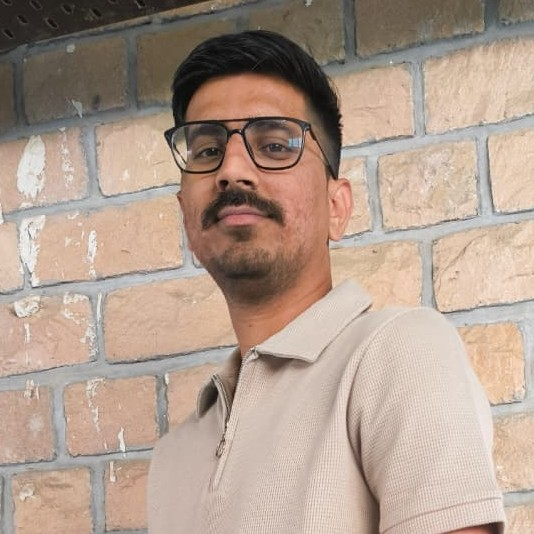
\includegraphics[width=2.5cm]{images/author.jpg}};
  \end{scope}
  \draw[cvNeonCyan, line width=2.0pt] ($(C)+(-5.8, 0.1)$) circle (1.25);
  
  % Author details (glowing white / neon cyan)
  \node[anchor=west, text=cvNeonCyan, font=\cvHH\fontsize{16}{20}\selectfont] 
        at ($(C)+(-4.2, 1.4)$) {कृष्ण कुमार गोदारा};
        
  \node[anchor=north west, text width=10.4cm, align=justify, text=white, font=\cvBH\fontsize{9.5}{13.5}\selectfont] 
        at ($(C)+(-4.3, 1.0)$) {%
    भारतीय प्रौद्योगिकी संस्थान (IIT) जोधपुर में भौतिकी विभाग के अंतर्गत PhD शोधार्थी (JRF)
    हैं। उनका शोध कार्य सक्रिय पदार्थ (Active Matter), गैर-संतुलन प्रणालियों तथा कम्प्यूटेशनल
    भौतिकी पर केंद्रित है।\par\smallskip
    उन्होंने \textbf{CSIR-UGC NET-JRF 2024 (भौतिक विज्ञान)} में अखिल भारतीय रैंक \textbf{46}
    प्राप्त की। उनका उद्देश्य आधुनिक विज्ञान, कृत्रिम बुद्धिमत्ता और कम्प्यूटेशनल तकनीकों को
    विद्यार्थियों तक सरल एवं प्रेरणादायक रूप में पहुँचाना है।
  };


  % ---------------- 3. संपर्क सूत्र (QR Codes) ----------------
  \node[draw=cvNeonCyan, line width=1.2pt, fill=white, inner sep=1.5pt, rounded corners=2pt] 
        (linkedin) at ($(C)+(-4.5, -4.5)$) {
\includegraphics[width=2.1cm]{images/Linkedin.png}};
  \node[draw=cvNeonCyan, line width=1.2pt, fill=white, inner sep=1.5pt, rounded corners=2pt] 
        (instagram) at ($(C)+(0, -4.5)$) {
\includegraphics[width=2.1cm]{images/Instagram.png}};
  \node[draw=cvNeonCyan, line width=1.2pt, fill=white, inner sep=1.5pt, rounded corners=2pt] 
        (github) at ($(C)+(4.5, -4.5)$) {
\includegraphics[width=2.1cm]{images/github.png}};


  % ---------------- 4. उद्धरण एवं चित्र (Bottom Quote Card) ----------------
  % AI Core (Left)
  \fill[cvBgDark, draw=cvNeonCyan, line width=2pt] ($(C)+(-6.8, -9.2)$) circle (1.1);
  \pic[scale=1.3] at ($(C)+(-6.8, -9.2)$) {chip};
  
  % Speech bubble/rounded card for quote (neon purple frame)
  \filldraw[fill=cvBgLight!35!cvBgDark, draw=cvNeonPurple, line width=1.5pt, rounded corners=12pt] 
           ($(C)+(-4.5, -10.8)$) rectangle ($(C)+(7.2, -7.6)$);
           
  % Quote Text (white/neon orange)
  \node[text width=11.0cm, align=center, text=white, font=\cvHH\fontsize{14}{20}\selectfont] 
        at ($(C)+(1.35, -9.2)$) {%
    \color{white} “आज की जिज्ञासा, कल की खोज बनती है;\\
    और {\color{cvNeonOrange}कृत्रिम बुद्धिमत्ता} उस खोज को नई दिशा देती है।”
  };
  
  % Graphics on the right
  \pic[scale=0.8, rotate=30] at ($(C)+(8.4, -9.5)$) {rocket};
  \pic[scale=0.5] at ($(C)+(6.8, -7.5)$) {atom};


  % ---------------- 5. संस्करण एवं बारकोड (Bottom-most details) ----------------
  % Left edition text
  \node[anchor=west, text=cvNeonCyan, font=\cvHH\fontsize{9.5}{12}\selectfont] 
        at ($(C)+(-8.5, -13.2)$) {
    प्रथम संस्करण (First Edition) ~$\cdot$~ 2026\\[2pt]
    \color{white!80} स्वप्रकाशित (Self-published)
  };
  
  % Right barcode (white container with neon border)
  \node[anchor=east] at ($(C)+(8.5, -12.8)$) {
    \fcolorbox{cvNeonCyan}{white}{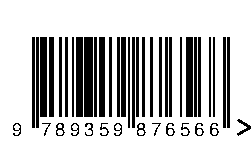
\includegraphics[height=1.5cm]{images/isbn-barcode.pdf}}
  };
  \node[anchor=east, text=white, font=\cvHH\fontsize{8.5}{10}\selectfont] 
        at ($(C)+(8.5, -13.9)$) {ISBN 978-93-5987-656-6};

\end{tikzpicture}
\clearpage


\end{document}
